\documentclass{beamer}
\usepackage{tikz}
\usepackage{gillius}
\usepackage{abraces}
\usepackage{etex}
\usepackage{array}
\usepackage{multirow}
\usepackage{qrcode}
\usepackage[backend=biber, style=numeric-comp, sorting=none]{biblatex}

% http://tex.stackexchange.com/questions/12703/how-to-create-fixed-width-table-columns-with-text-raggedright-centered-raggedlef
\newcolumntype{L}[1]{>{\raggedright\let\newline\\\arraybackslash\hspace{0pt}}m{#1}}
\newcolumntype{C}[1]{>{\centering\let\newline\\\arraybackslash\hspace{0pt}}m{#1}}
\newcolumntype{R}[1]{>{\raggedleft\let\newline\\\arraybackslash\hspace{0pt}}m{#1}}

\usetikzlibrary{external}
\usetikzlibrary{shapes}
\usetikzlibrary{arrows}
\usetikzlibrary{positioning}
\usetikzlibrary{decorations.pathreplacing}
\usetikzlibrary{calc}

\usetheme[everytitleformat=regular]{m}
\setbeamertemplate{navigation symbols}{}

\graphicspath{{../figures/}}
\newcommand{\tablepath}{../tables}

\title{Phylogenetic inference of contact network parameters with approximate Bayesian computation}
\author[RMM \& AFYP]{Rosemary M McCloskey$^1$ \and Bioinformatics Training Program \\ Supervisor: Art FY Poon$^{1,2}$}
\institute[UBC \& BCCfE]{$^1$BC Centre for Excellence in HIV/AIDS, Vancouver, Canada \\ $^2$Department of Medicine, University of British Columbia, Vancouver, Canada}
\date{M.Sc. Defence, July 26, 2016}

\newcommand{\dd}[2]{\frac{\text{d}\,#1}{\text{d}\,#2}}

\addbibresource{papers.bib}

\begin{document}
\setbeamercolor{background canvas}{bg=white}
\renewcommand{\footnotesize}{\tiny}
\definecolor{red}{RGB}{228,26,28}
\definecolor{blue}{RGB}{55,126,184}
\definecolor{green}{RGB}{77,175,74}
\definecolor{purple}{RGB}{152,78,163}

\maketitle

\begin{frame}{Modeling in epidemiology}
  \centerline{\includegraphics[width=0.9\textwidth]{compartments}}
\end{frame}

\begin{frame}{Contact heterogeneity can affect epidemic expansion}
  \centerline{\includegraphics[width=0.9\textwidth]{sir-trajectories}}
\end{frame}

\begin{frame}{Contact networks capture contact heterogeneity}
  \begin{center}
  \begin{tikzpicture}
    \node (c) {\includegraphics[width=4cm]{contactnet-empty}};

    \uncover<2->{
    \node (a) [right=of c.north east, anchor=west] {nodes = individuals};
    \draw [->, thick, >=stealth] (c.north east) ++(-1.5cm, -0.5cm) -- (a.west);
    }

    \uncover<3->{
    \node (b) [below=0.5 of a] {edges = contacts};
    \draw [->, thick, >=stealth] (c.north east) ++(-0.75cm, -1.25cm) -- (b.west);
    }
  \end{tikzpicture}
  \end{center}
\end{frame}

\begin{frame}{Network models formally describe network structure}
  \begin{columns}
    \column{0.55\textwidth}
    \begin{minipage}[c][.6\textheight][c]{\linewidth}
      \begin{enumerate}
        \setlength{\itemsep}{12pt}
        \item Start with \only<1-4>{10}\only<5->{\alert{$n$}} women and 
          \only<1-4>{10}\only<5->{\alert{$n$}} men.
        \uncover<2->{
        \item Randomly form \only<2-4>{20}\only<5->{\alert{$p \times n$}} male-female partnerships.
        }
        \uncover<3->{
        \item Randomly rewire each edge with \only<3-4>{10}\only<5->{\\\alert{$q$ }}\% probability.
        }
      \end{enumerate}
    \end{minipage}
    \column{0.5\textwidth}
    \begin{minipage}[c][.6\textheight][c]{\linewidth}
      \only<1>{\includegraphics[width=5cm, page=1]{homophily}}
      \only<2>{\includegraphics[width=5cm, page=2]{homophily}}
      \only<3>{\includegraphics[width=5cm, page=3]{homophily}}
      \only<4->{\includegraphics[width=5cm, page=4]{homophily}}
    \end{minipage}
  \end{columns}

  \vspace{0.5cm}
  \begin{columns}
    \column{0.55\textwidth}
    \uncover<6->{\centerline{\large{network model}}}
    \column{0.55\textwidth}
    \uncover<6->{\centerline{\large{contact network}}}
  \end{columns}
\end{frame}

\begin{frame}{Barab\'asi-Albert model incorporates preferential attachment}
  \begin{columns}
  \column{0.5\textwidth}
  \begin{tikzpicture}[
      scale=2,
      every edge/.style={thick}
    ]
    \node (n1) at (1, 0) [circle, fill=black] { };
    \node (n2) at (0.86, 0.5) [circle, fill=black] { };
    \node (n3) at (0.5, 0.86) [circle, fill=black] { };
    \draw (n1) -- (n2) -- (n3) -- (n1);

    \uncover<2->{
      \node (n4) at (0, 1) [circle, fill=black] { };
    }
    \only<2-3>{
      \node [right=0 of n4.north east, anchor=south west] {$m = 2$};
    }
    \only<2-4>{
      \draw (n4) -- ++ (0.2, -0.2);
      \draw (n4) -- ++ (-0.2, -0.2);
    }

    \node [right=0 of n1] {%
      \only<3-4>{$\Pr \propto 2^\alpha$}%
      \only<6-7>{$\Pr \propto 3^\alpha$}%
    };
    \node [right=0 of n2] {%
      \only<3-4>{$\Pr \propto 2^\alpha$}%
      \only<6-7>{$\Pr \propto 3^\alpha$}%
    };
    \node [right=0 of n3] {%
      \only<3-4>{$\Pr \propto 2^\alpha$}%
      \only<6-7>{$\Pr \propto 2^\alpha$}%
    };

    \only<4>{
      \draw (n4) -- ++ (0.2, -0.2) -- (n2);
      \draw (n4) -- ++ (-0.2, -0.2) -- (n1);
    }

    \uncover<5->{
      \draw (n4) -- (n2);
      \draw (n4) -- (n1);
    }

    \uncover<6->{
      \node (n5) at (-0.5, 0.86) [circle, fill=black] { };
    }

    \only<6-7> {
      \draw (n5) -- ++ (0.2, -0.2);
      \draw (n5) -- ++ (-0.2, -0.2);
    }
    
    \uncover<6-7>{ \node [right=0 of n4.north east, anchor=south west] { $\Pr \propto 2^\alpha$ }; }

    \only<7>{
      \draw (n5) -- ++ (0.2, -0.2) -- (n3);
      \draw (n5) -- ++ (-0.2, -0.2) -- (n2);
    }

    \uncover<8->{
      \draw (n5) -- (n3);
      \draw (n5) -- (n2);
    }
    
    \uncover<9->{
      \node (n6) at (-0.86, 0.5) [circle, fill=black] { };
      \draw (n6) -- (n2);
      \draw (n6) -- (n1);
    }

    \uncover<10->{
      \node (n7) at (-1, 0) [circle, fill=black] { };
      \draw (n7) -- (n3);
      \draw (n7) -- (n4);
    }

    \uncover<11->{
      \node (n8) at (-0.86, -0.5) [circle, fill=black] { };
      \node (n9) at (-0.5, -0.86) [circle, fill=black] { };
      \node (n10) at (0, -1) [circle, fill=black] { };
      \node (n11) at (0.5, -0.86) [circle, fill=black] { };
      \node (n12) at (0.86, -0.5) [circle, fill=black] { };

      \draw (n8) -- (n2);
      \draw (n8) -- (n4);
      \draw (n9) -- (n2);
      \draw (n9) -- (n1);
      \draw (n10) -- (n2);
      \draw (n10) -- (n8);
      \draw (n11) -- (n3);
      \draw (n11) -- (n9);
      \draw (n12) -- (n2);
      \draw (n12) -- (n8);
    }

    \uncover<12->{
      \node (n1) at (1, 0) [circle, fill=red] { };
      \node (n2) at (0.86, 0.5) [circle, fill=red] { };
      \node (n5) at (-0.86, 0.5) [circle, fill=red] { };
      \node (n7) at (-0.86, -0.5) [circle, fill=red] { };
      \node (n8) at (-0.5, -0.86) [circle, fill=red] { };

      \draw [ultra thick, red] (n2) -- (n7);
      \draw [ultra thick, red] (n2) -- (n1);
      \draw [ultra thick, red] (n8) -- (n1);
      \draw [ultra thick, red] (n5) -- (n2);
    }

    \only<11>{\node [below=of n10] {$N = 12$};}
    \uncover<12->{\node [below=of n10] {$I = 5$};}
  \end{tikzpicture}

  \column{0.4\textwidth}
  \uncover<2->{
    $m$ = number of new edges per vertex \\
    \hfill\\
  }

  \uncover<3->{
    $\alpha$ = preferential attachment power \\
    \hfill\\
  }

  \uncover<11->{
    $N$ = number of nodes \\
    \hfill\\
  }

  \uncover<12->{
    $I$ = number of infected nodes (prevalence) 
  }
  \end{columns}
\end{frame}

\begin{frame}{Why fit network models?}
  \begin{columns}
    \column{0.33\textwidth}
    \includegraphics[width=0.85\textwidth]{sir-trajectories-vertical}

    \column{0.33\textwidth}
    \uncover<2->{
    \includegraphics[width=0.75\textwidth]{nettypes}
    }

    \column{0.33\textwidth}
    \uncover<3->{
    \begin{tikzpicture}
      \node (pic) { \includegraphics[width=0.75\textwidth]{vaccinate} };
      \node at (pic.east) { 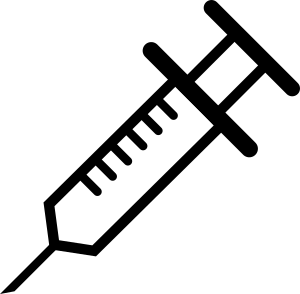
\includegraphics[width=1cm]{stock/syringe} };
    \end{tikzpicture}
    }
  \end{columns}

  \vspace{-0.5cm}

  \begin{columns}
    \column{0.33\textwidth}
    \uncover<1->{
    \centerline{\large predict}
    }

    \column{0.33\textwidth}
    \uncover<2->{
    \centerline{\large characterize}
    }

    \column{0.33\textwidth}
    \uncover<3->{
    \centerline{\large simulate}
    }
  \end{columns}
\end{frame}

\begin{frame}{Phylogenetic methods may help fit network models}
  \begin{itemize}
    \item network models are difficult to fit with conventional epidemiological
      methods (surveys etc.)
    \item sequence data may be easier to collect and free from some biases
      (misreporting etc.)
    \item instead of asking the people, ask the virus! (some cartoon)
  \end{itemize}
\end{frame}

\begin{frame}{Contact networks shape transmission trees}
  \begin{center}
    \begin{tikzpicture}
      [every node/.style = {inner sep=0pt},
       every path/.style = {->, >=stealth, very thick},
       label/.style = {anchor=south, color=white, inner sep=4pt},
       time/.style = {anchor=north west, inner sep=2pt}]
      \def\pht{1cm}
      \node (a) {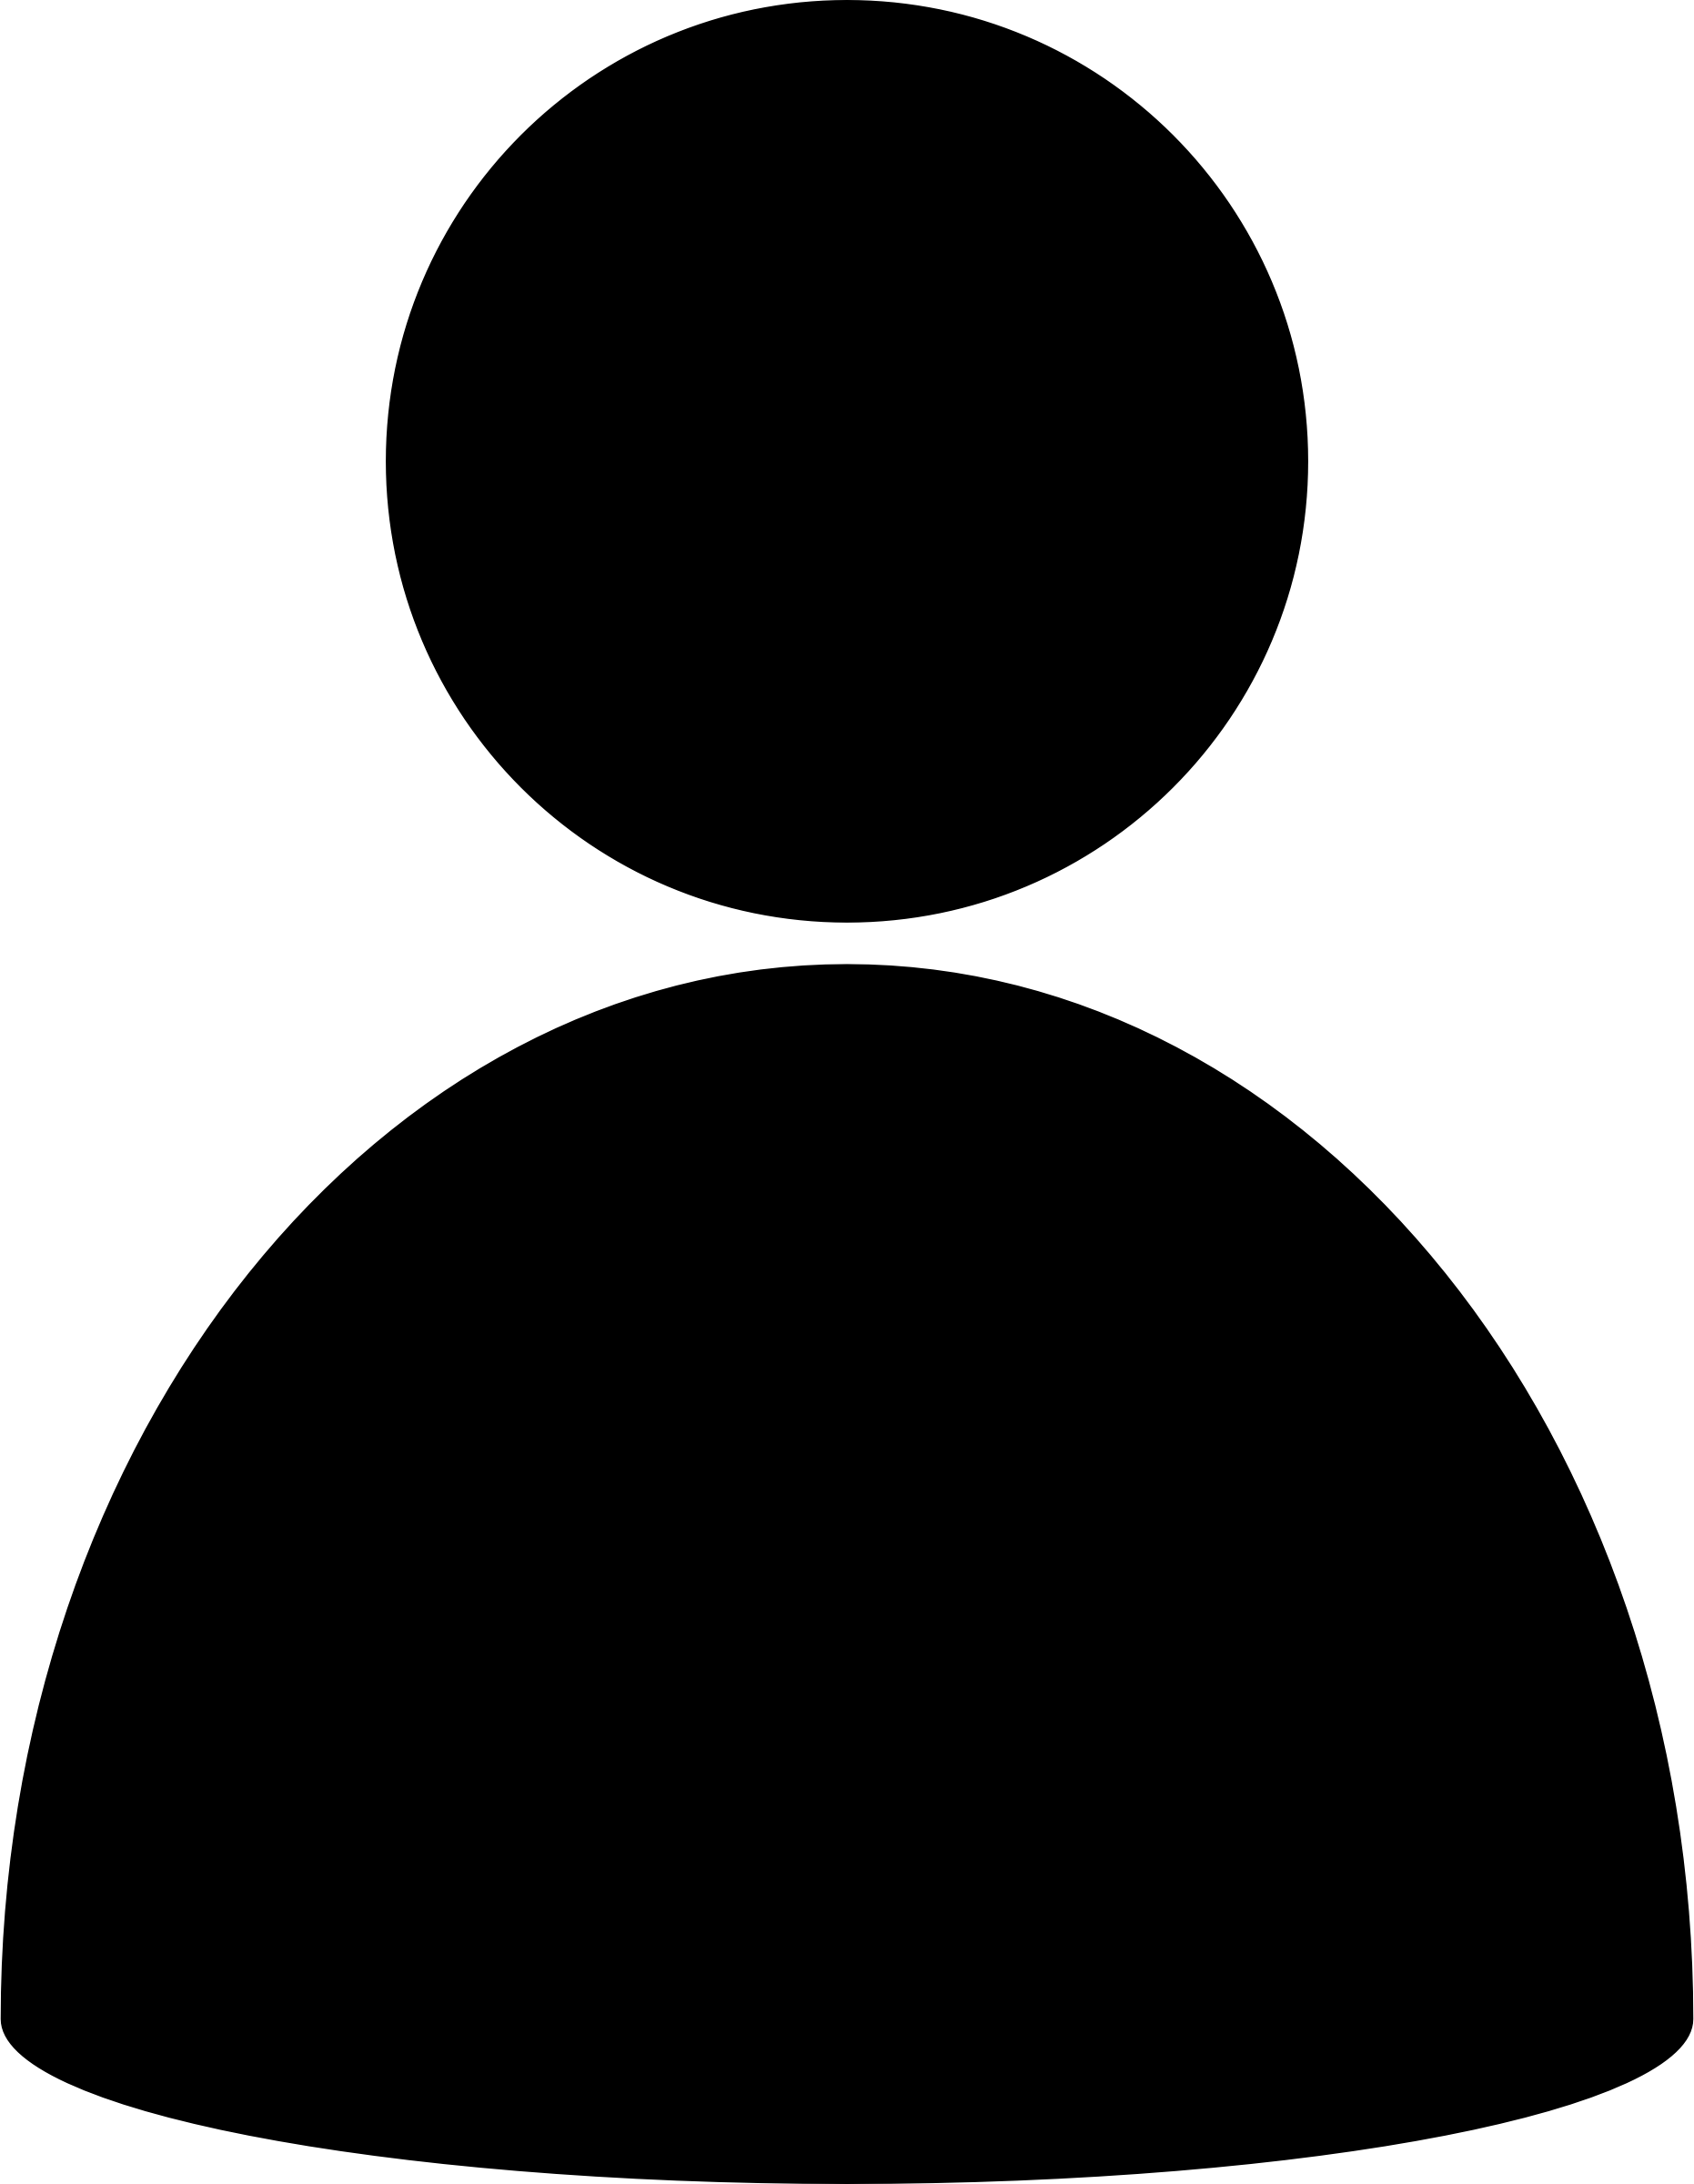
\includegraphics[height=\pht]{stock/person}};
      \node at (a.south) [label] {\Large a};
      \node [below left=0.75 of a] (b) {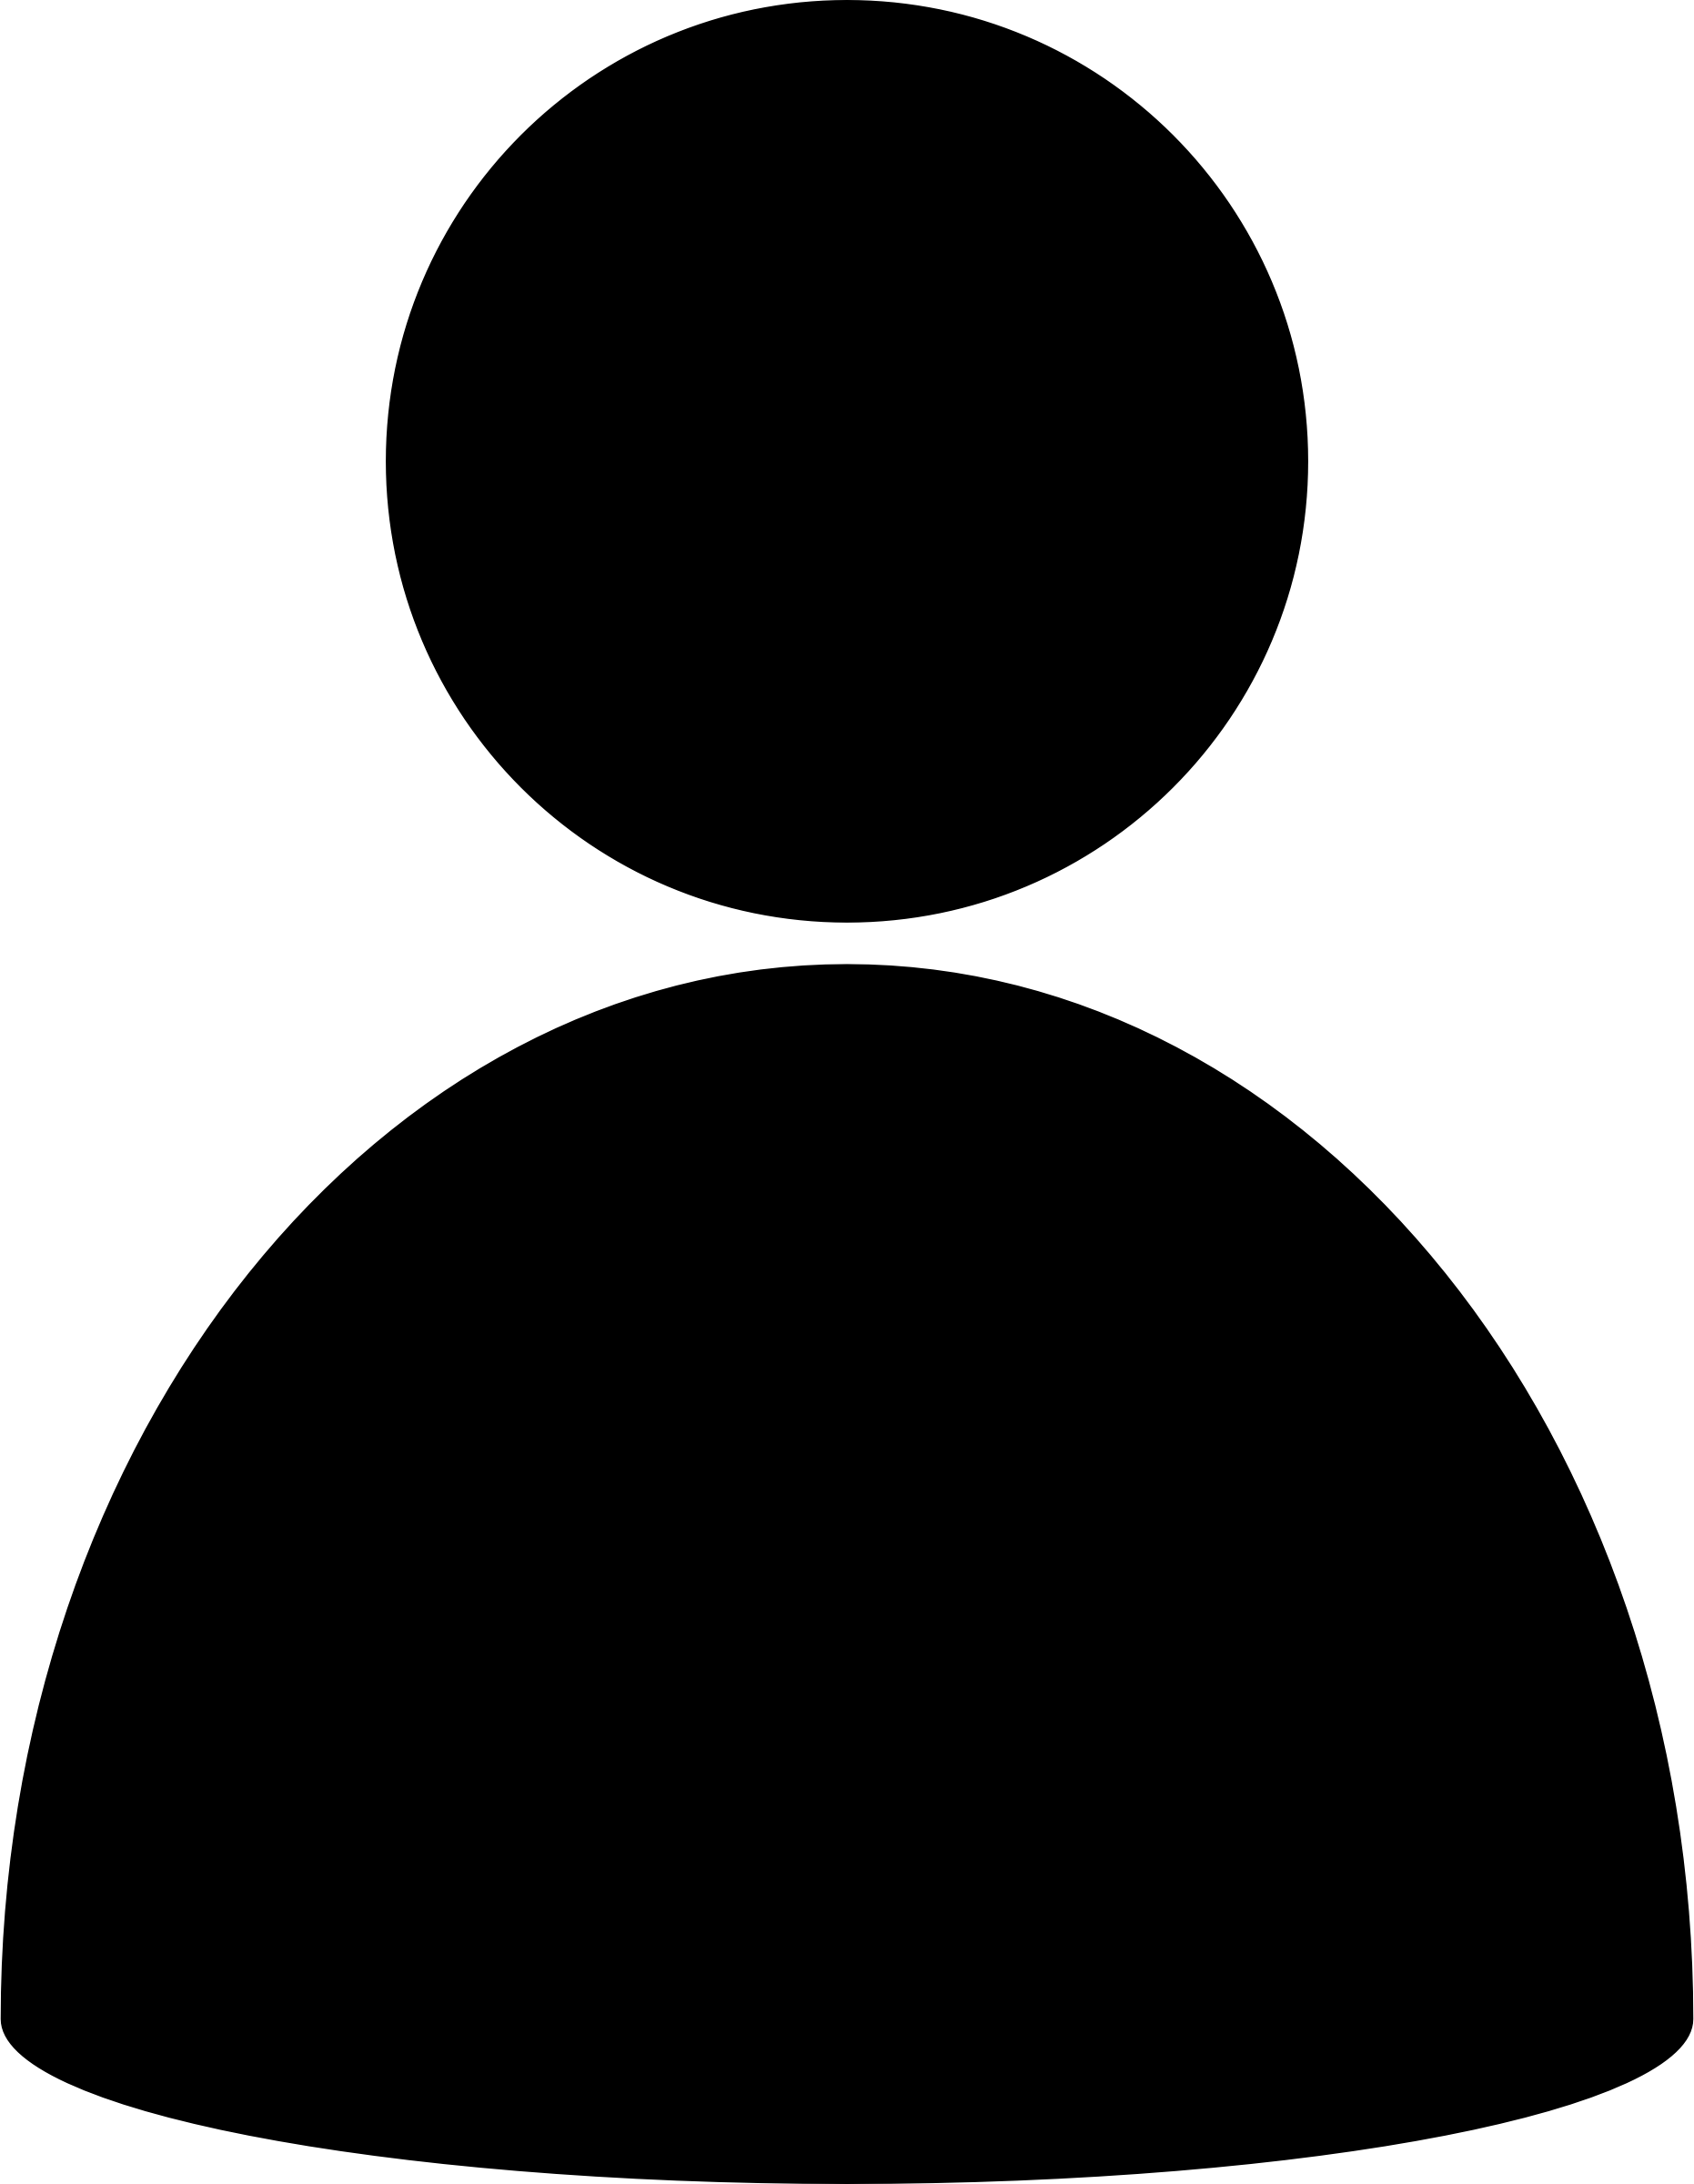
\includegraphics[height=\pht]{stock/person}};
      \node at (b.south) [label] {\Large b};
      \node [below=0.75 of b] (e) {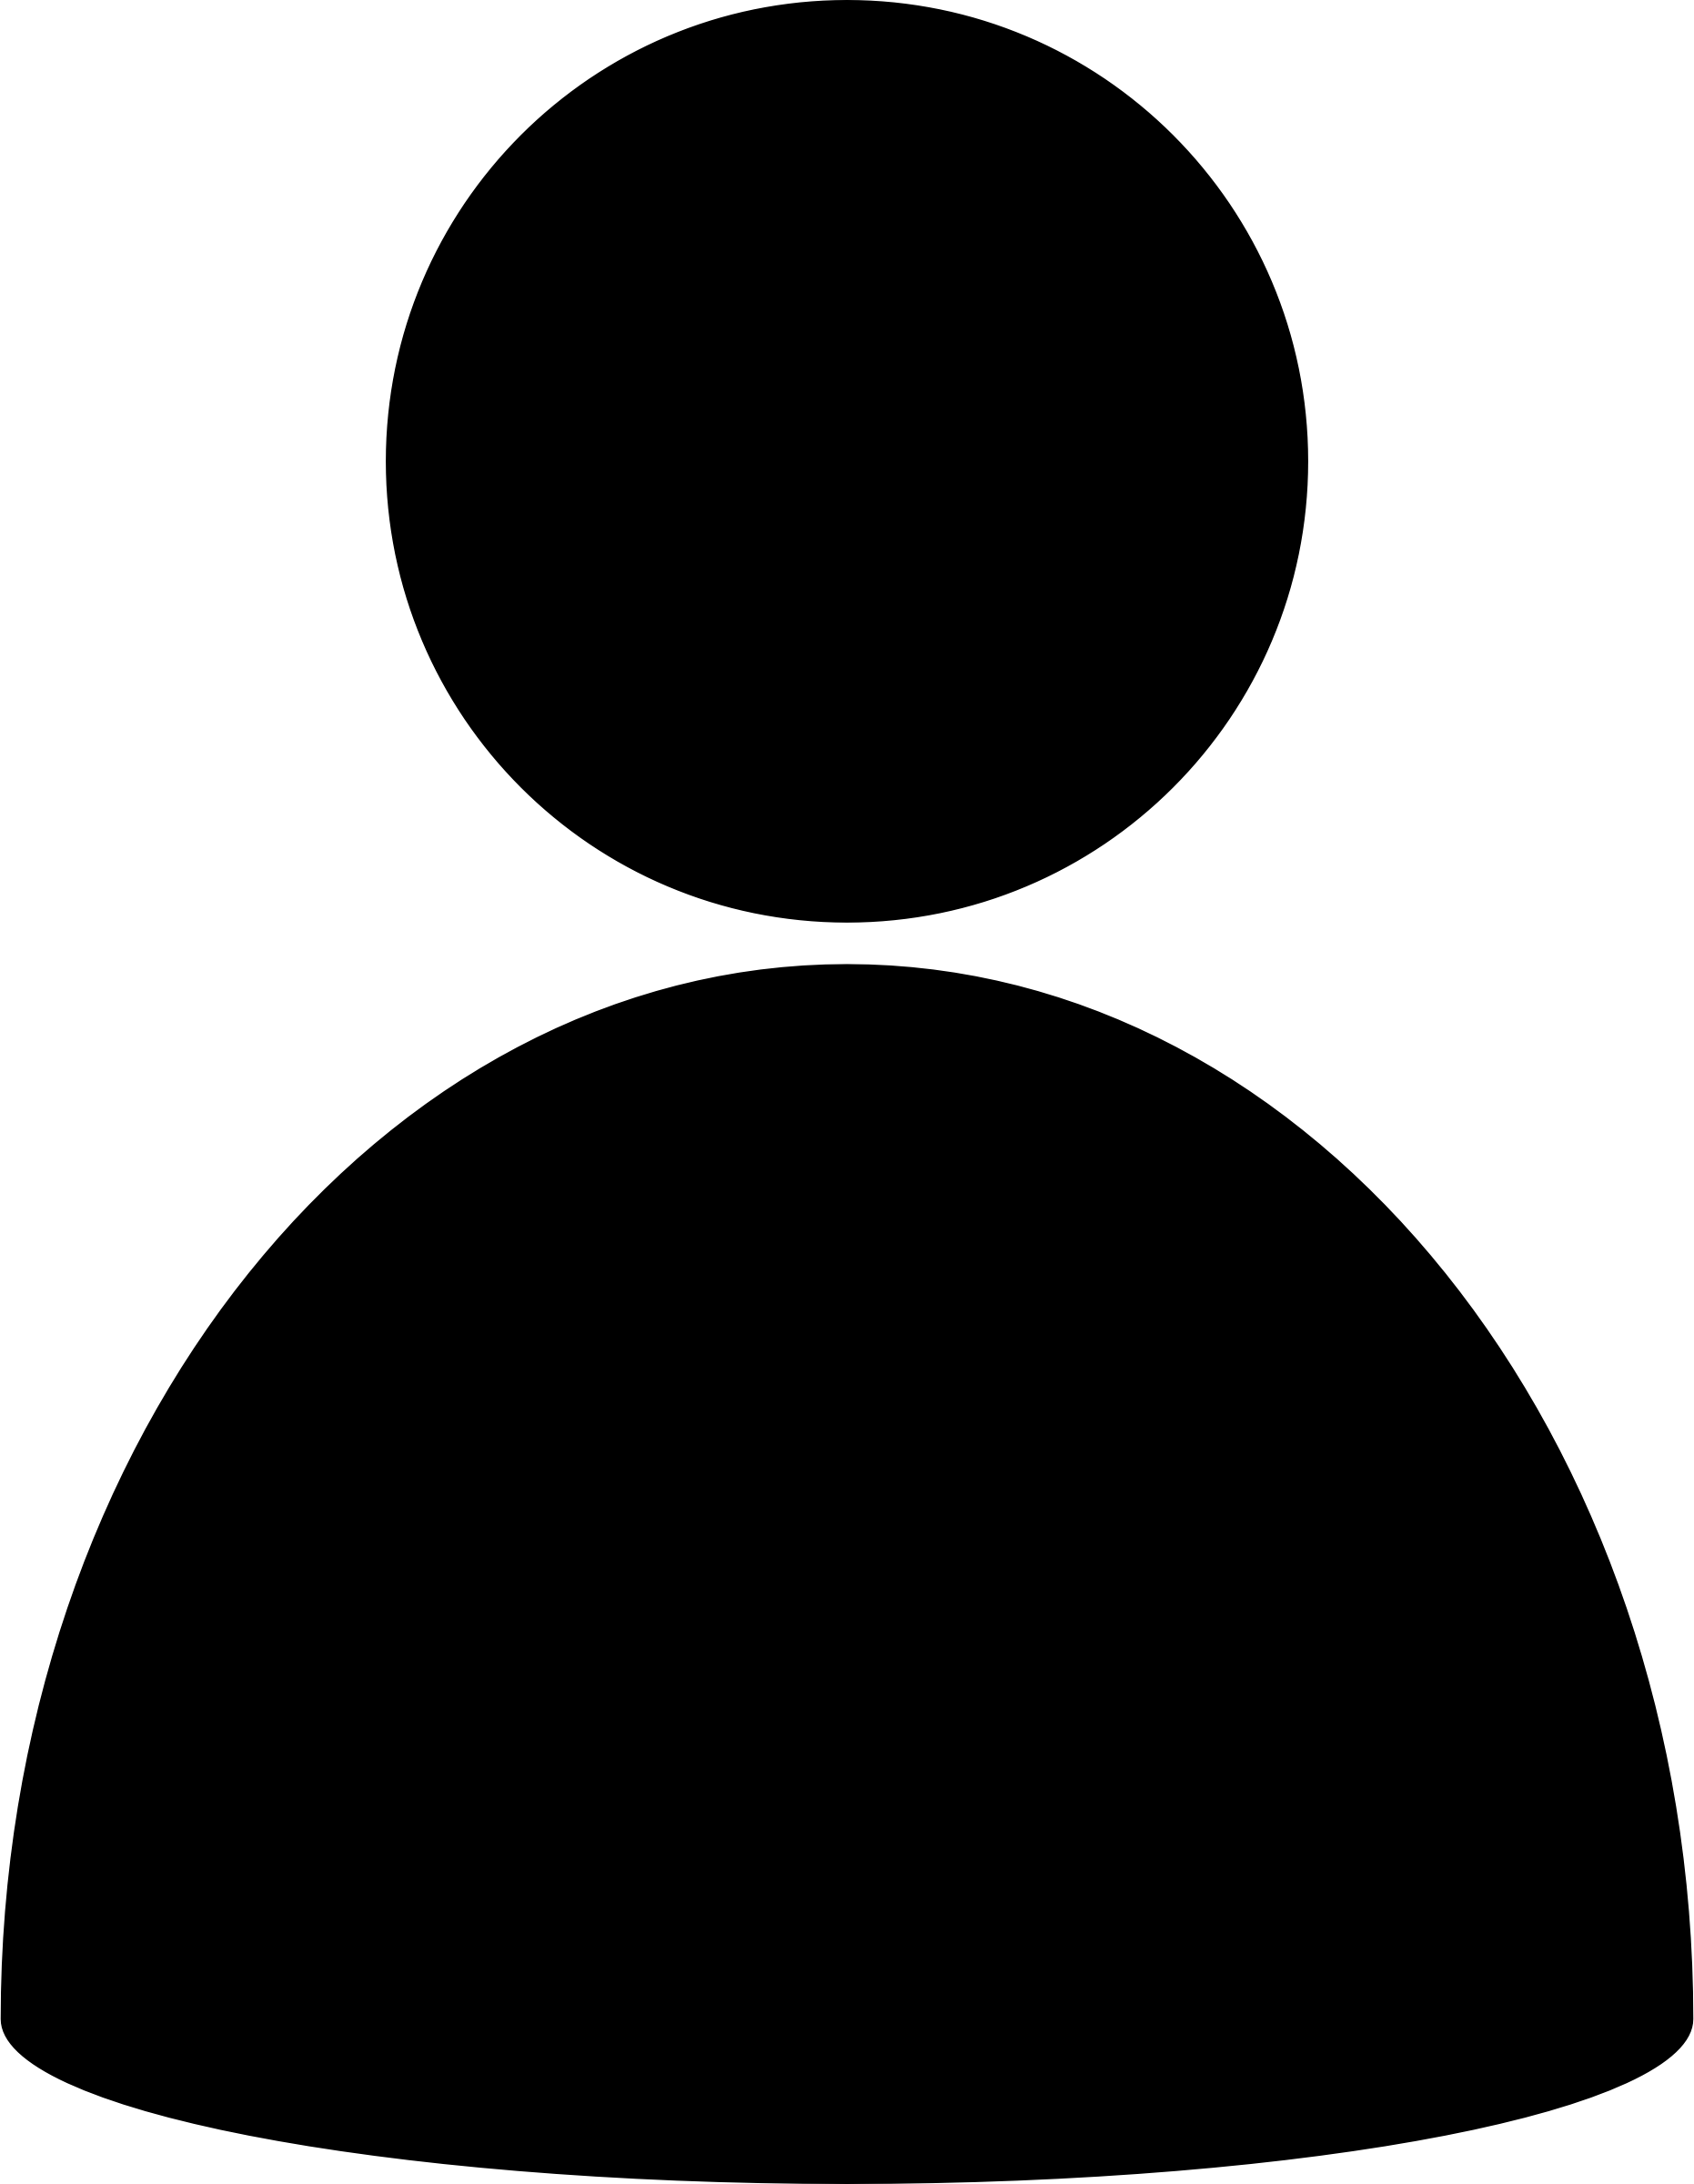
\includegraphics[height=\pht]{stock/person}};
      \node at (e.south) [label] {\Large e};
      \node [below right=0.75 of a] (c) {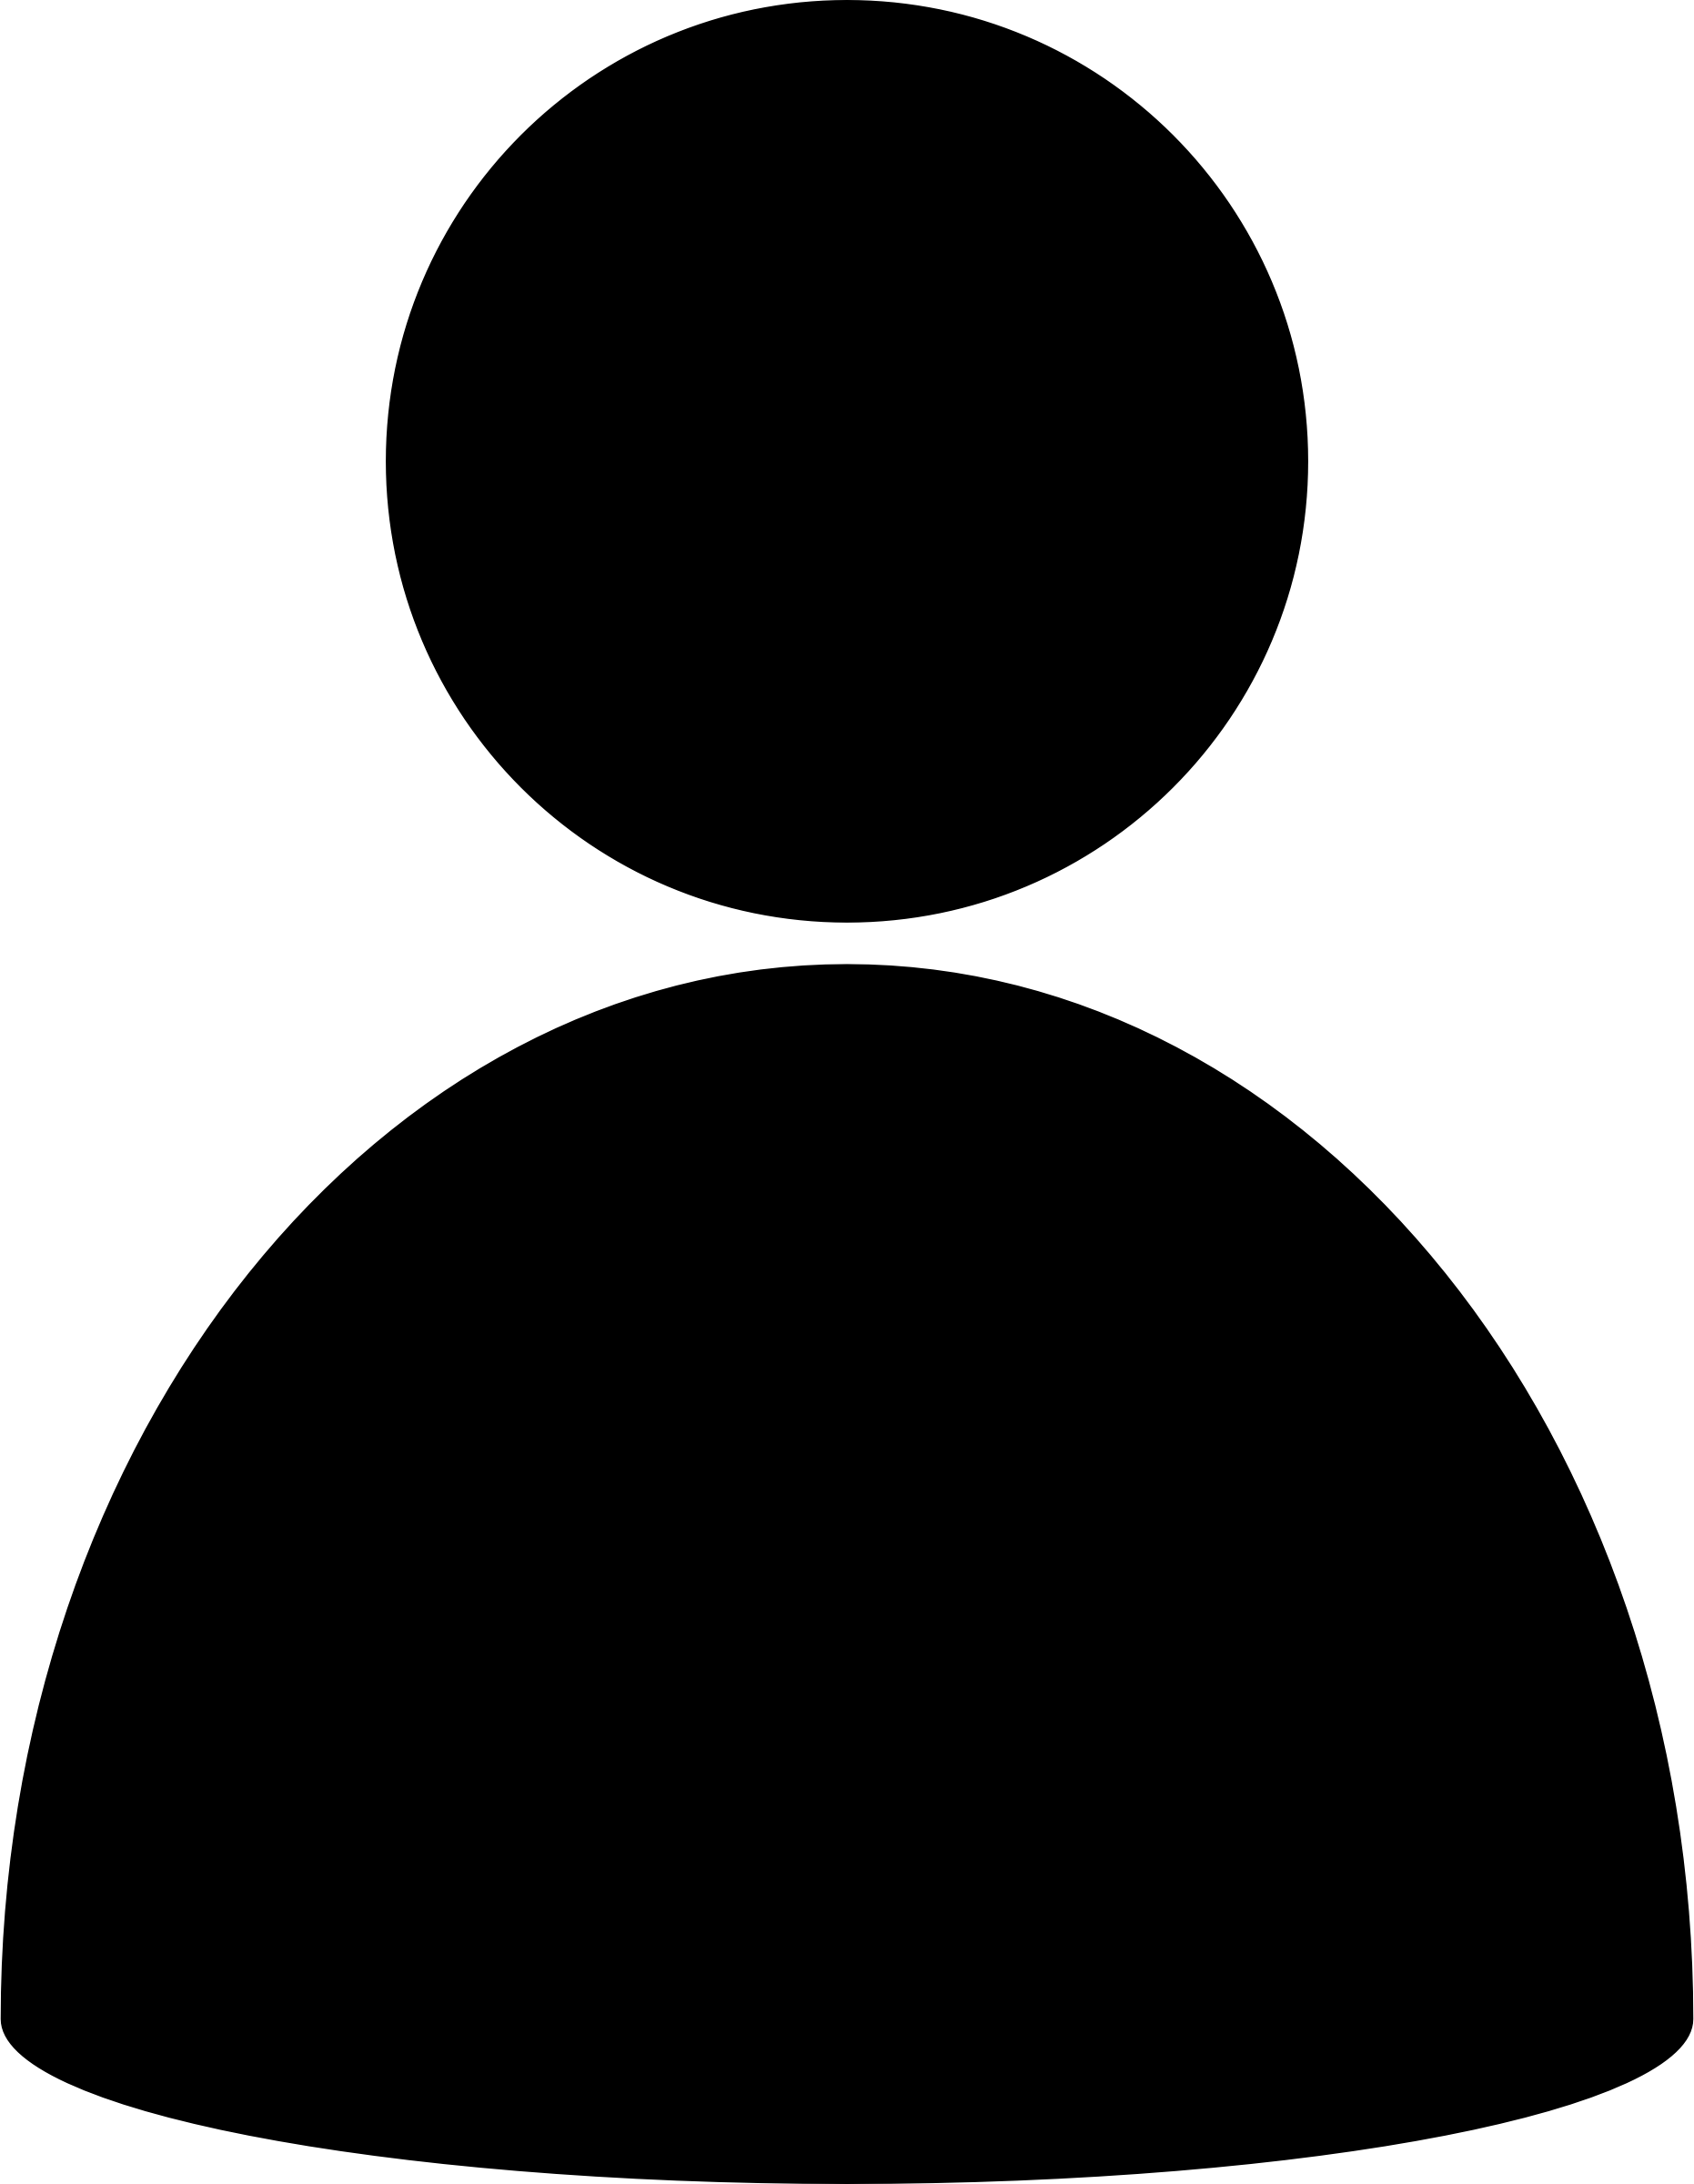
\includegraphics[height=\pht]{stock/person}};
      \node at (c.south) [label] {\Large c};
      \node [below=0.75 of c] (d) {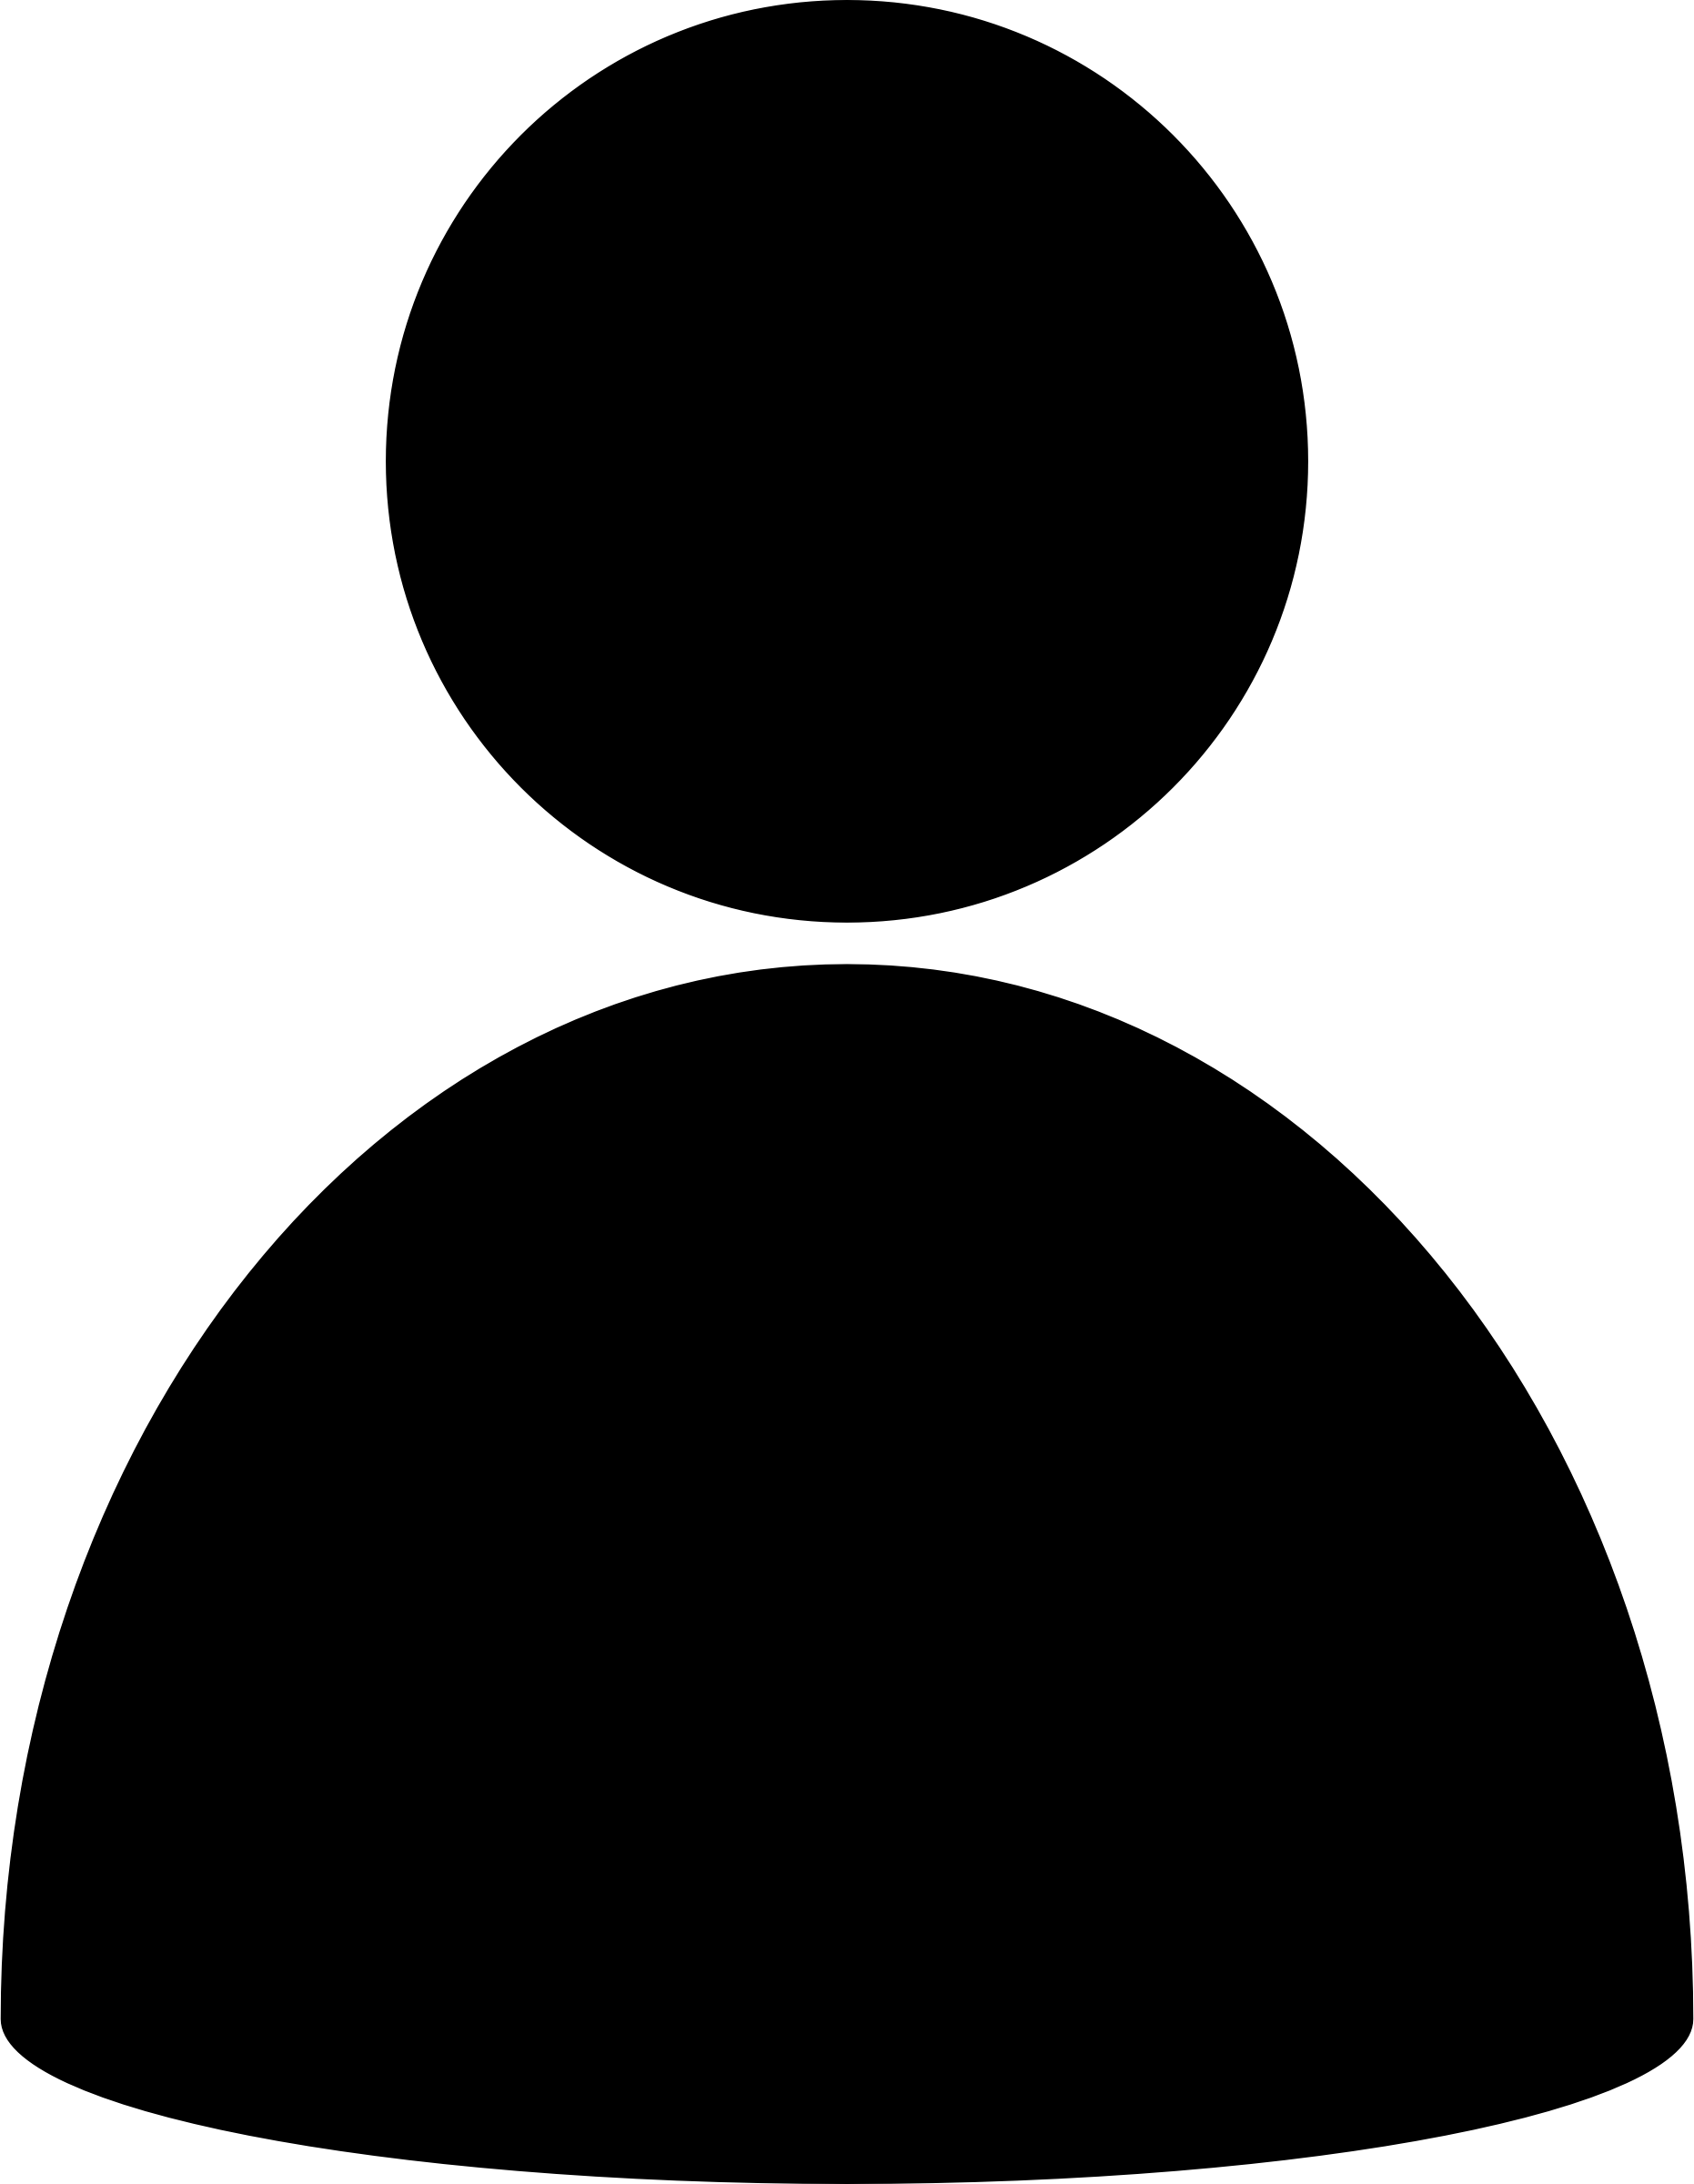
\includegraphics[height=\pht]{stock/person}};
      \node at (d.south) [label] {\Large d};
    
      \fill [shade, opacity=0.2] (a.east) -- (c.north) -- (c.north west) -- (a.south east) -- cycle;
      \uncover<3->{
      \draw [blue] ($(a.east) + (0, -12pt)$) -- ($(c.north) + (-8pt, 0)$);
      }
      \fill [shade, opacity=0.2] (a.west) -- (b.north) -- (b.north east) -- (a.south west) -- cycle;
      \uncover<2->{
      \draw [red] ($(a.west) + (0, -12pt)$) -- ($(b.north) + (8pt, 0)$);
      }
      \fill [shade, opacity=0.2] (a.south) -- (a.south west) -- (e.north) -- (e.north east) -- cycle;
      \fill [shade, opacity=0.2] (b.south west) -- (b.south) -- (e.north) -- (e.north west) -- cycle;
      \fill [shade, opacity=0.2] ($(c.south) + (-8pt, 0)$) -- ++(16pt, 0) -- ($(d.north) + (8pt, 0)$) -- ++(-16pt, 0) -- cycle;
      \fill [shade, opacity=0.2] (b.east) -- (b.south east) -- (d.west) -- (d.north west) -- cycle;
      \uncover<4->{
      \draw [green!80!black] (c) -- (d);
      }

      \node (abcd) [right=6cm of a.north] {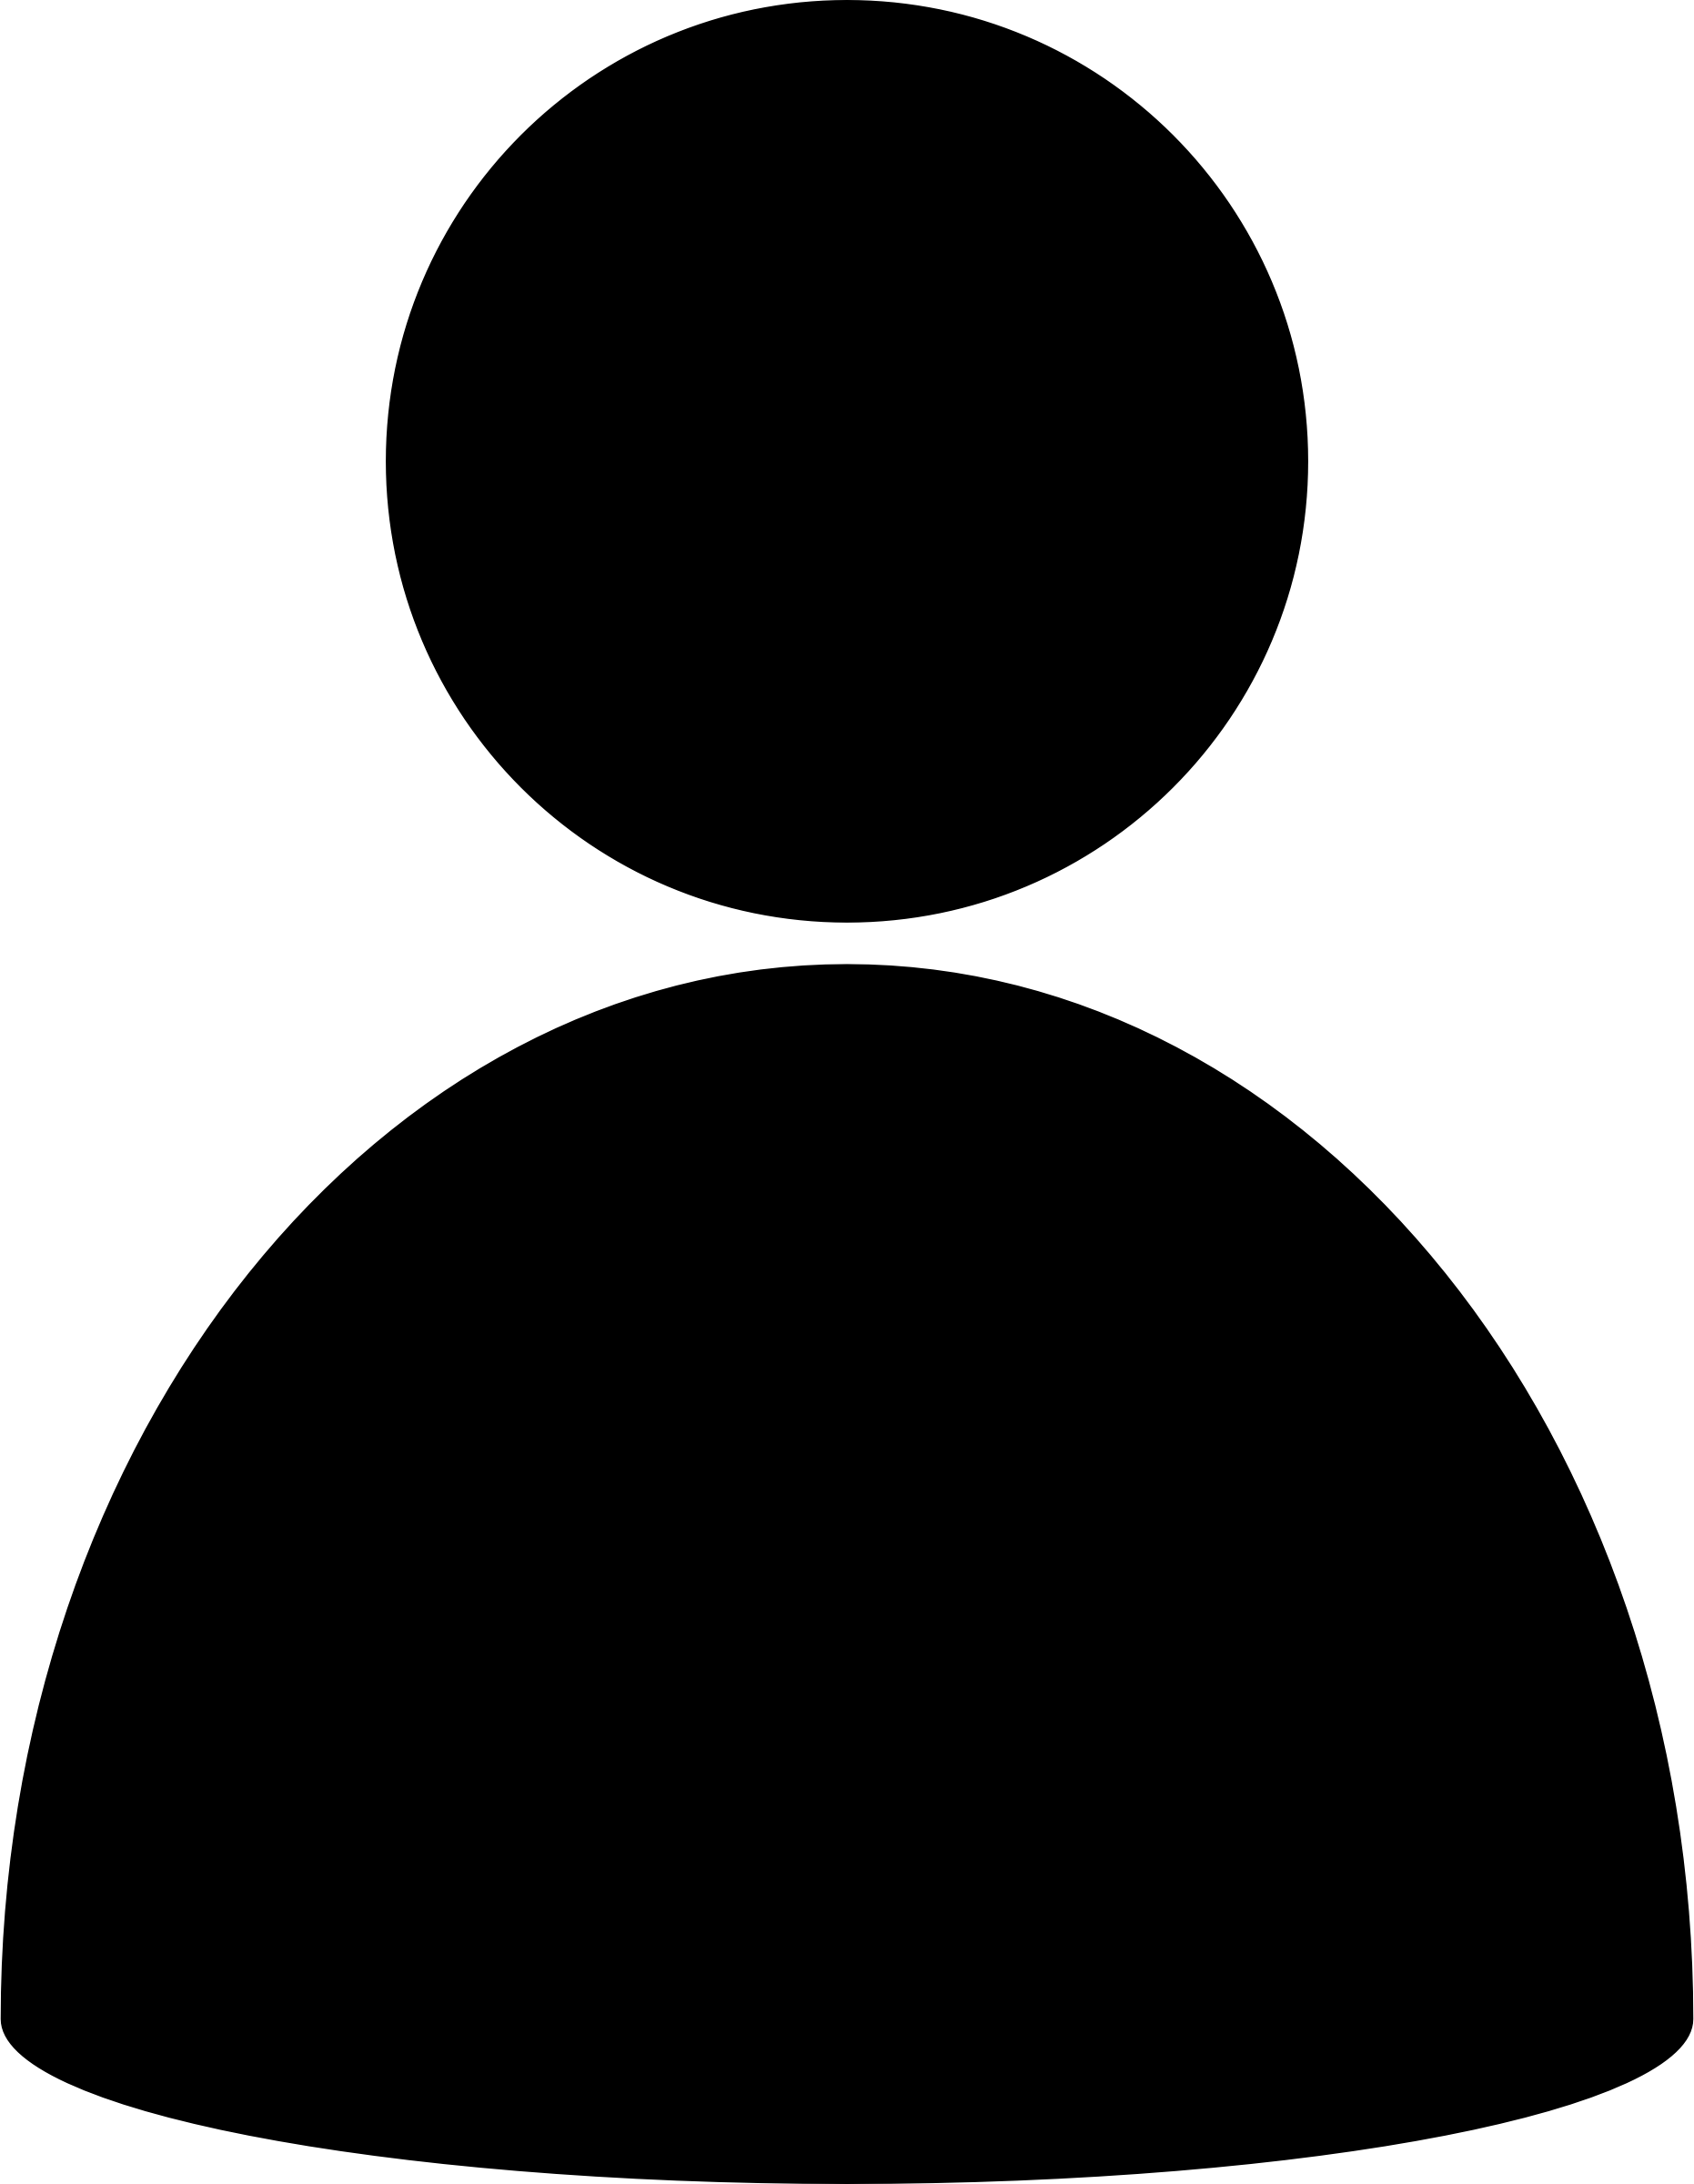
\includegraphics[height=\pht]{stock/person}};
      \node at (abcd.south) [label] {\Large a};
      \uncover<2->{
      \node (b) [below right=1 and 0.75 of abcd] {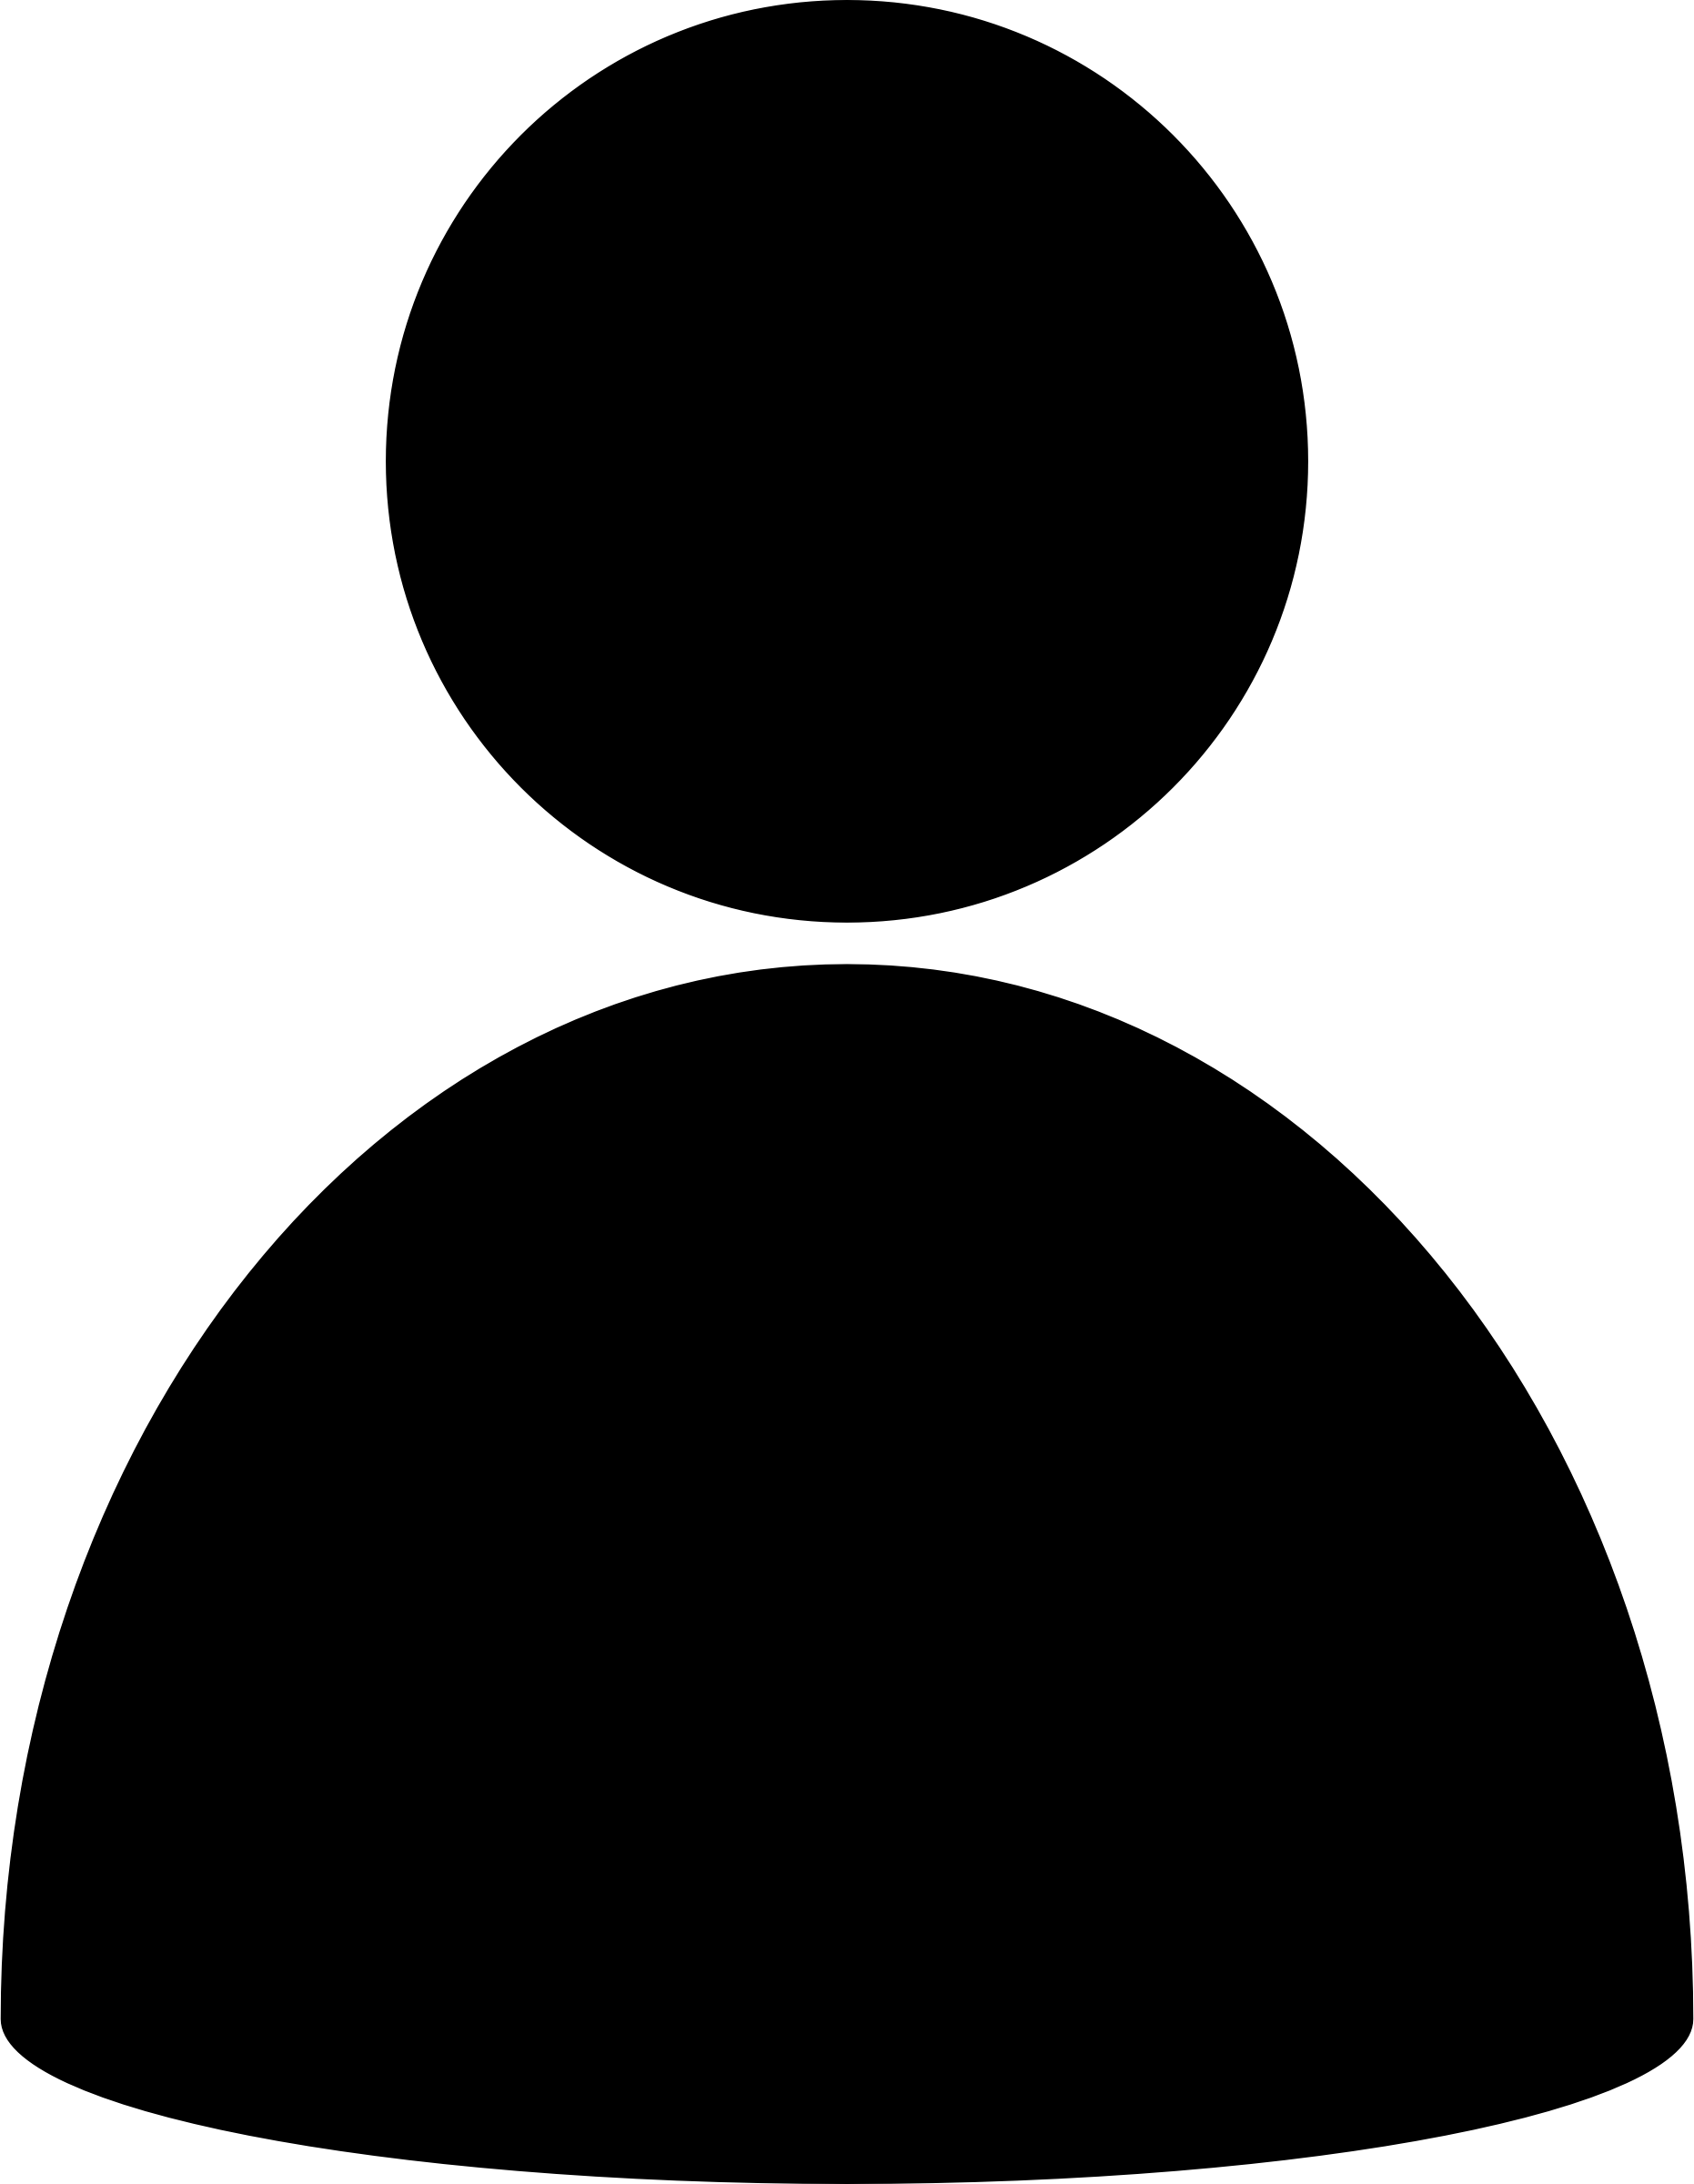
\includegraphics[height=\pht]{stock/person}};
      \node at (b.south) [label] {\Large b};
      \node (acd) [below left=1 and 0.5 of abcd] {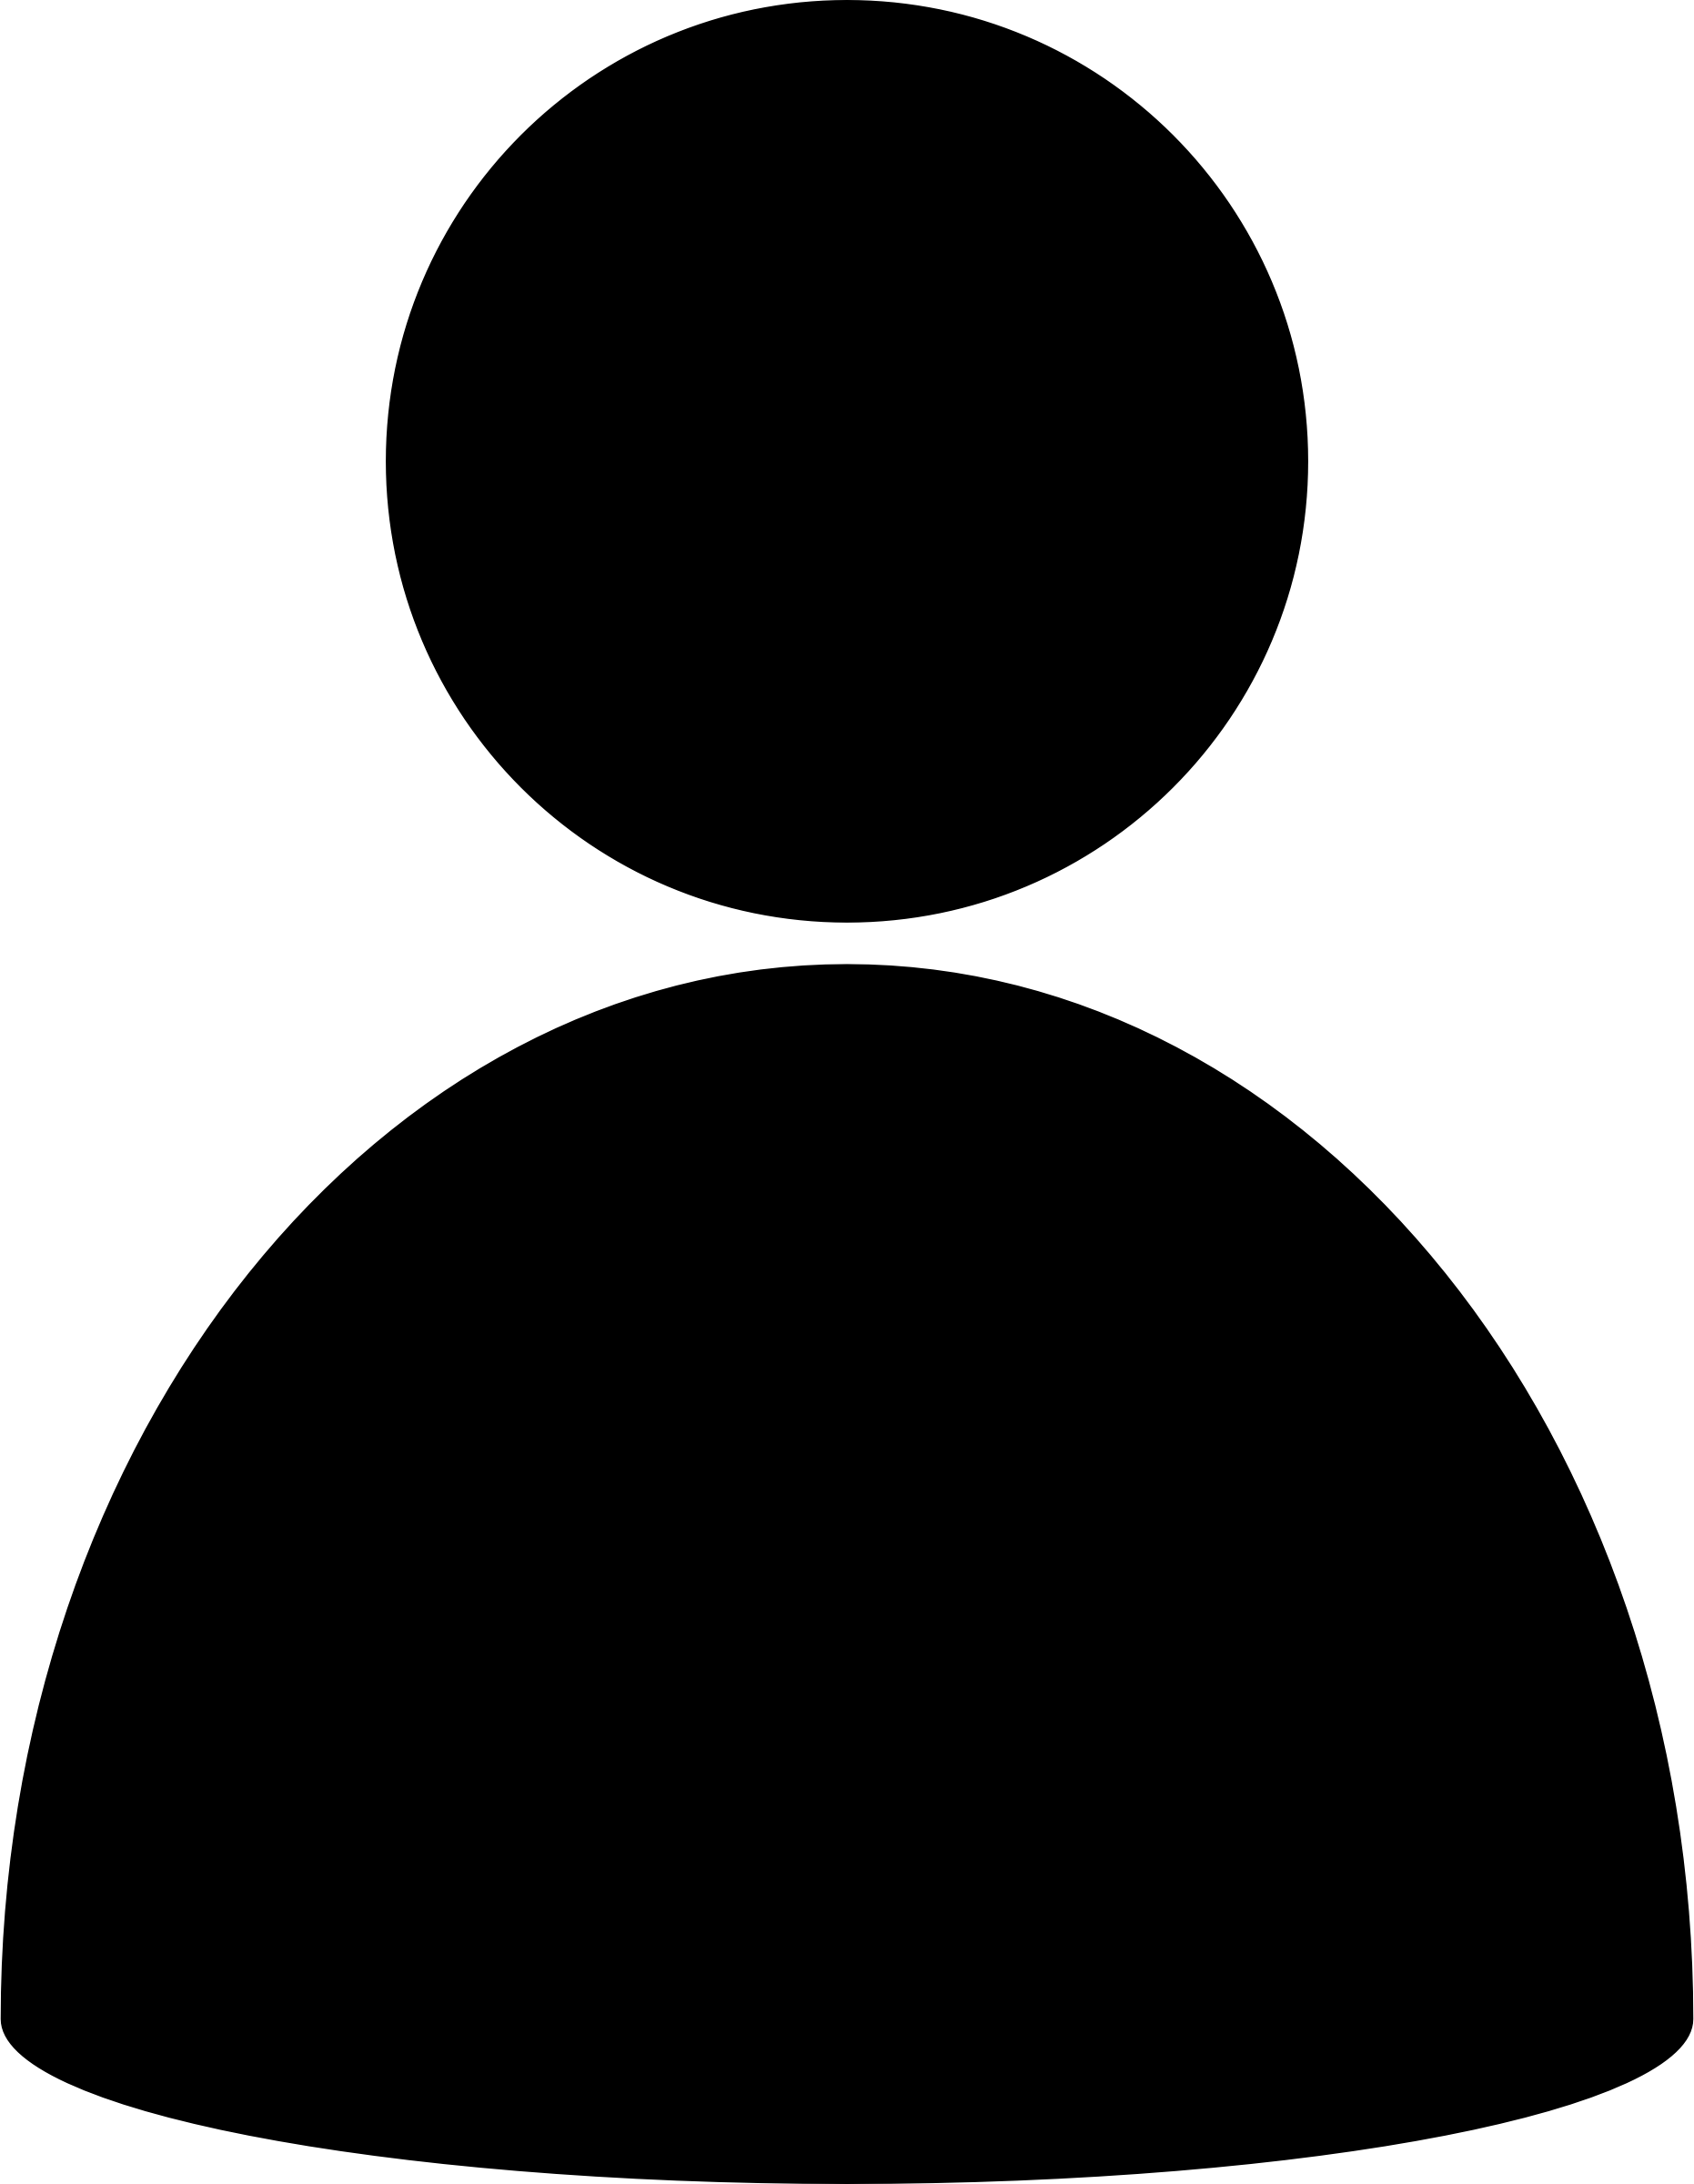
\includegraphics[height=\pht]{stock/person}};
      \node at (acd.south) [label] {\Large a};
      }
      \uncover<3->{
      \node (cd) [below right=0.5 and 0.5 of acd] {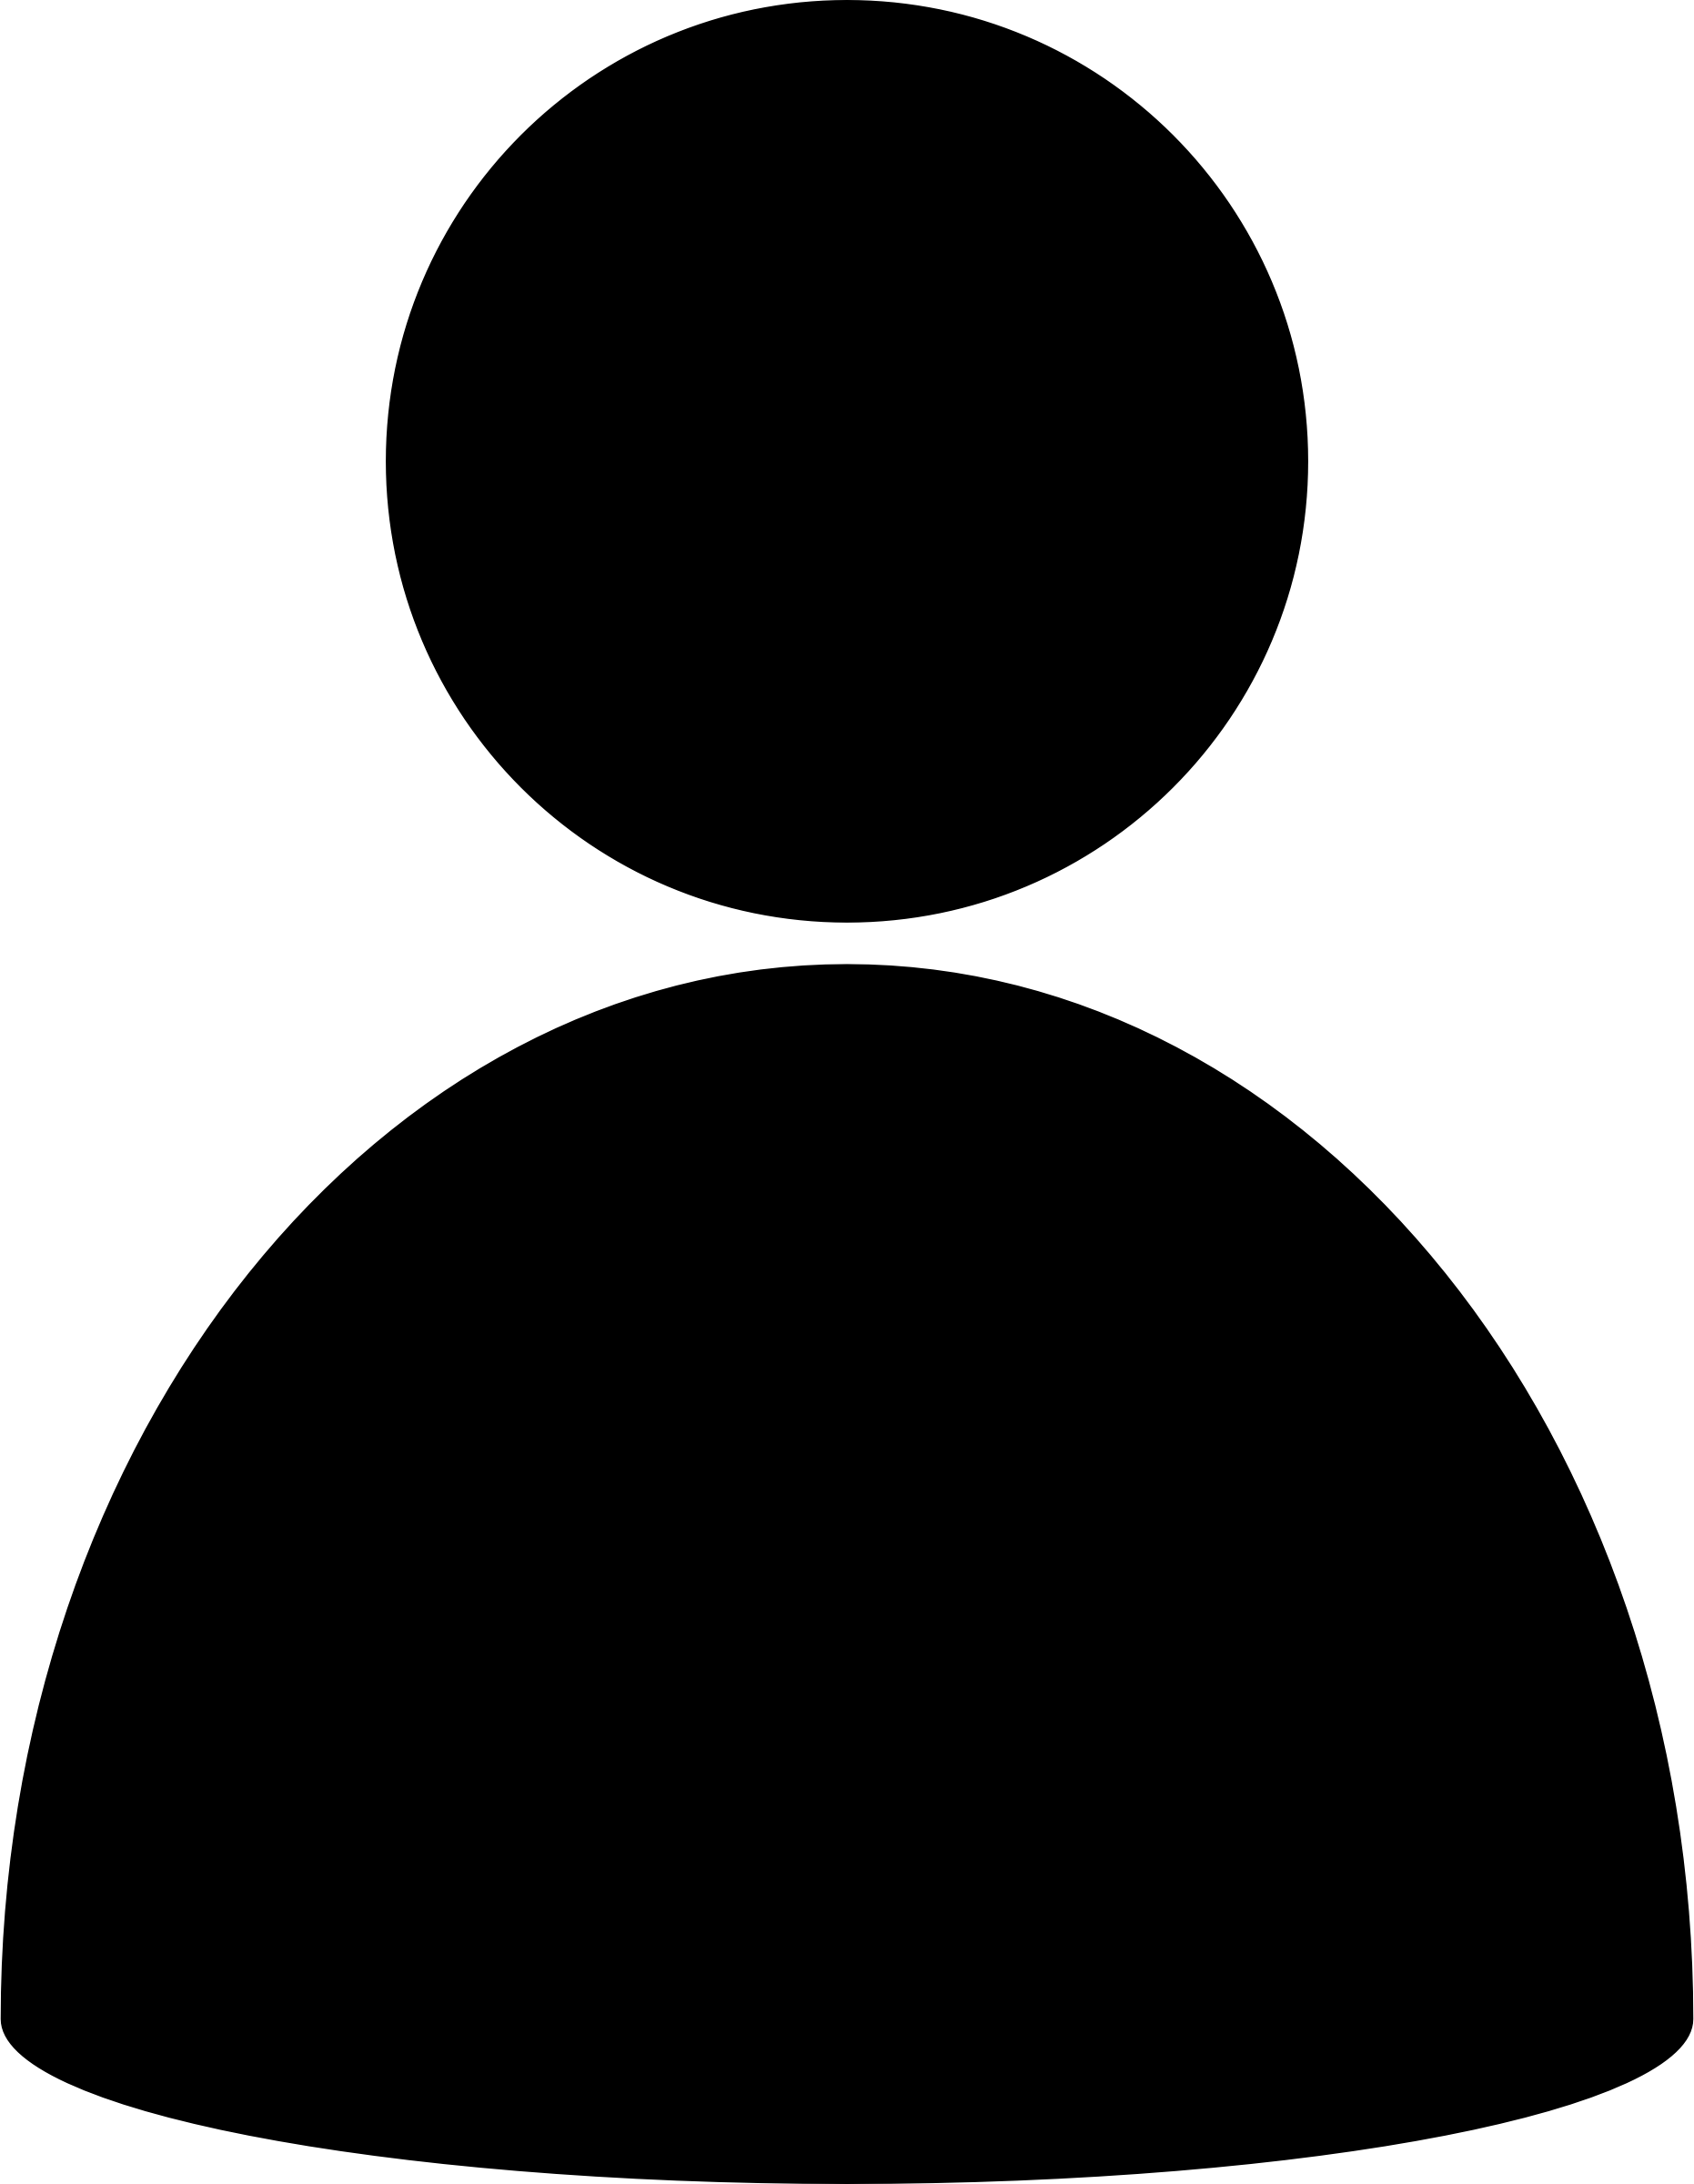
\includegraphics[height=\pht]{stock/person}};
      \node at (cd.south) [label] {\Large c};

      \node (a) [below left=0.25 and 0.25 of acd] {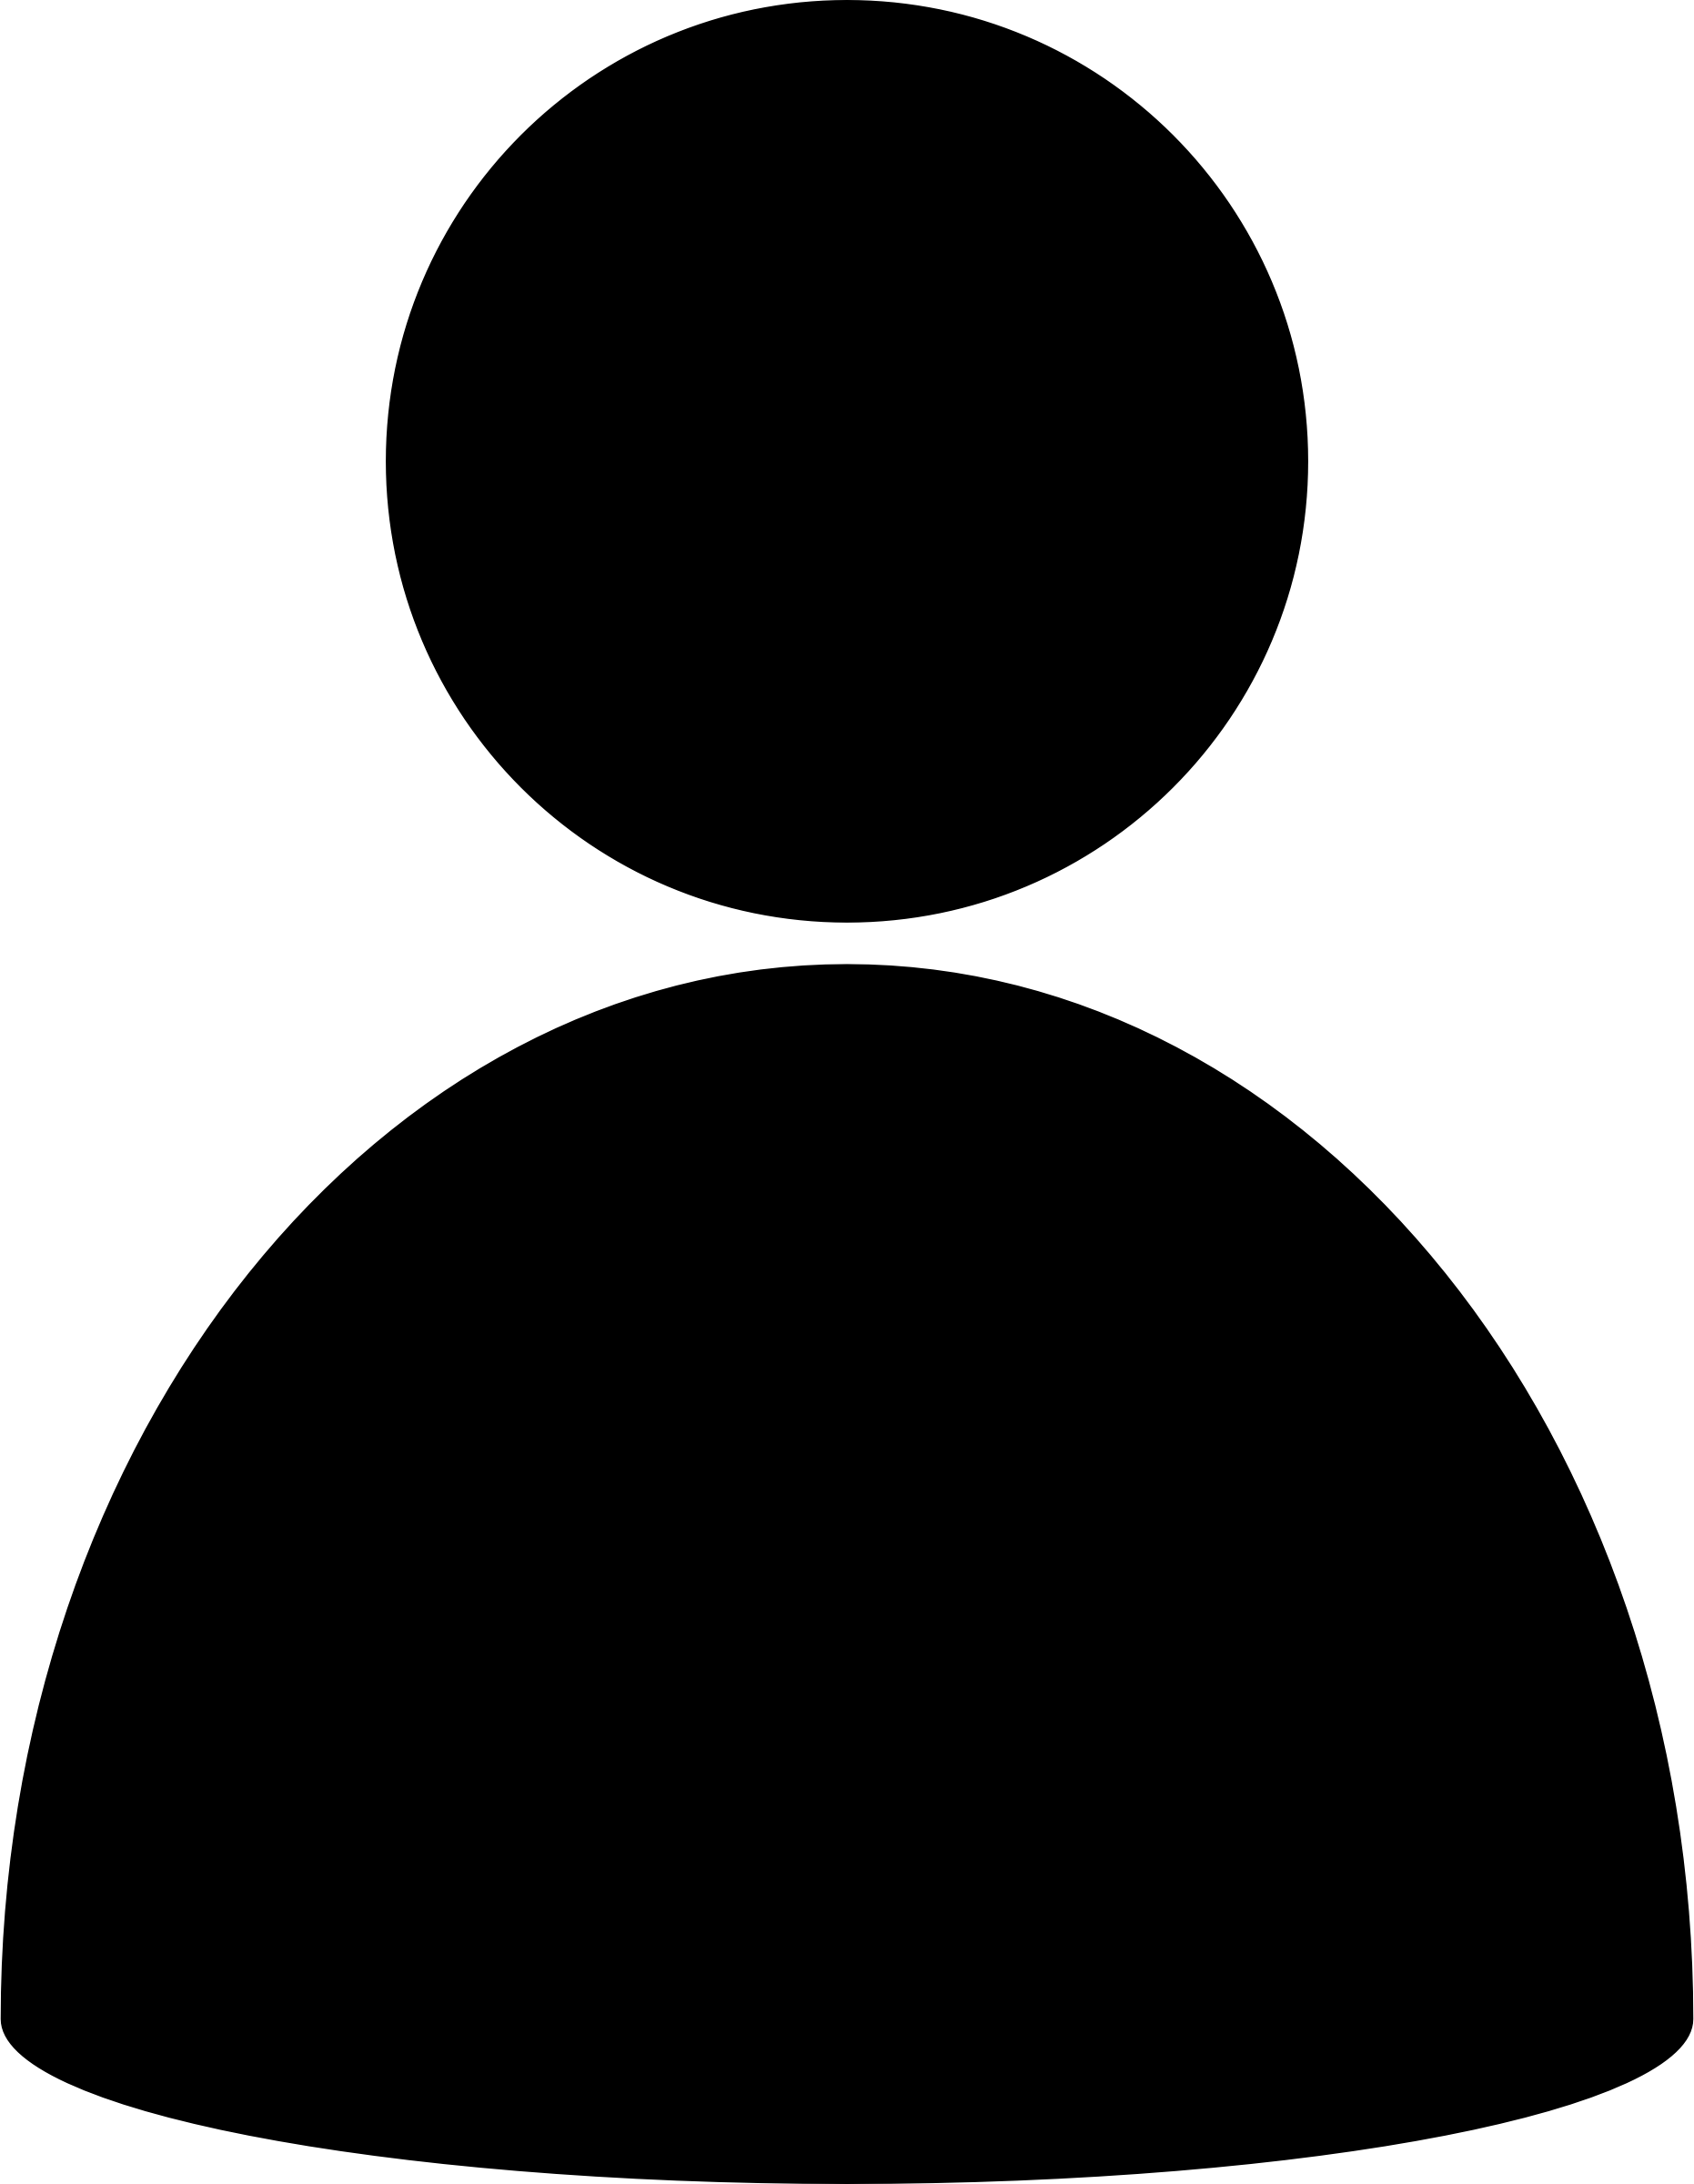
\includegraphics[height=\pht]{stock/person}};
      \node at (a.south) [label] {\Large a};
      }
      \uncover<4->{
      \node (c) [below left=0.25 and 0.25 of cd] {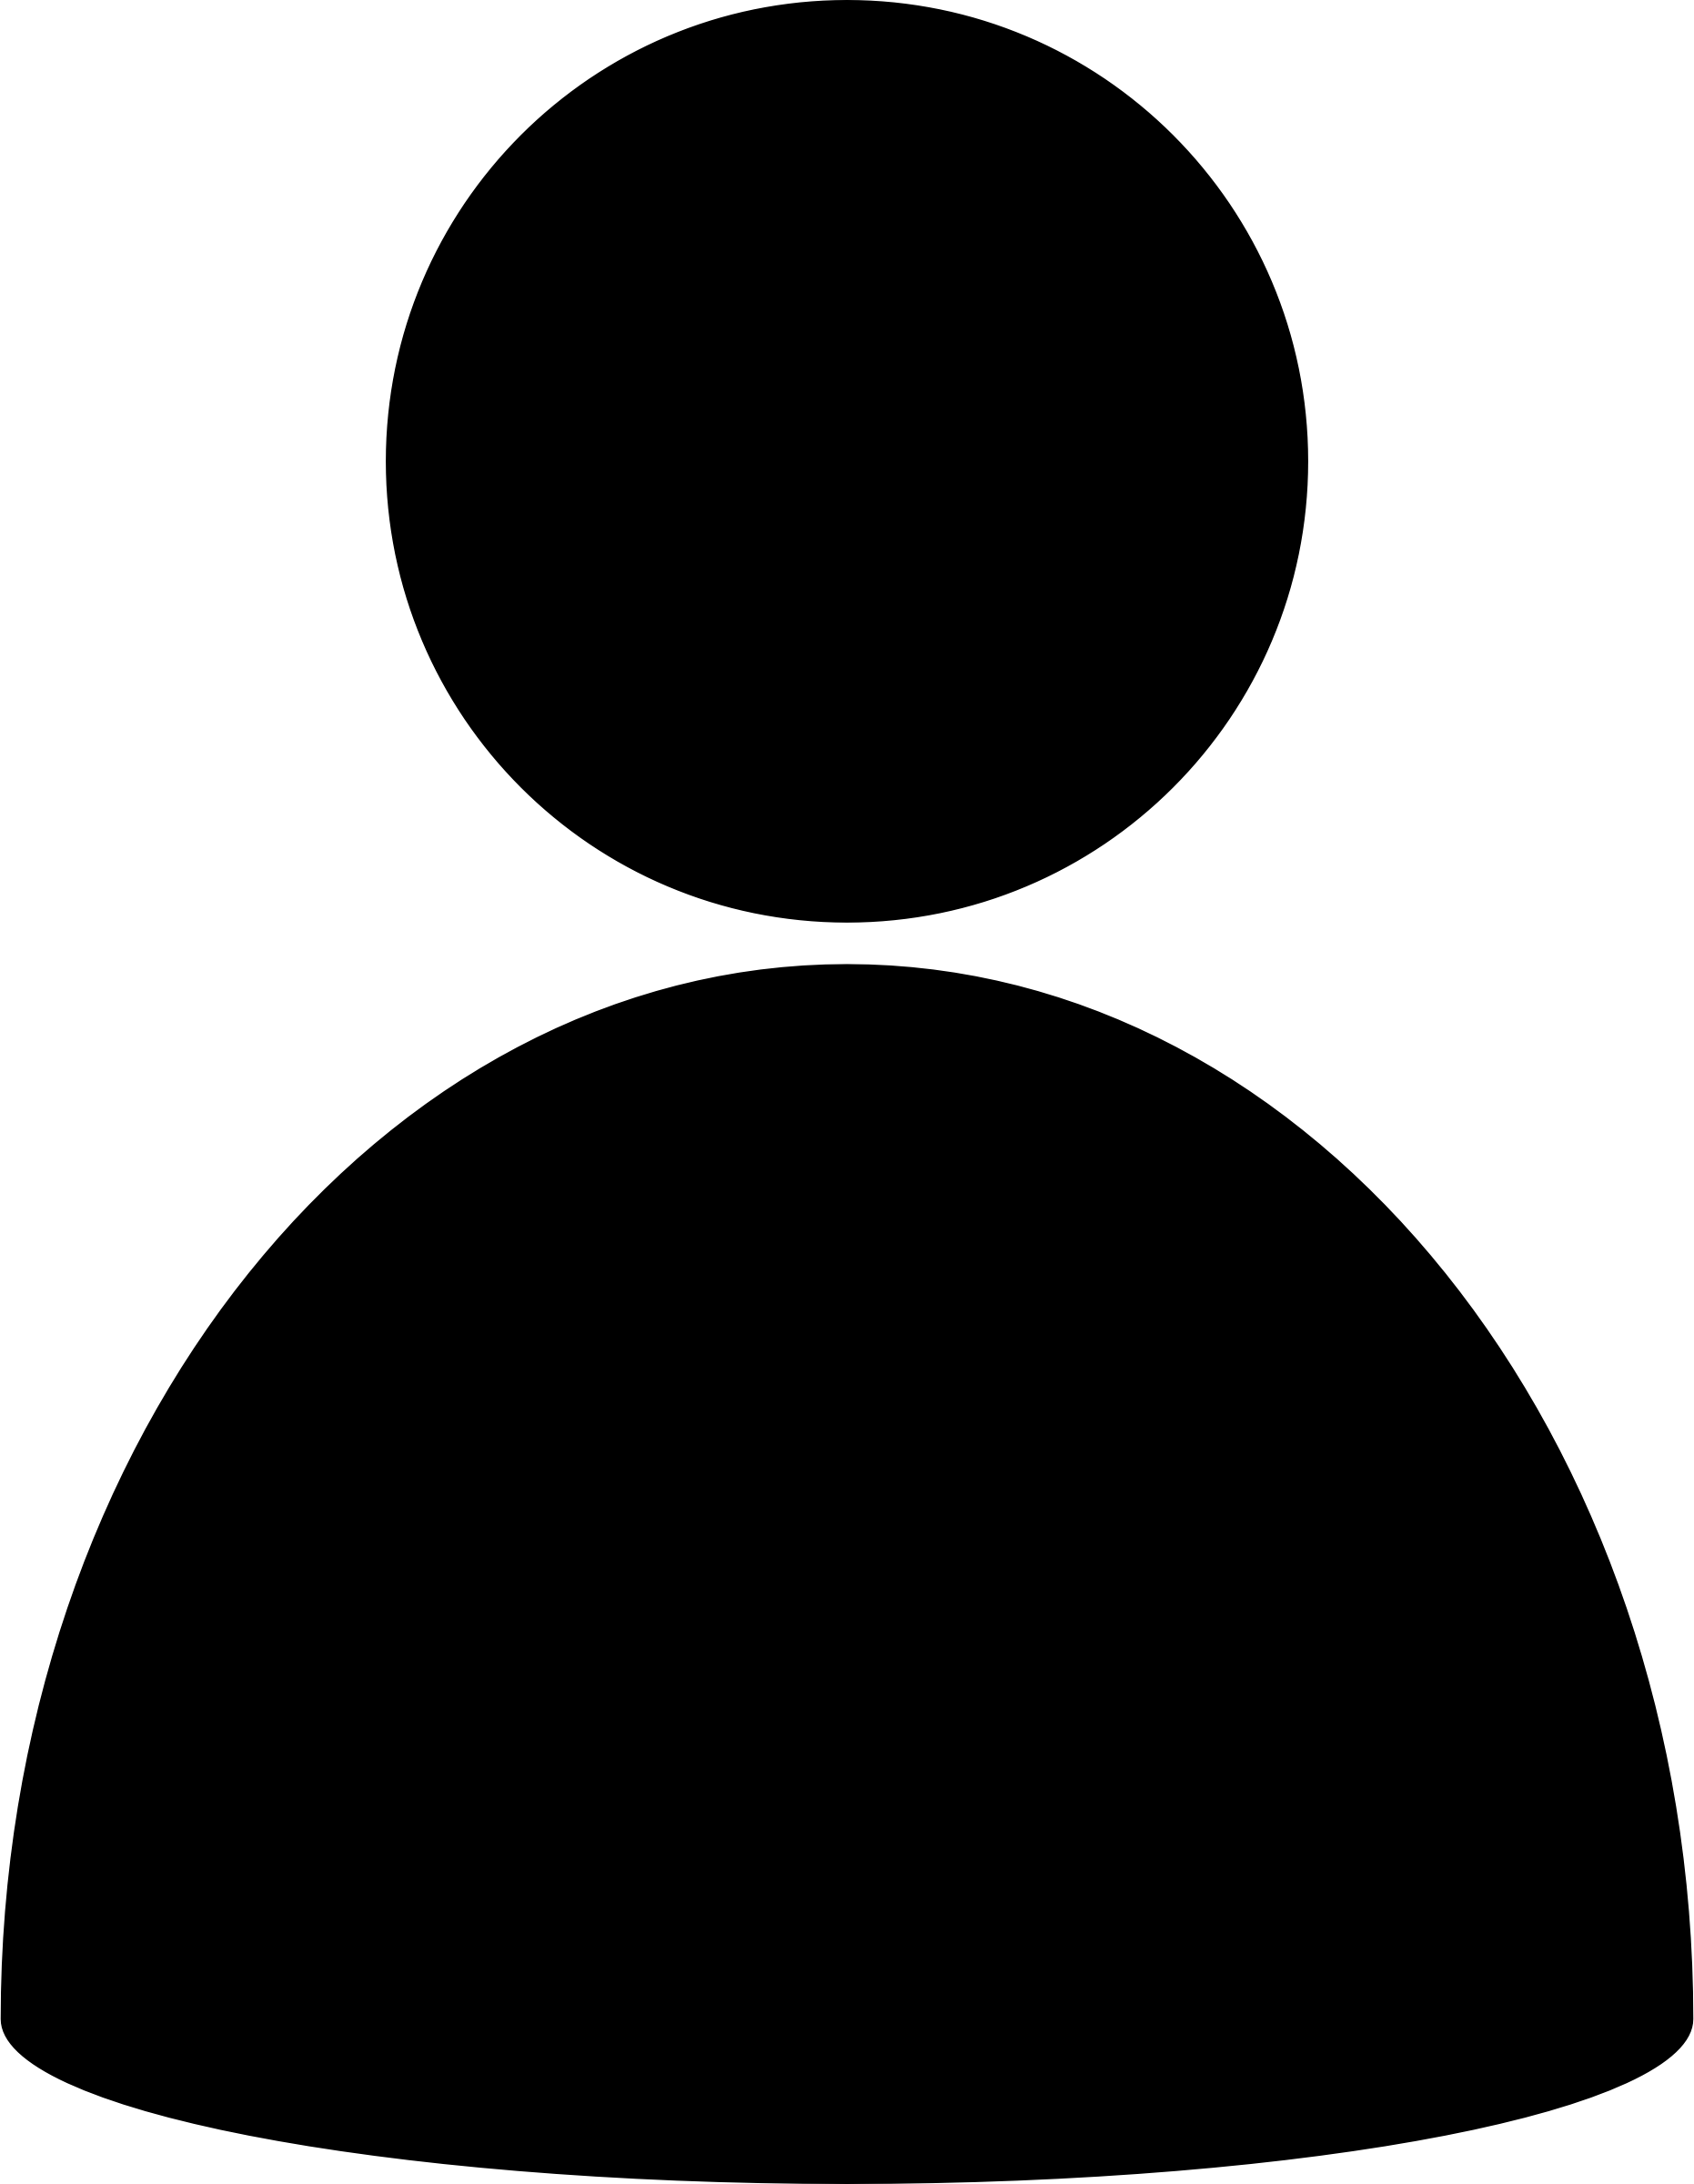
\includegraphics[height=\pht]{stock/person}};
      \node at (c.south) [label] {\Large c};
      \node (d) [below right=0.4 and 0.4 of cd] {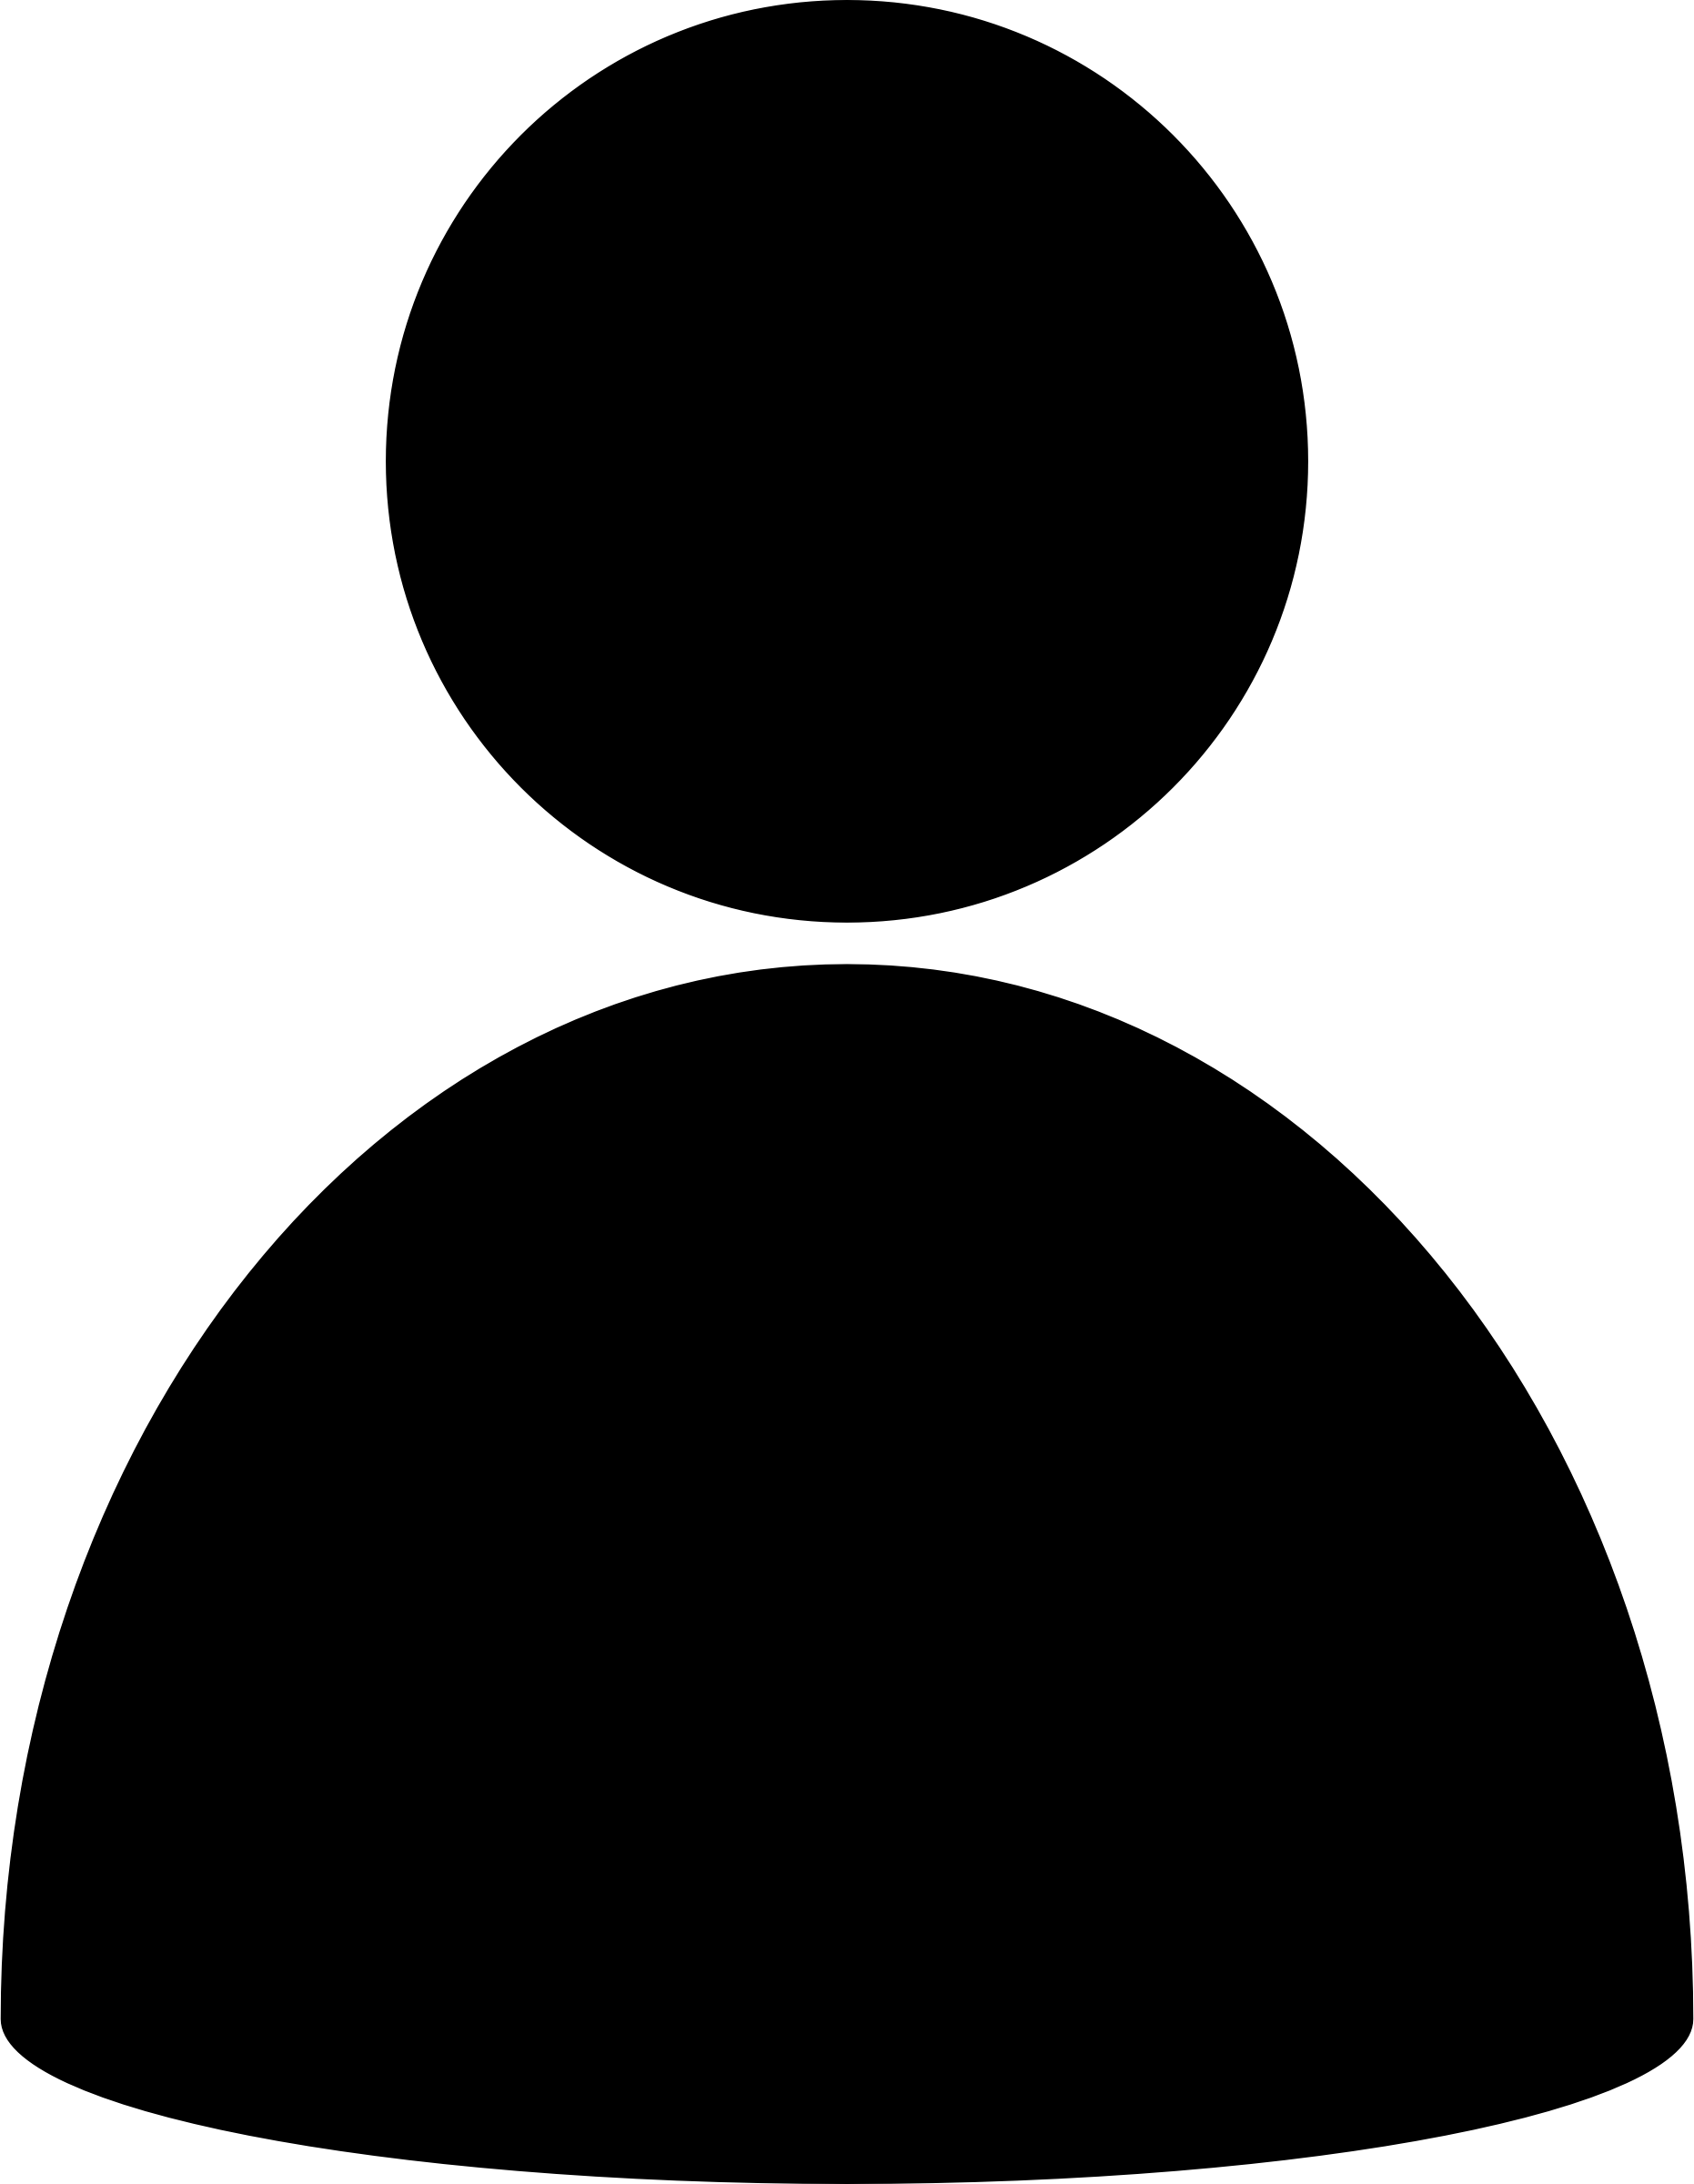
\includegraphics[height=\pht]{stock/person}};
      \node at (d.south) [label] {\Large d};
      }
    
      \uncover<2->{
      \draw [red] (abcd) -- (b);
      \draw [-, dashed] (abcd) -- (acd);
      }
      \uncover<3->{
      \draw [blue] (acd) -- (cd);
      \draw [-, dashed] (acd) -- (a);
      }
      \uncover<4->{
      \draw [-, dashed] (cd) -- (c);
      \draw [green!80!black] (cd) -- (d);
      }
    \end{tikzpicture}

  $\qquad$contact network \hfill transmission tree$\qquad$
  \end{center}
\end{frame}

\begin{frame}{Transmission trees shape viral phylogenies}
  some demo of viruses evolving and being transmitted at the same time
\end{frame}

\begin{frame}{Can we fit network models with viral phylogenies?}
  \begin{center}
  network $\to$ transmission tree $\to$ viral phylogeny \\
  \hfill\\
  network $\stackrel{\alert{?}}{\leftarrow}$ transmission tree $\leftarrow$ viral phylogeny \\
  \end{center}
\end{frame}

\begin{frame}{Are network parameters identifiable from tree shape?}
  \begin{minipage}[p][\textheight][t]{\textwidth}
    \only<1>{\includegraphics[width=0.9\textwidth, trim=0 3in 0 0, clip]{kernel-idea.pdf}}
    \only<2>{\includegraphics[width=0.9\textwidth, trim=0 1.7in 0 0, clip]{kernel-idea.pdf}}
    \only<3>{\includegraphics[width=0.9\textwidth, trim=0 0.8in 0 0, clip]{kernel-idea.pdf}}
    \only<4->{\includegraphics[width=0.9\textwidth, trim=0 0in 0 0, clip]{kernel-idea.pdf}}
  \end{minipage}
\end{frame}

\begin{frame}{yes they do}
  \centerline{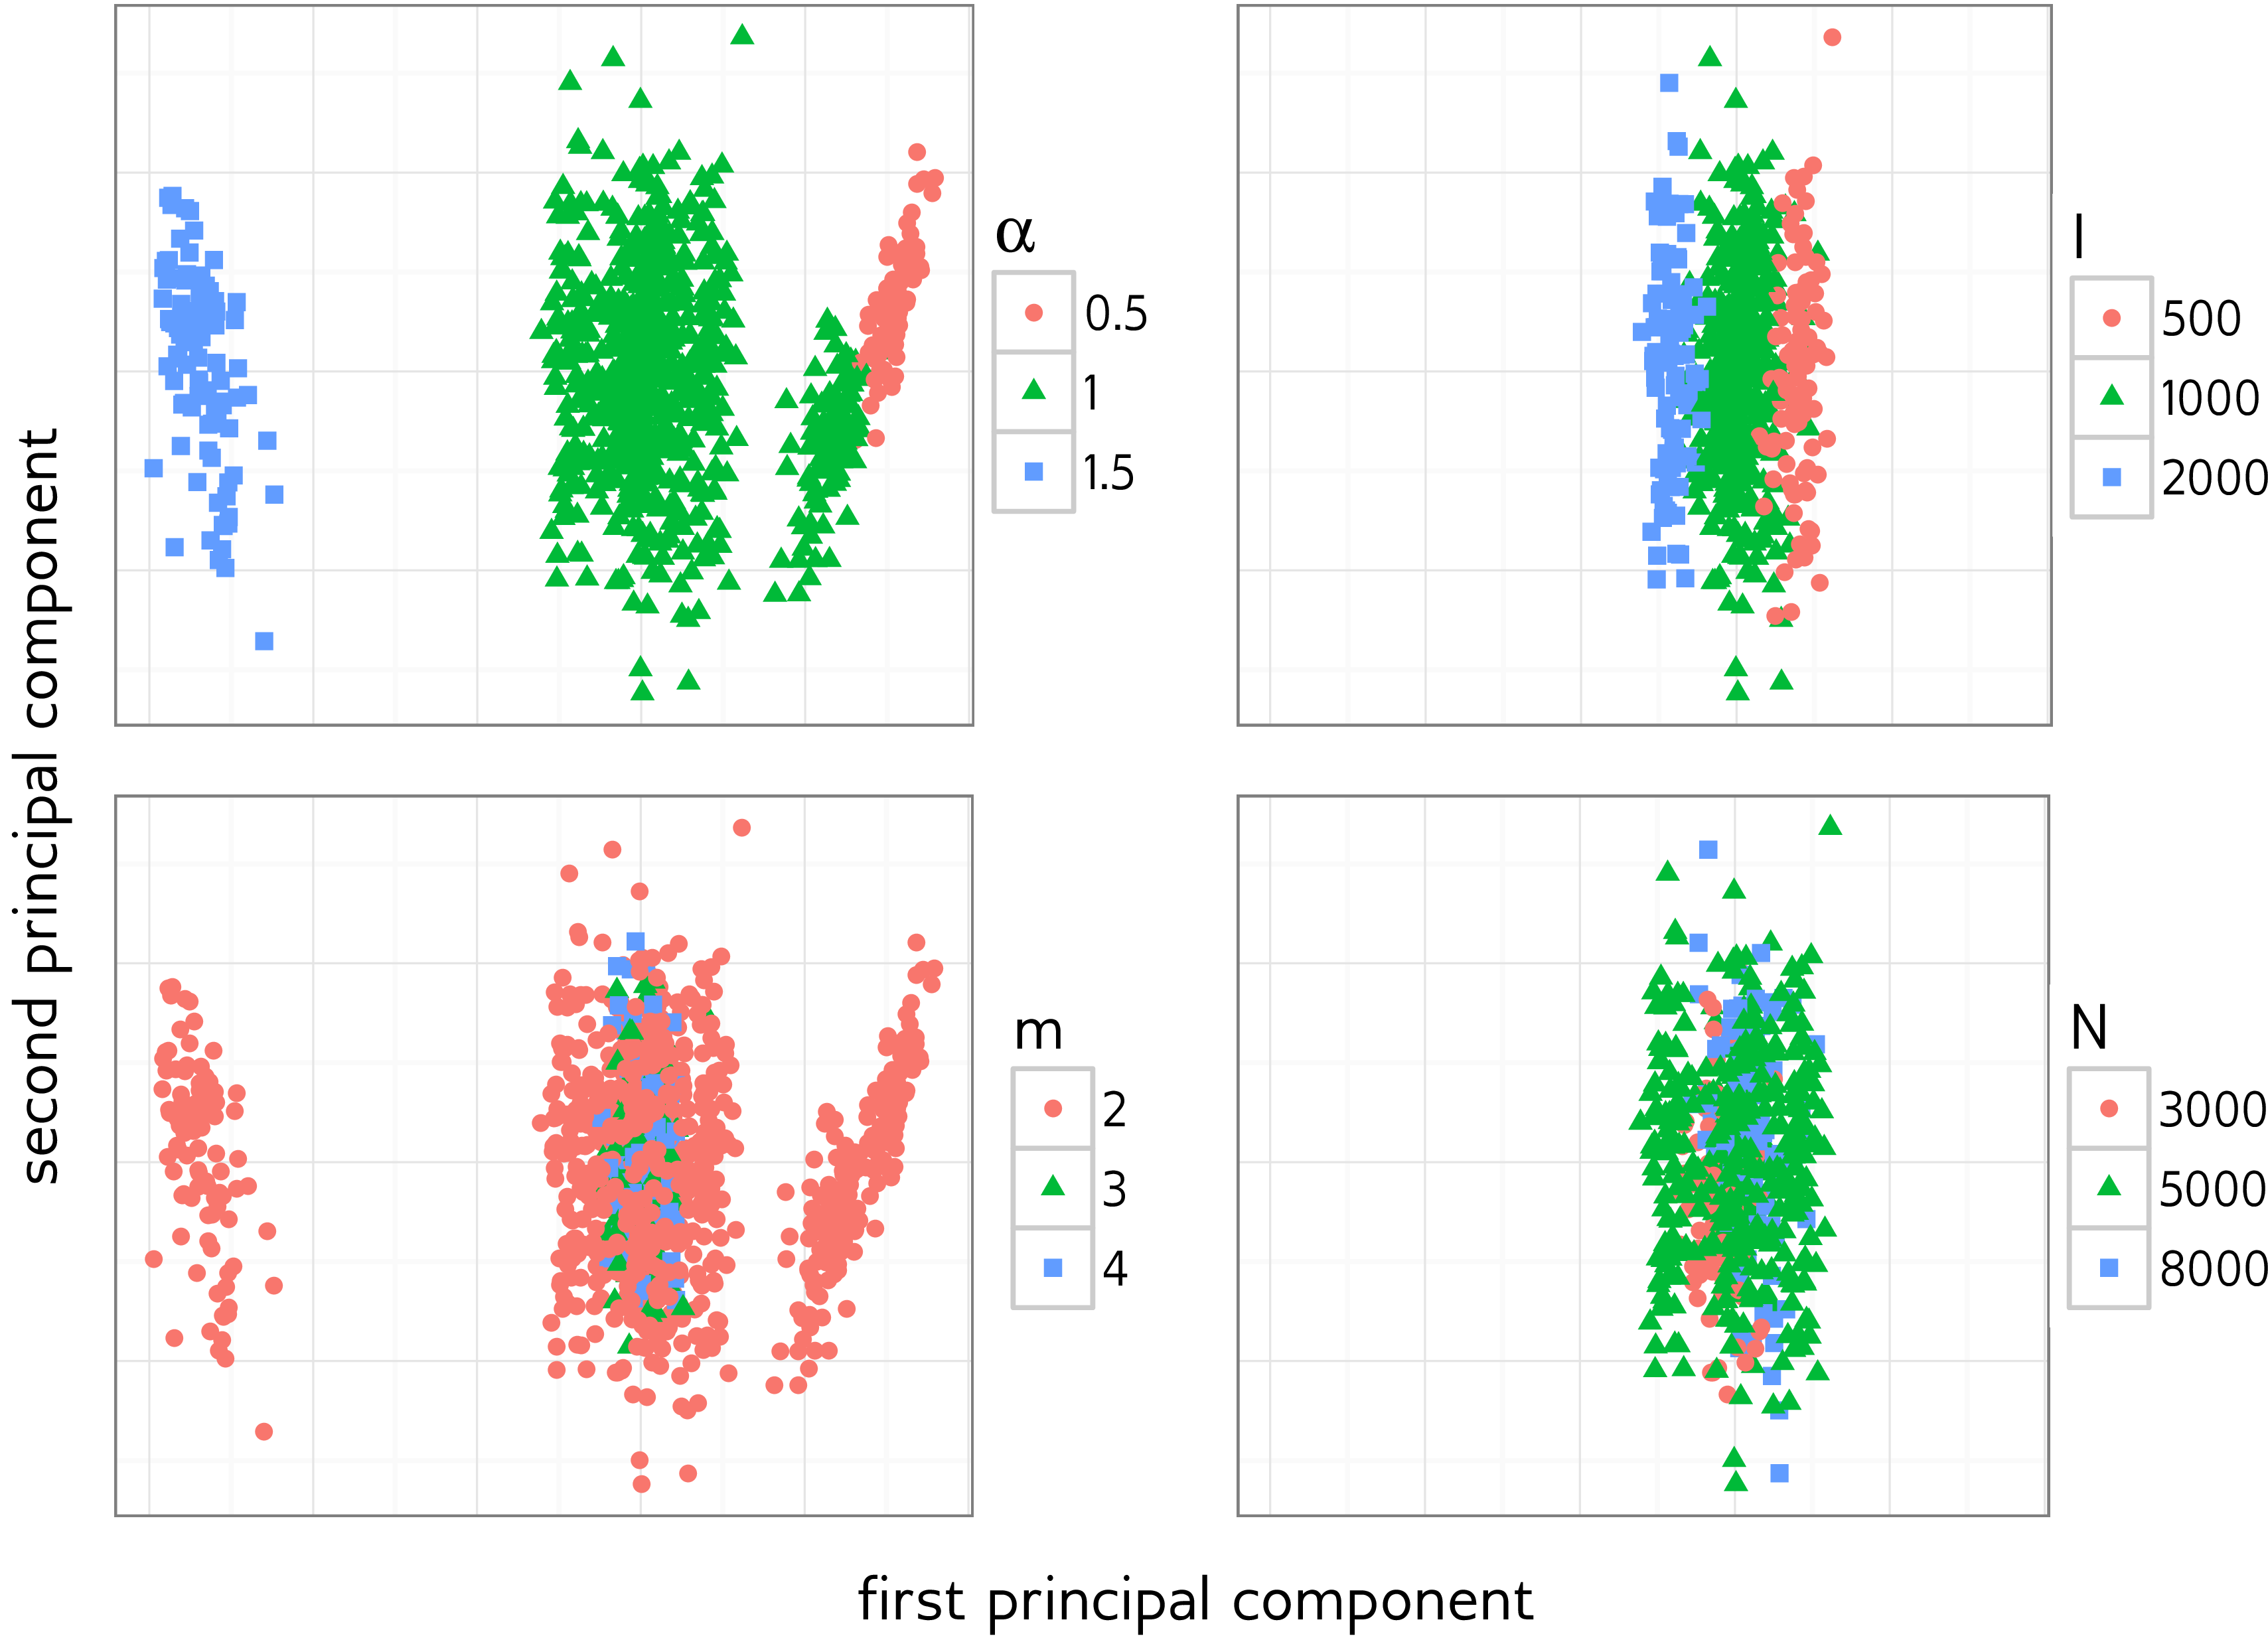
\includegraphics[height=0.8\textheight]{kernel-kpca}}
\end{frame}

\begin{frame}{Simulated trees can be used to fit network models}
  \centerline{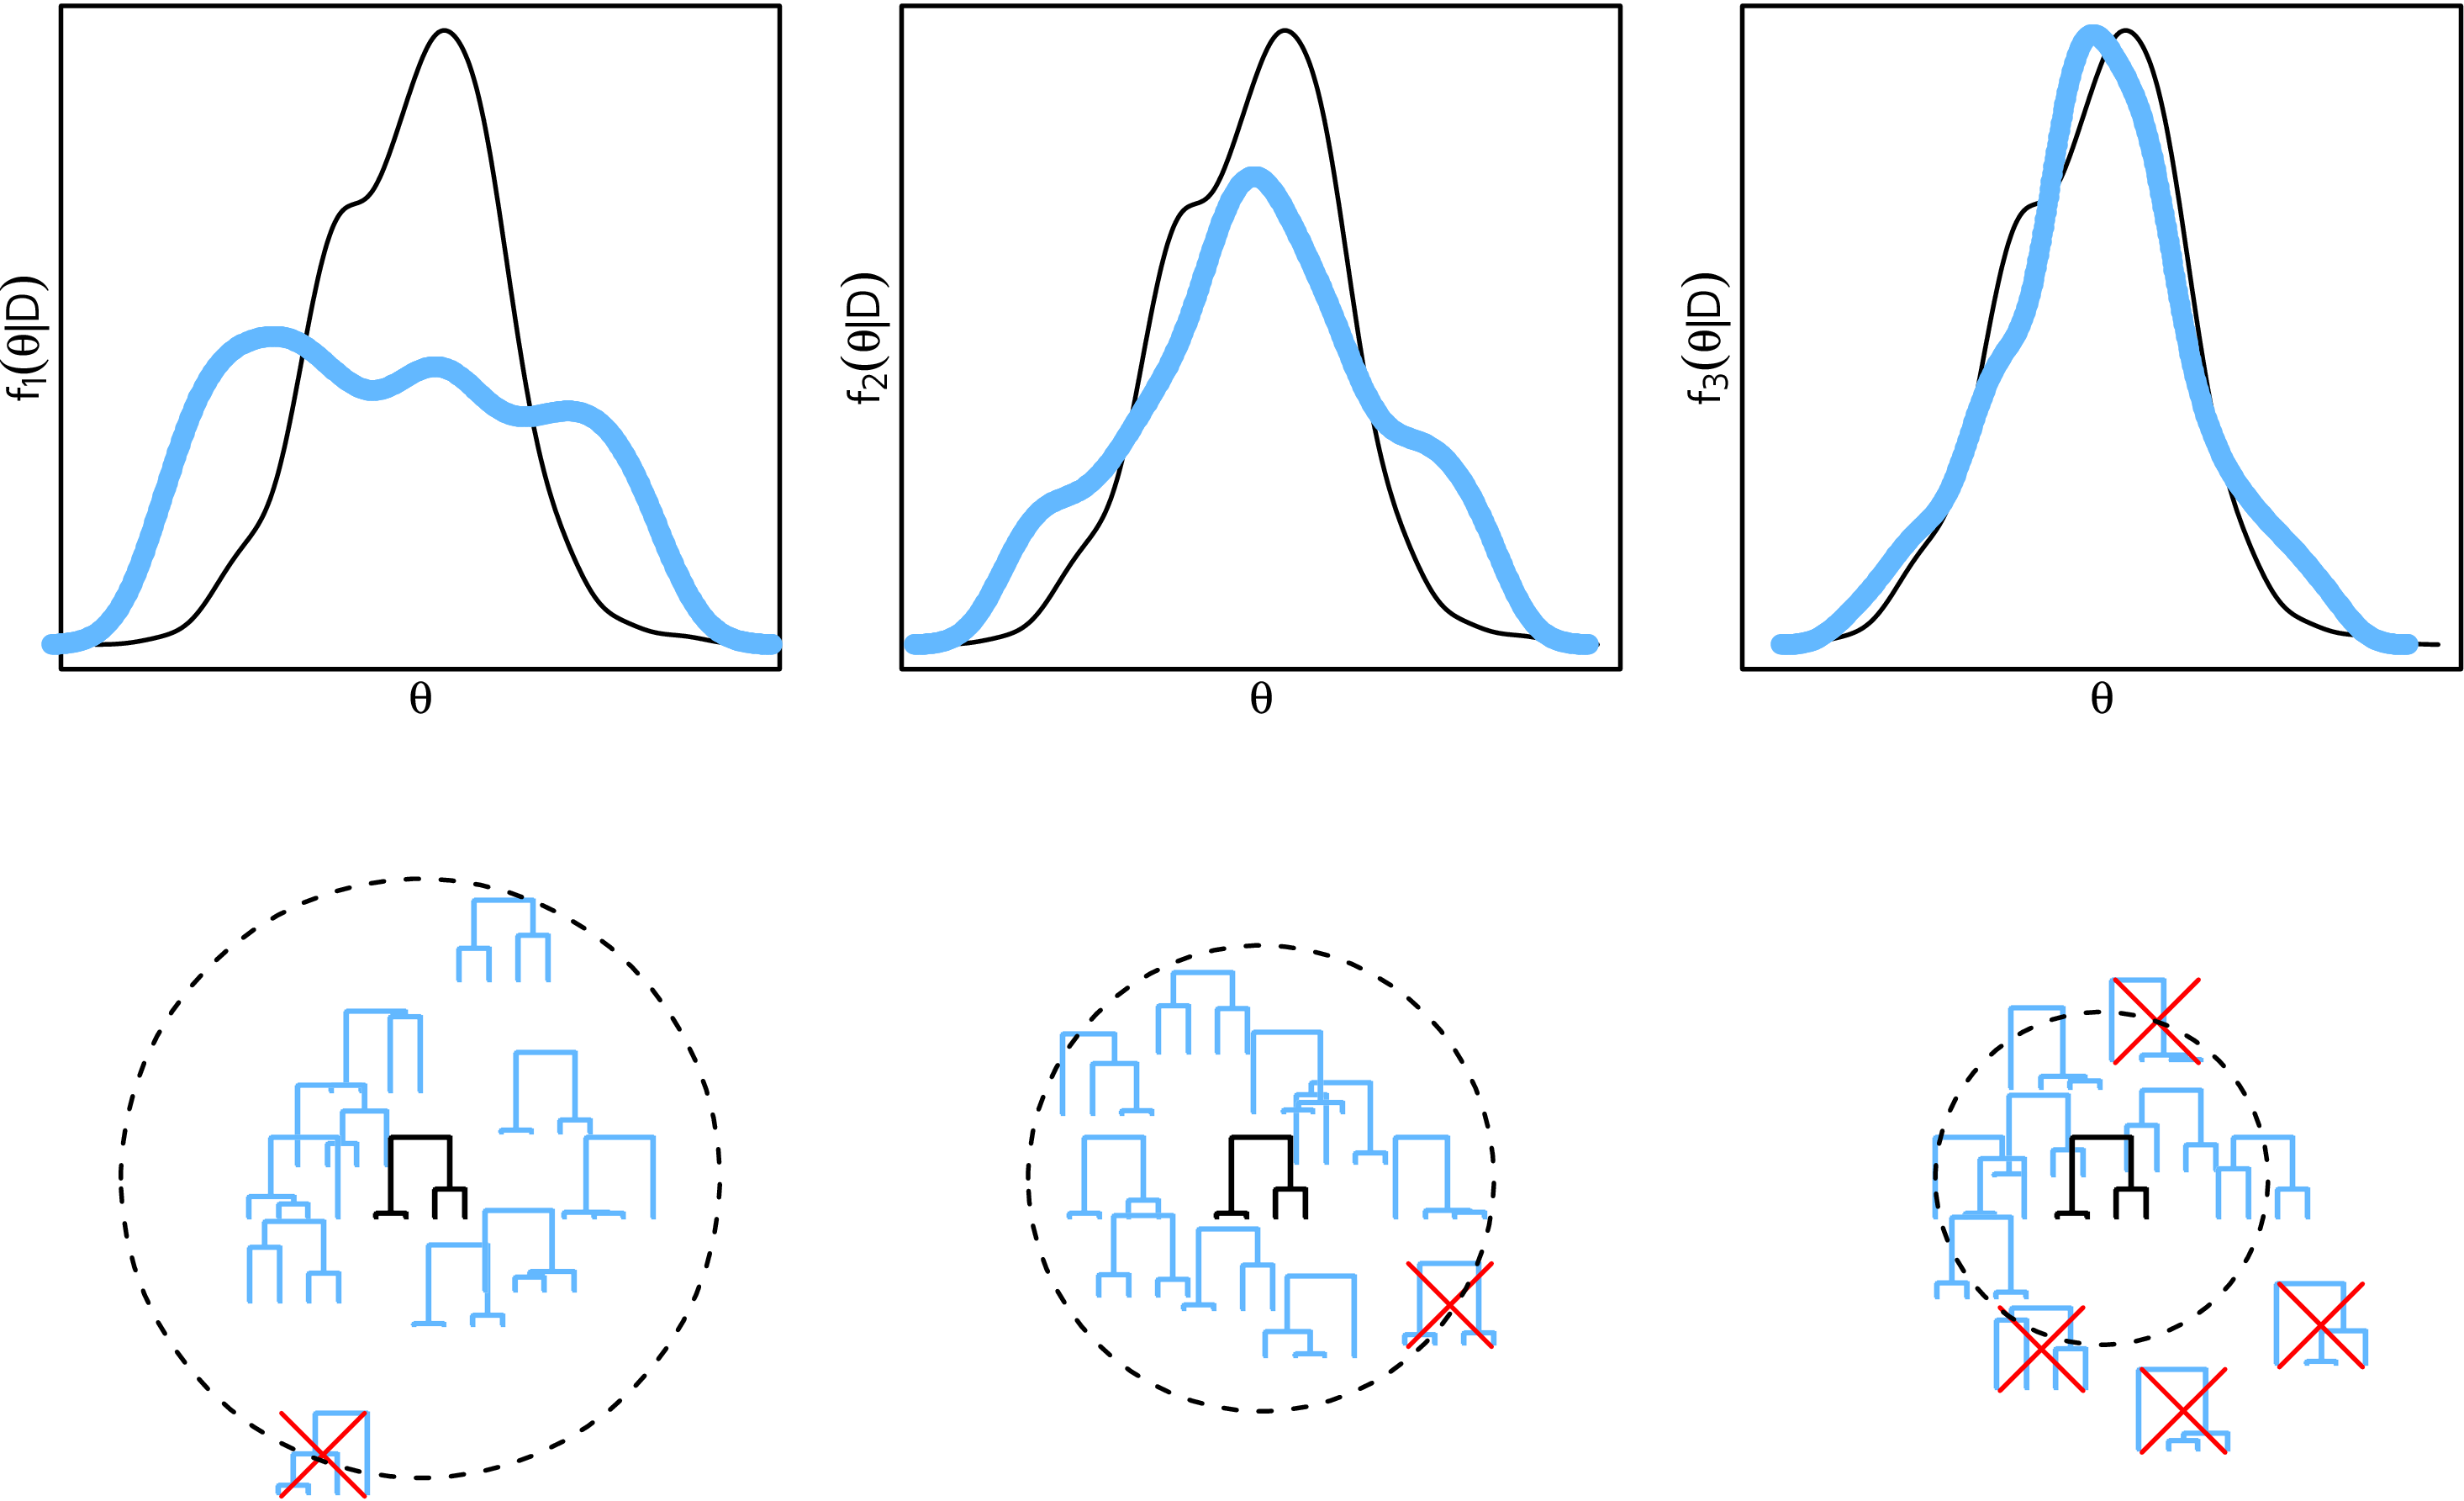
\includegraphics[width=0.9\textwidth]{abc-smc}}

  \centerline{animate this?}
\end{frame}

\begin{frame}{Posterior mean estimates are more accurate for $\alpha$ and $I$}
  \begin{minipage}[p][\textheight][t]{\textwidth}
    \vspace{-0.5cm}
    preferential attachment power \hfill \uncover<2>{edges per vertex}

    \hspace{0.75cm}\only<1>{\includegraphics[height=0.8\textheight, trim=0 0 3.4in 0, clip]{abc-point-estimate-m3.pdf}}
    \only<2>{\includegraphics[height=0.8\textheight]{abc-point-estimate-m3.pdf}}

    prevalence \hfill \uncover<2>{total nodes}
  \end{minipage}
\end{frame}

\begin{frame}{Example simulation\ldots}
  \begin{minipage}[p][\textheight][t]{\textwidth}
    \begin{center}
    preferential attachment power \hfill prevalence
    \only<1>{
      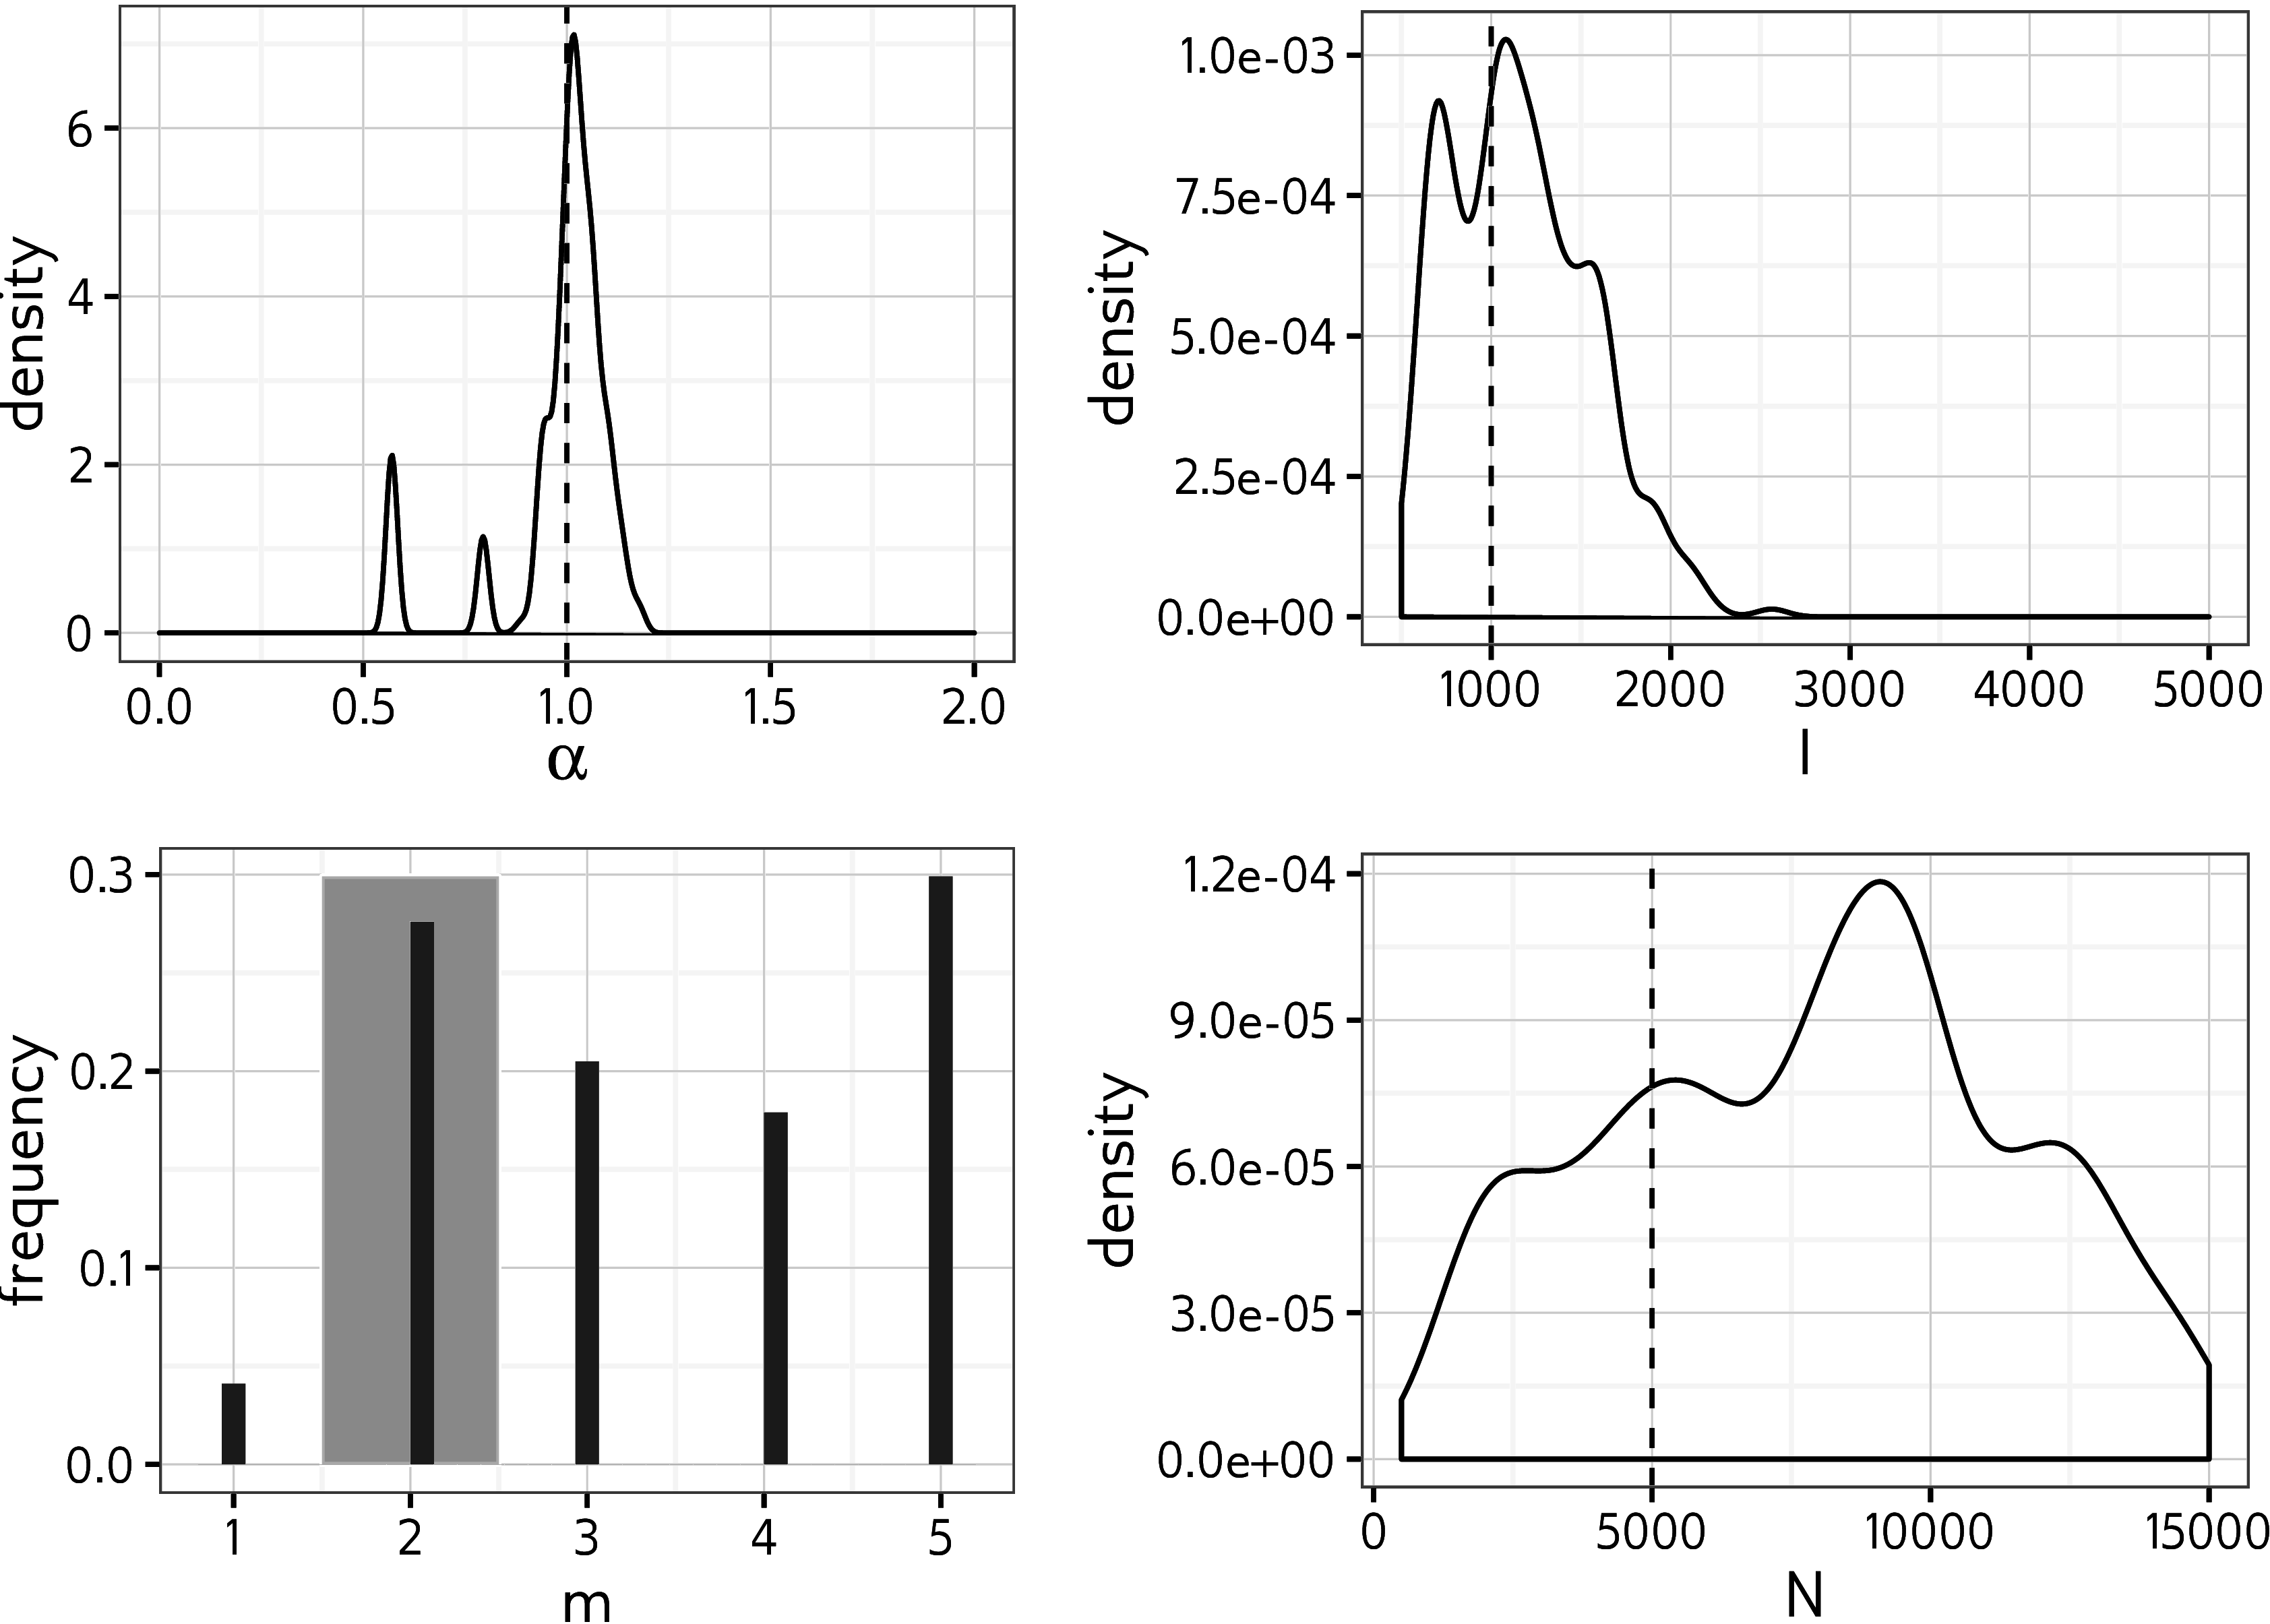
\includegraphics[width=0.8\textwidth, trim=0 2.5in 0 0, clip]{abc-posterior-example.pdf}
    }
    \only<2>{
      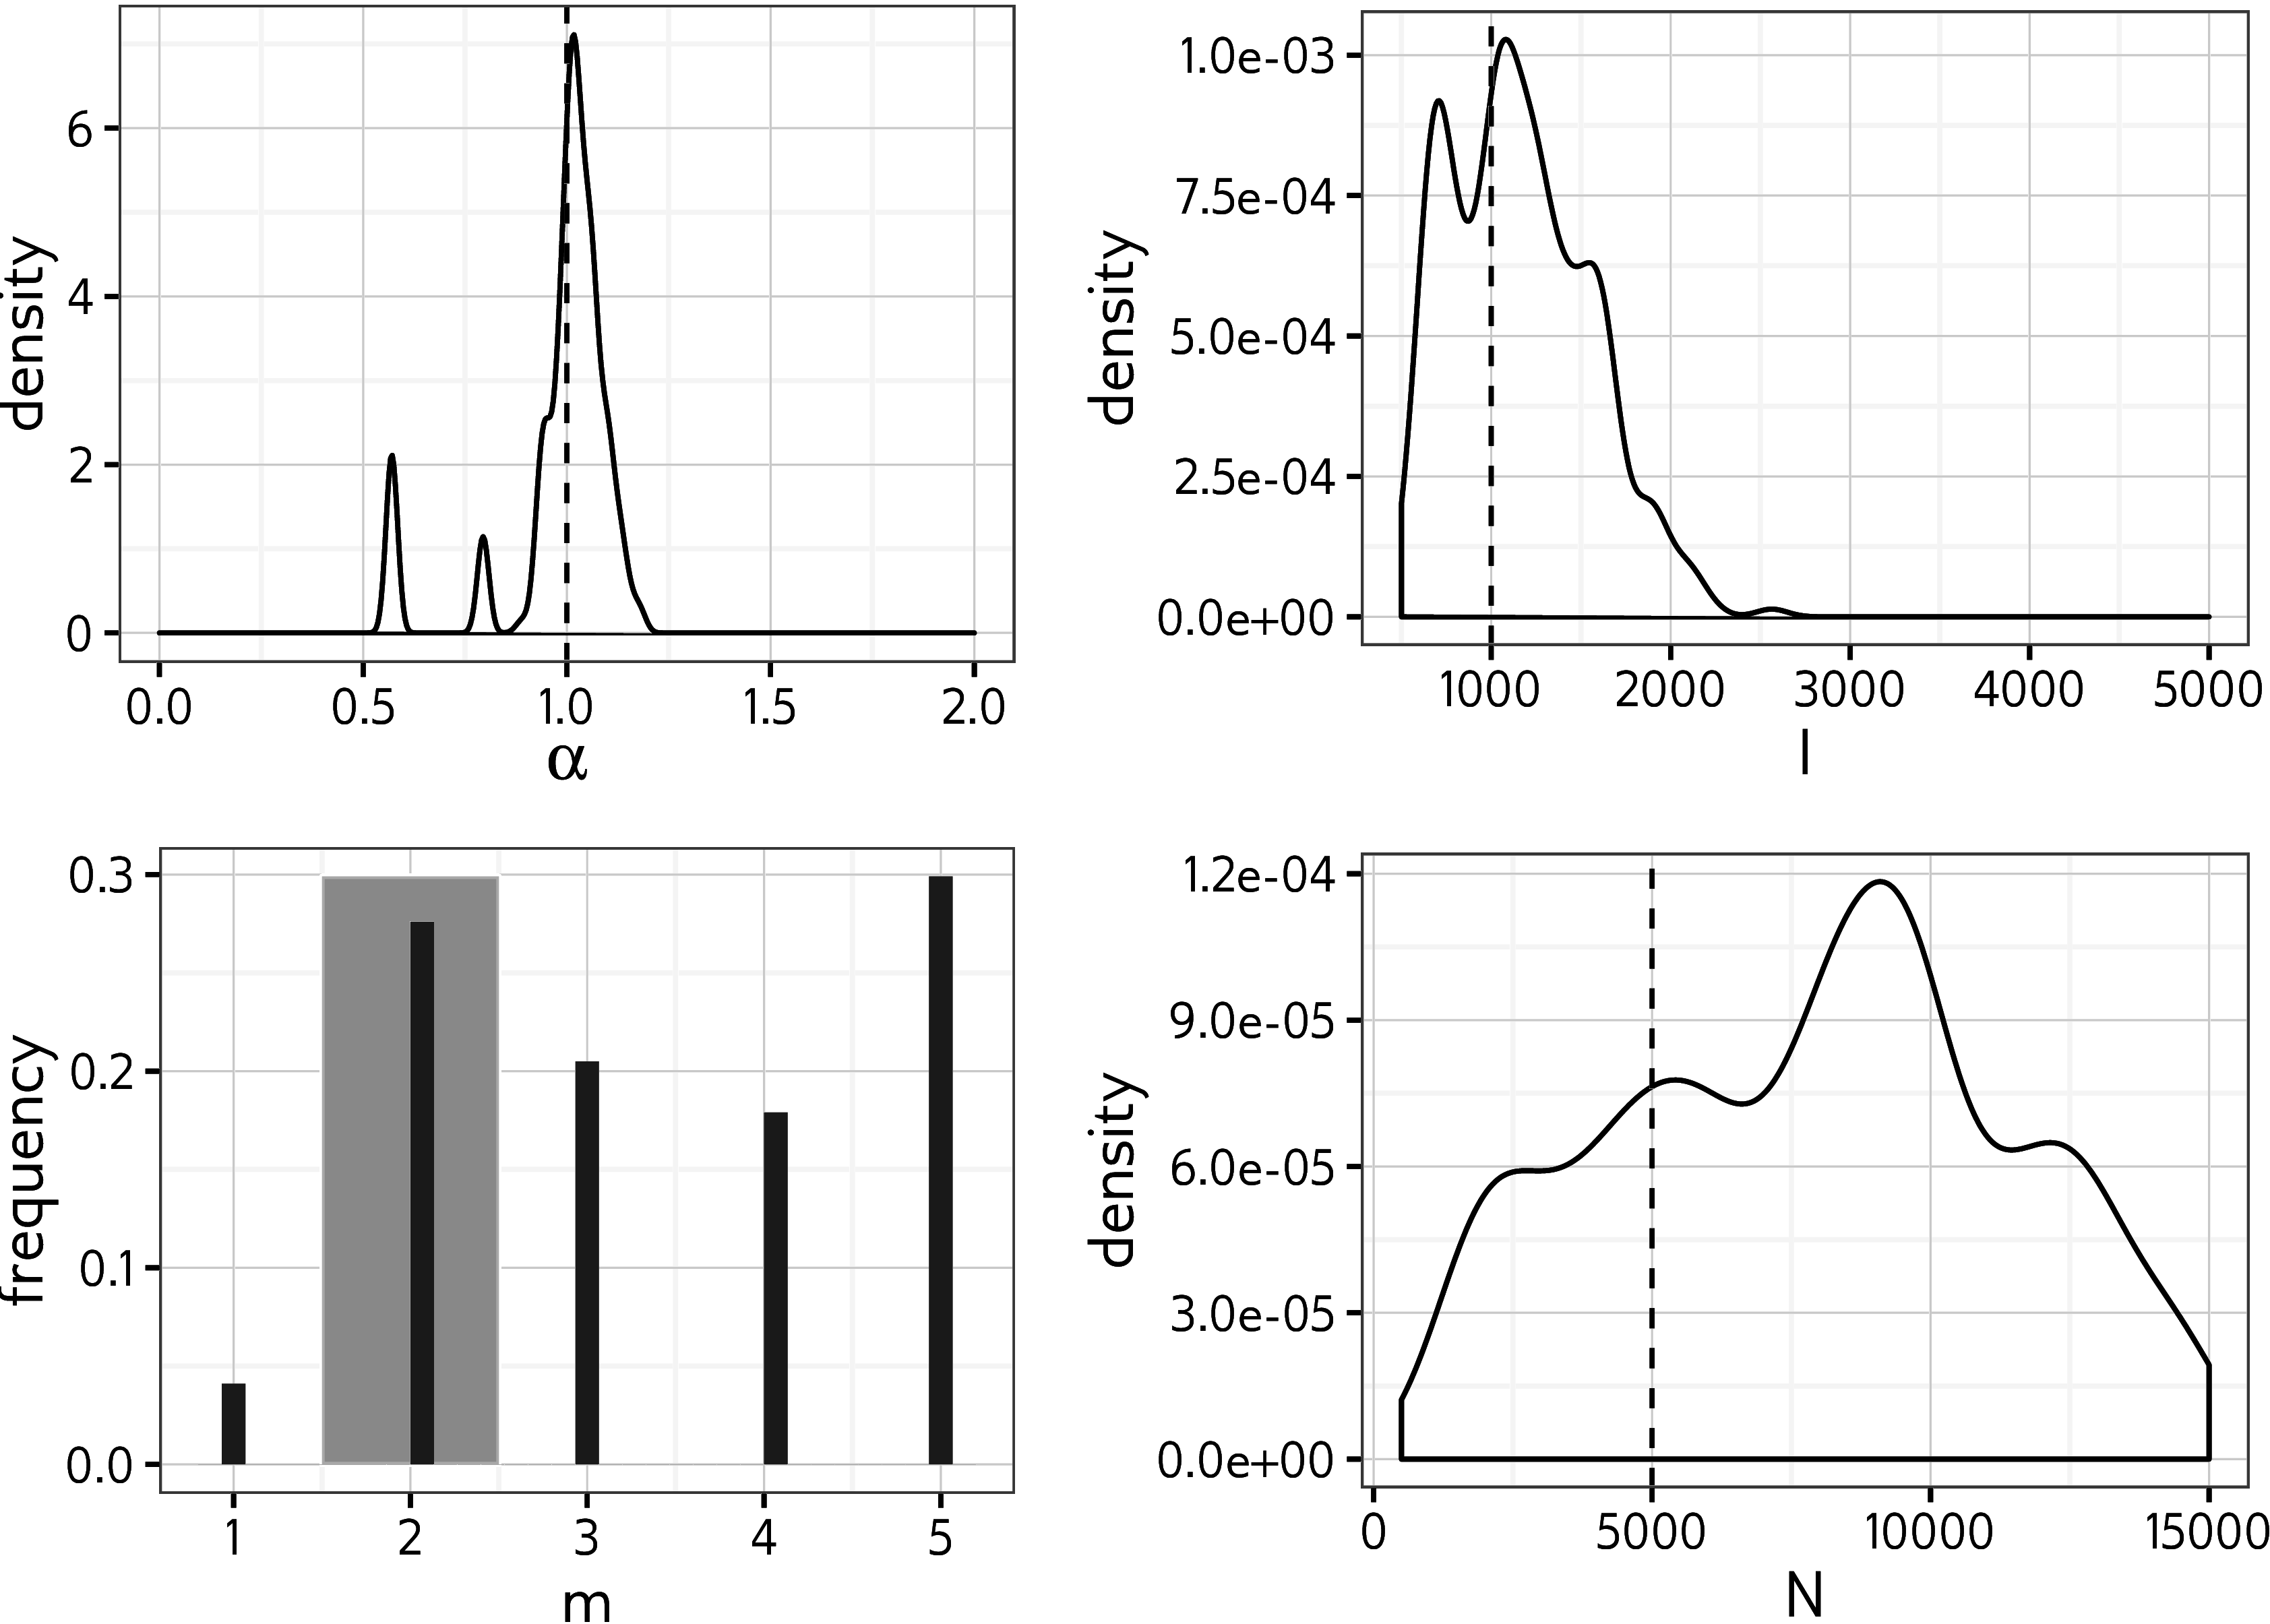
\includegraphics[width=0.8\textwidth]{abc-posterior-example.pdf}

      \vspace{-0.25cm}
      edges per vertex \hfill total nodes
    }
    \end{center}
  \end{minipage}
\end{frame}

\begin{frame}{Example simulation continued, $N$ and $I$ confounded}
  %\includegraphics[width=\textwidth]{{abc-posterior-2d/1.0_1000_3_5000_0}.pdf}
\end{frame}

\begin{frame}{Application to real world HIV datasets}
  \centerline{\begin{tabular}{ccc}
  Dataset & Sequences ($n$) & Gene \\
  \hline
  IDU/Estonia~\autocite{zetterberg2004two} & 171/188 & \textit{env}/\textit{gag} \\
  IDU/Romania~\autocite{niculescu2015recent} & 136 & \textit{pol} \\
  IDU/Canada & 399 & \textit{pol} \\
  HET/Botswana~\autocite{novitsky2013phylogenetic,novitsky2014impact} & 180 & \textit{env} \\
  HET/Malawi~\autocite{mccormack2002early} & 141/154 & \textit{env}/\textit{gag} \\
  HET/Uganda~\autocite{grabowski2014role} & 225 & \textit{env}/\textit{gag} \\
  MSM/Beijing~\autocite{wang2015targeting} & 173 & \textit{pol} \\
  MSM/Taiwan~\autocite{kao2011surveillance} & 275 & \textit{pol} \\
  MSM/USA~\autocite{little2014using} & 180 & \textit{pol} \\
  MSM/Shanghai~\autocite{li2015hiv} & 280 & \textit{pol} \\
  mixed/Spain~\autocite{cuevas2009hiv} & 287 & \textit{pol} \\
  \hline
\end{tabular}
}
\end{frame}

\begin{frame}{HIV networks have sub-linear preferential attachment}
    Also, higher PA for IDU networks.

    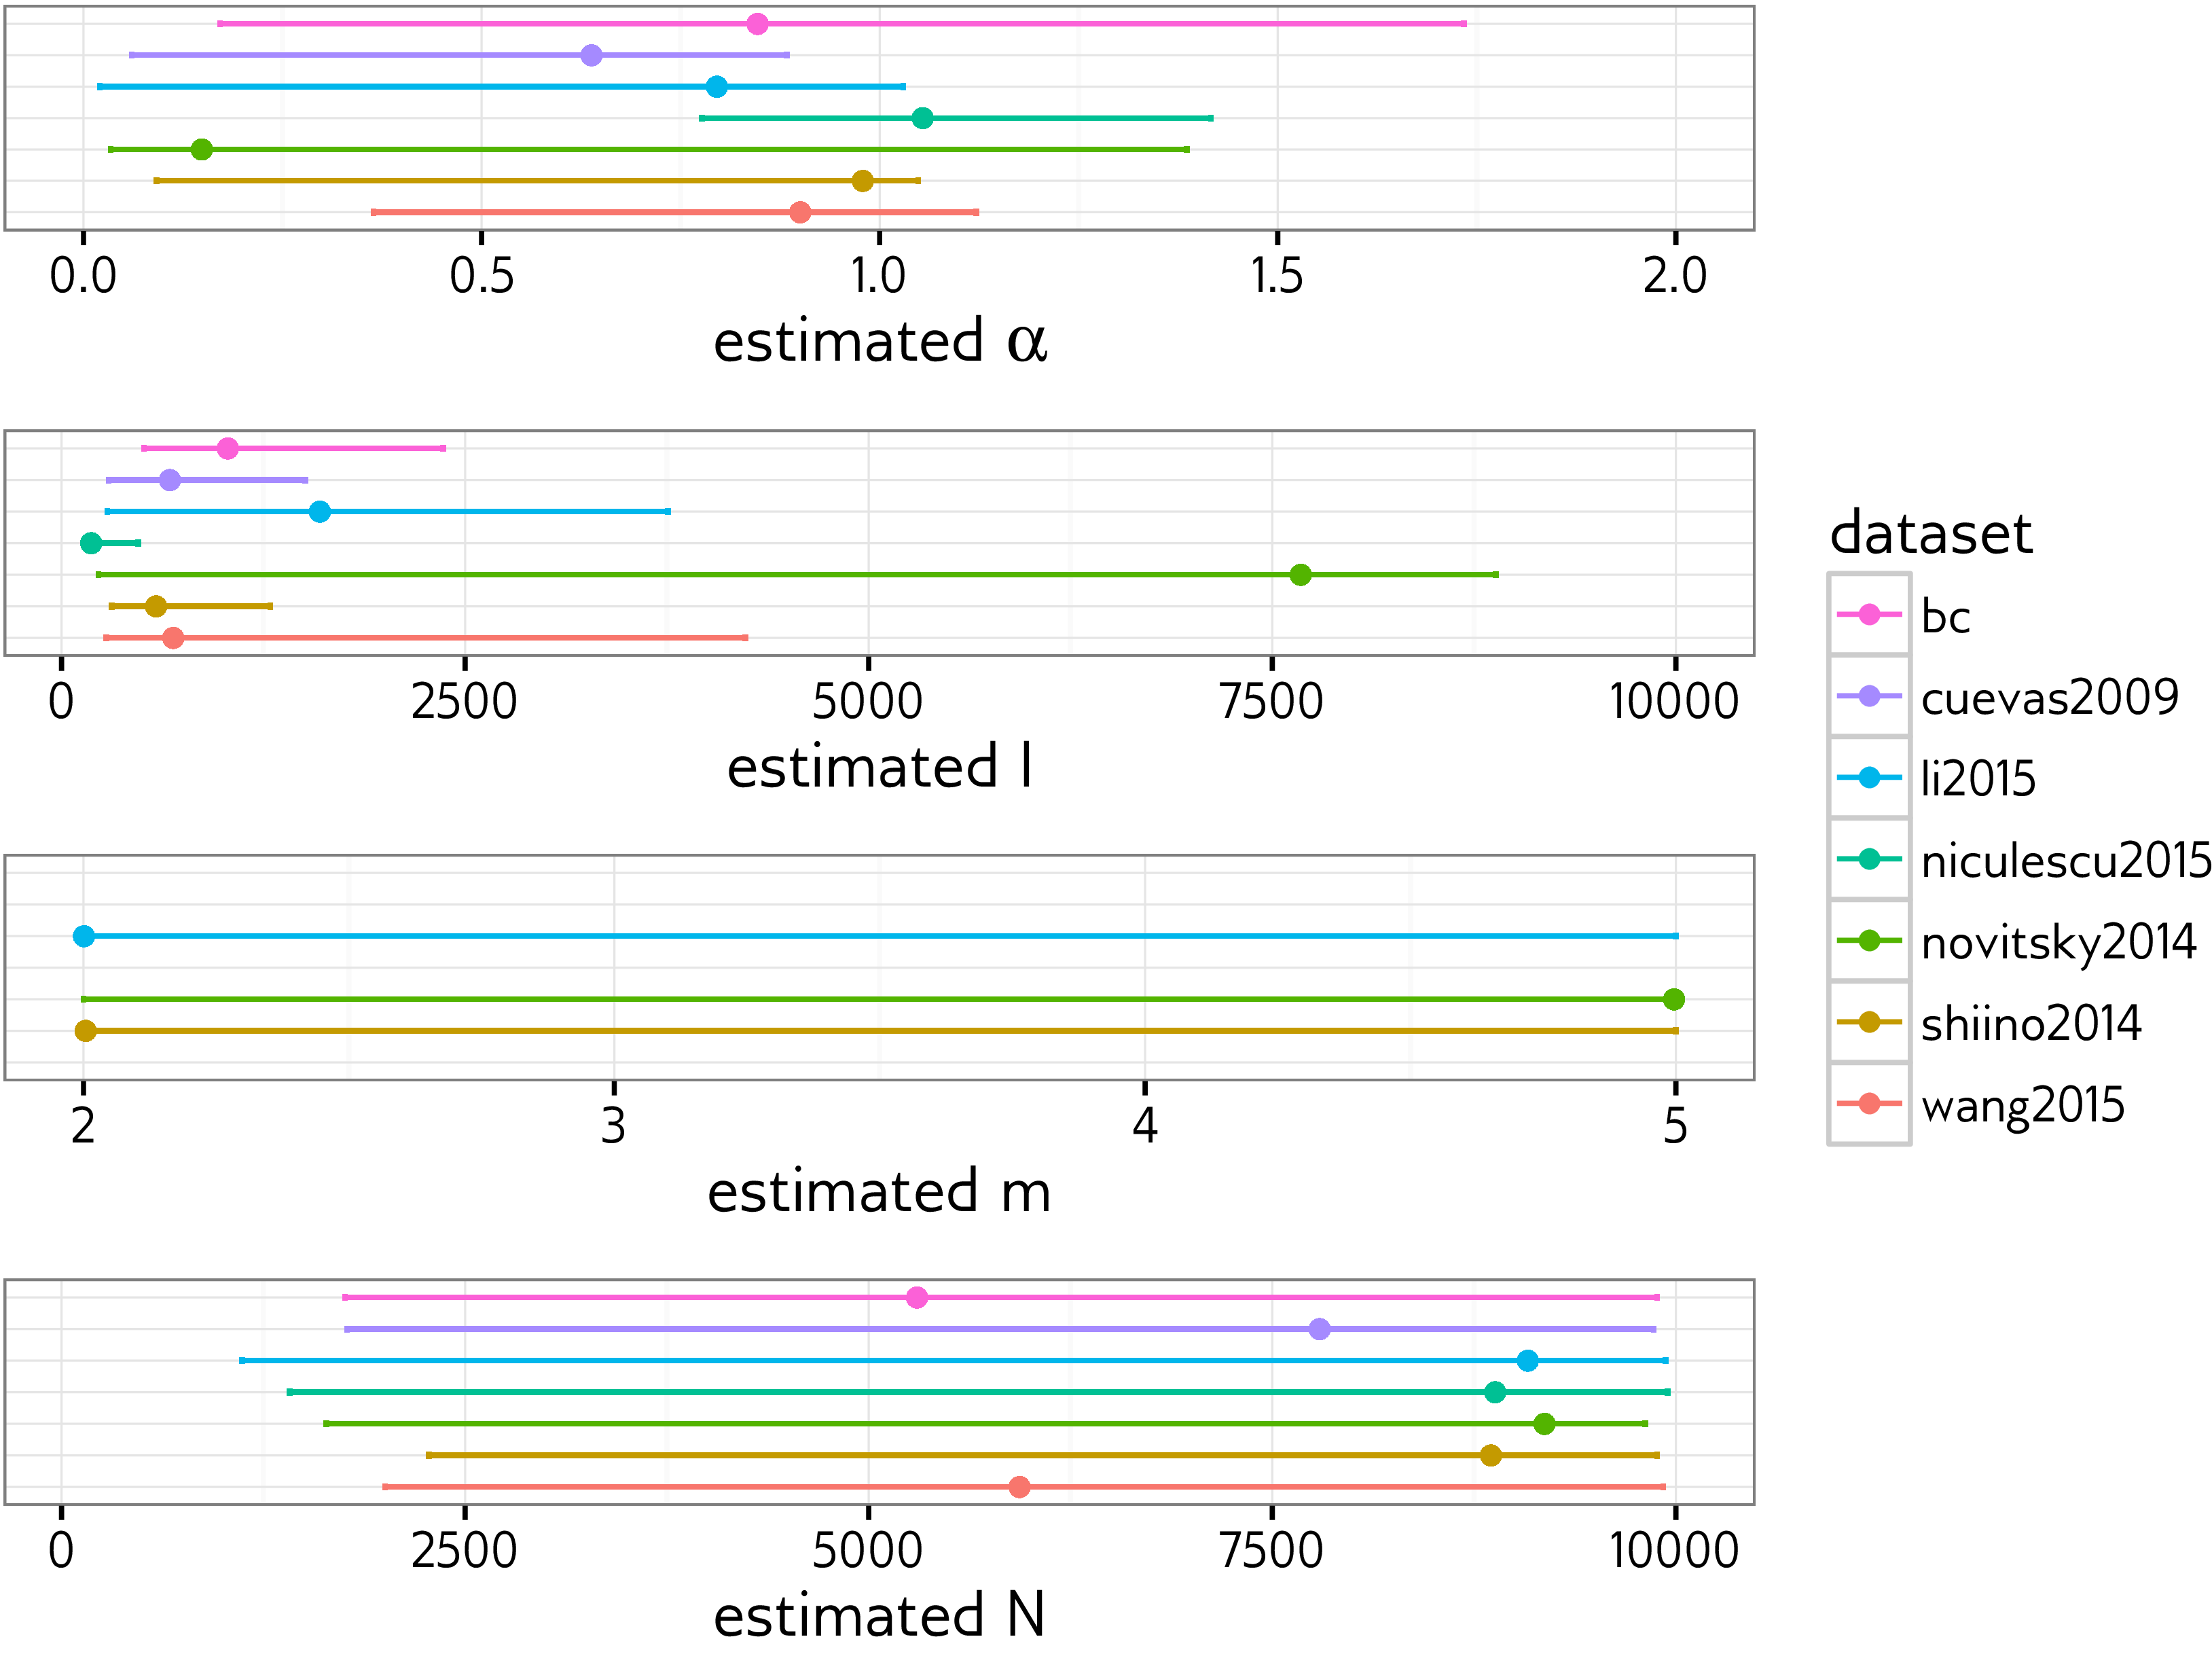
\includegraphics[trim=0 3.5in 3.3in 0, clip, width=0.5\textwidth]{realdata-hpd-bc}
    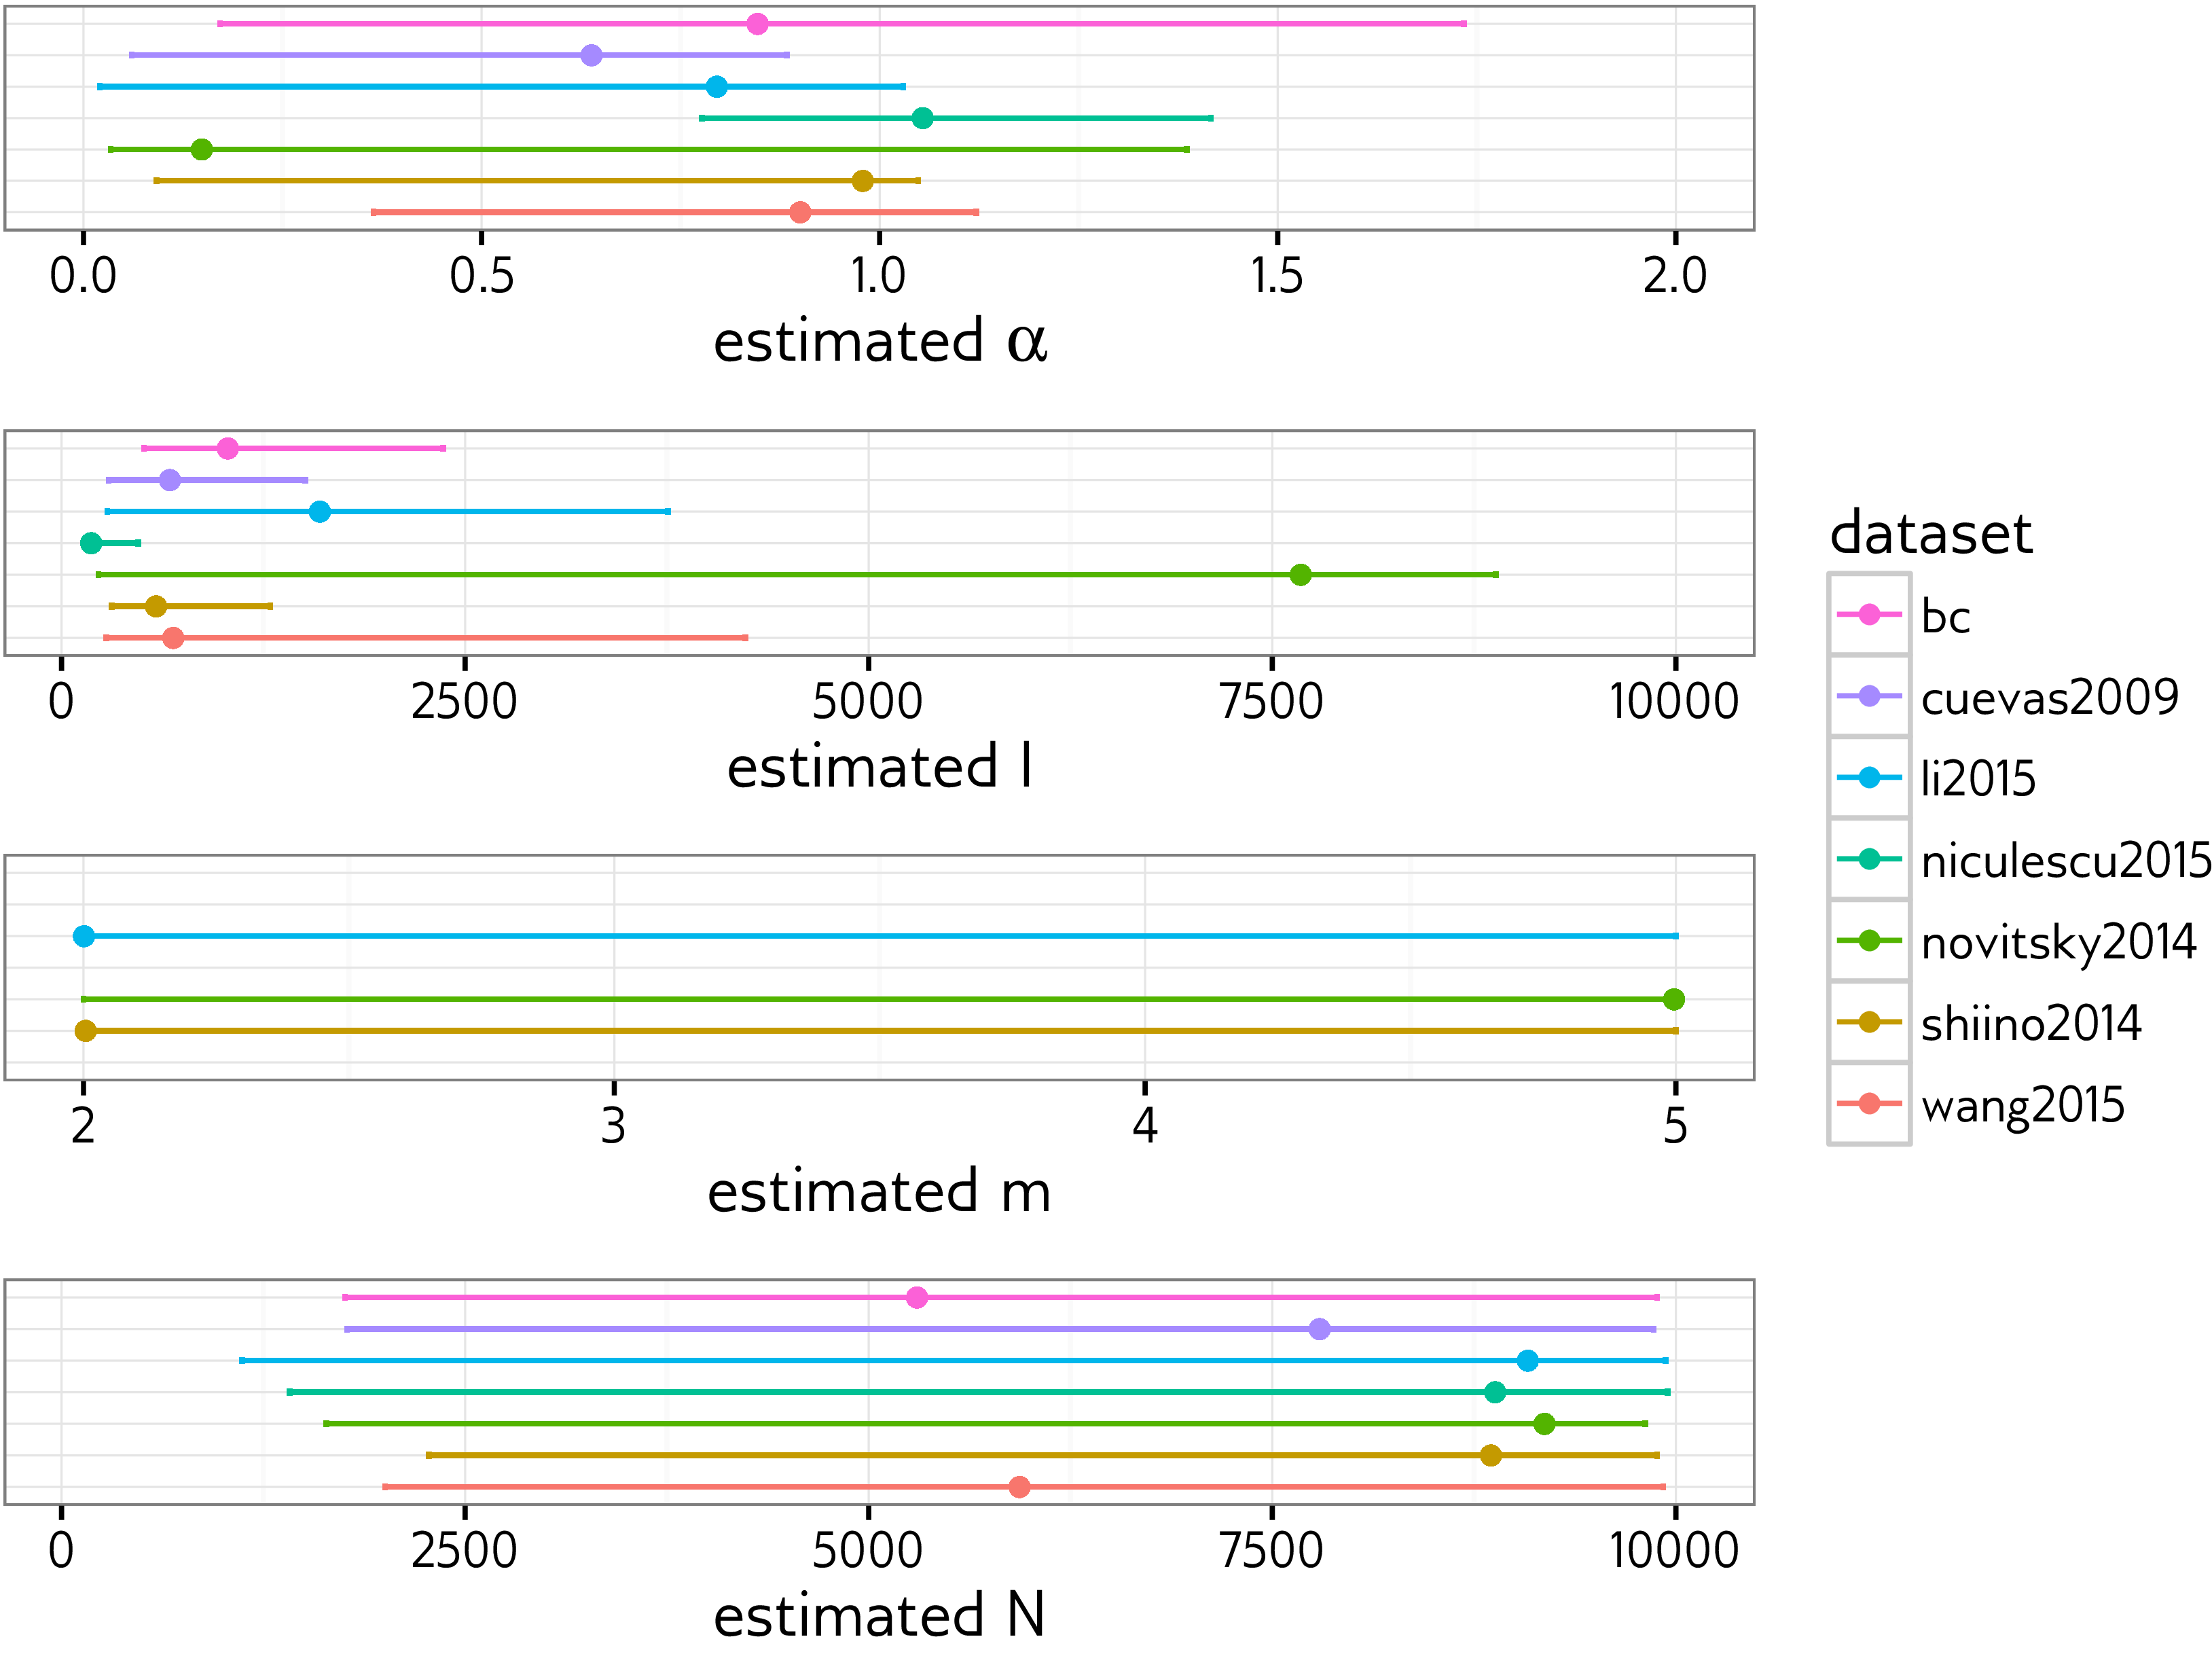
\includegraphics[trim=3.4in 1.5in 0 2.0in, clip, width=0.5\textwidth]{realdata-hpd-bc}
\end{frame}

\begin{frame}{Conclusions}
  \begin{itemize}
    \item We developed a phylodynamic method to fit contact network models to
      phylogenetic data.
      \pause
    \item The preferential attachment power of the Barab\'asi-Albert network
      model, which is challenging to estimate by traditional epidemiological
      methods, can be estimated with ABC.
      \pause
    \item The networks underlying real epidemics are heterogeneous,
      underscoring the importance of considering network structure in
      phylodynamic analyses.
  \end{itemize}
\end{frame}

\begin{frame}{Acknowledgements}
  \begin{columns}
    \begin{column}{0.6\textwidth}

      \textbf{BC Centre for Excellence in HIV/AIDS}

      Art Poon

      Jeff Joy

      Richard Liang

      Thuy Nguyen

      P. Richard Harrigan

      \hfill\\
      \textbf{University of British Columbia}

      Sarah Otto

      Alexandre Bouchard-C\^ot\'e

      \vfill
      \vspace{0.5cm}
      $\qquad\qquad$
\includegraphics[width=2cm]{logos/genomecanada}
      $\qquad$
      
\includegraphics[width=2cm]{logos/genomequebec}
    \end{column}
    \begin{column}{0.4\textwidth}
      \centering 

      
\includegraphics[width=3cm]{logos/cfe}
      \vspace{0.5cm}

      
\includegraphics[width=3cm]{logos/cihr}

      
\includegraphics[width=3cm]{logos/genomebc}

      
\includegraphics[width=3cm]{logos/bmgf}
      \vspace{0.5cm}

      
\includegraphics[width=3cm]{logos/btp}
    \end{column}
  \end{columns}
\end{frame}

\end{document}
